\RequirePackage{fix-cm}

\documentclass[12pt]{extarticle}

% \smartqed  % flush right qed marks, e.g. at end of proof

\usepackage{amsmath}
\usepackage{amsfonts}

% Specially for PMM: to have straight (upright) greek letters for vectors
%--------------------------------------
% \usepackage{upgreek}
% \usepackage[artemisia]{textgreek}
\usepackage[euler]{textgreek} %use upsilon instead of nu
%--------------------------------------

% Russian-specific packages
%--------------------------------------
\usepackage[T2A]{fontenc}
\usepackage[utf8]{inputenc}
\usepackage[russian]{babel}
%--------------------------------------

% Asymptote for pictures
%--------------------------------------
\usepackage{asymptote} %% comes with options inline and attach
%--------------------------------------

% graphicx for graphs
%--------------------------------------
\usepackage{graphicx}
%--------------------------------------

% so that it was possible to fix a figure's placement with [H]: \begin{figure}[H]
%--------------------------------------
\usepackage{float}
%--------------------------------------

% to put Fig.N on the margins
%-------------------------------------
\usepackage{marginnote}
\reversemarginpar
%-------------------------------------


%--------------------------------------
% Specially for PMM: make all imported EPS grayscale:
%--------------------------------------
\usepackage[gray]{epspdfconversion}
%--------------------------------------

% \usepackage{subfig} % incompatible with subcaption package
% \graphicspath{ % not used here
    % {./pic/,./asy/}
% }
%--------------------------------------

% subcaption for many figures under one big caption
% each having its own small caption
%--------------------------------------
%\usepackage{caption}
%\usepackage{subcaption}
%--------------------------------------

% so that refs were [1-10], not [1,2,3,4,5,...]
%--------------------------------------
\usepackage{cite}
%--------------------------------------

% to get \bigstar
%--------------------------------------
\usepackage{amssymb}
%--------------------------------------

% \ddfrac command to show big fractions, not cramped up
% https://tex.stackexchange.com/questions/173899/
%--------------------------------------
\newcommand\ddfrac[2]{\displaystyle\frac{\displaystyle #1}{\displaystyle #2}}
%--------------------------------------

% \vsp command to make a spacey newline
% useful for equations arrays
%--------------------------------------
\newcommand\vsp[1][10]{\\[#1pt]}
%--------------------------------------

% to customize itemize
%--------------------------------------
\usepackage{enumitem}
%--------------------------------------

% to set text width
%--------------------------------------
% \usepackage{geometry}
\usepackage{changepage}
%--------------------------------------



% partial derivatives (can \usepackage{physics}, but only one command so far, so no)
%--------------------------------------
\newcommand\pd[2]{\frac{\partial #1}{\partial #2}}
\newcommand\ddpd[2]{\ddfrac{\partial #1}{\partial #2}}
\newcommand\ddt[1]{\frac{d #1}{dt}}
\newcommand\ddddt[1]{\ddfrac{d #1}{dt}}
%--------------------------------------

% unbreakable space parenthesized reference
%--------------------------------------
\newcommand\upr[1]{~(\ref{#1})}
%--------------------------------------

% Nice letters
%--------------------------------------
\newcommand\M[0]{\mathcal{M}} % Matrix of intertia
\newcommand\const{\mathrm{const}} %константа
\newcommand\AntiU[0]{\mathcal{U}} % Helper antisymmetric matrix for eqs' RHS
\newcommand\Rhs[0]{\mathcal{R}} % RHS
\newcommand\Prhs[0]{\mathcal{P}} % The family of matrices for RHS
\newcommand\prhs[0]{\mathbf{p}} % Poisson brackets
\newcommand\vnu[0]{\text{\textbf{\textupsilon}}} % Upright greek vector nu for PMM
%--------------------------------------

% change line spacing mid doc (affects global line spacing)
%--------------------------------------
% \usepackage{setspace}
%--------------------------------------


\renewcommand{\vec}[1]{\boldsymbol{\mathbf{#1}}}
%\renewcommand{\figurename}{Фиг.}
\usepackage[labelsep=period]{caption}
\addto\captionsrussian{\renewcommand{\figurename}{Фиг. }}

\newtheorem{stmt}{Утверждение}
\newtheorem{prblm}{Затруднение}

% biblio hacks -- noindent bibitems
\makeatletter
\renewenvironment{thebibliography}[1]
      {\section*{\refname}%
      \@mkboth{\MakeUppercase\refname}{\MakeUppercase\refname}%
      \list{\@biblabel{\@arabic\c@enumiv}}%
            {\settowidth\labelwidth{\@biblabel{#1}}%
             \leftmargin\labelwidth
             \advance\leftmargin-25pt% change 20 pt according to your needs
             \advance\leftmargin\labelsep
             \setlength\itemindent{25pt}% change using the inverse of the length used before
             \@openbib@code
             \usecounter{enumiv}%
             \let\p@enumiv\@empty
             \renewcommand\theenumiv{\@arabic\c@enumiv}}%
      \sloppy
      \clubpenalty4000
      \@clubpenalty \clubpenalty
      \widowpenalty4000%
      \sfcode`\.\@m}
      {\def\@noitemerr
        {\@latex@warning{Empty `thebibliography' environment}}%
      \endlist}
\renewcommand\newblock{\hskip .11em\@plus.33em\@minus.07em}
\makeatother


\voffset=-15mm \textwidth=17cm \textheight=24cm
\oddsidemargin=0cm \topmargin=+0cm \headsep=10pt \evensidemargin=0mm
\renewcommand{\baselinestretch}{2}

\makeatletter \@addtoreset{equation}{section} \makeatother
\makeatletter

% bibliography hacks
\renewcommand{\@biblabel}[1]{#1. \hfill}
\makeatother
\addto\captionsrussian{\def\refname{Литература}}
\renewcommand{\refname}{}

\renewcommand{\thesection}{\arabic{section}}
\renewcommand{\theequation}{\arabic{section}.\arabic{equation}}


\begin{document}

% \chapter[Уравнения движения экипажа на~омни-колесах с~учетом динамики роликов]{Уравнения движения \\ экипажа~на~омни-колесах \\ с~учетом~динамики~роликов}


% % \filbreak
ОБЗОР ЛИТЕРАТУРЫ
% \begin{itemize}
%     \item Омни-колеса
%     \begin{itemize}
%         \item Определение омни-колеса
%         \item Работы по омни-экипажам в постановке без роликов
%         \item Работы Адамова в постановке с одним роликом
%         \item Работы о технических реализациях и front-to-back
%         \item Работы об управлении
%         \item Работы о шарах
%     \end{itemize}
%     \item Системы тел и удары
%     \begin{itemize}
%         \item Сложностей с количеством роликов и сменами контакта
%         \item Подходы к описанию динамики систем тел
%         \item Основания теории удара
%         \item Односторонние связи и удары в системах тел
%         \item Формализм языка Modelica
%         \item Работы по омни-колесам на Modelica
%     \end{itemize}
% \end{itemize}


Основной областью, в которой омни-колеса находят применение, является робототехника \cite{Seeni2010,Martynenko2005,GolubevSnake2004}. Экипажи с омни-колесами и колесами \textit{mecanum} \cite{Ilon} подробно описаны в обзорных работах в этой области \cite{Campion1996,Zimmermann2009,ChungIagnemma2016,Kanjanawanishkul2015,Adascalitei2011} как с точки зрения теоретической механики, так и с позиции технической реализации систем. Геометрия поверхности ролика отдельно рассмотрена в \cite{Gfrerrer2008}, где показано, что это алгебраическая поверхность восьмого порядка, построена аппроксимация поверхности ролика тором и сформулировано условие корректности конфигурации омниколесного экипажа: оси всех роликов, контактирующих с опорной плоскостью, не должны проходить через одну точку или быть параллельны, иначе экипаж не способен совершать ряд движений.

Движение экипажа с омни-колесами по абсолютно шероховатой плоскости рассмотрено в \cite{ZobovaTatarinovAspecty2006,zobova2008svobodnye8020851,ZobovaTatarinovPMM,Zobova2011}. Уравнения движения произвольной конфигурации экипажа получены, например, в \cite{ZobovaTatarinovPMM}, где также найдены их первые интегралы и инвариантная мера. Изучается конфигурация с тремя колесами, в которой два колеса имеют общую ось, а третье -- ось, перпендикулярную ей. Изучается устойчивость управляемых движений. Уравнения управляемого движения составлены методом Я.В.Татаринова (уравнения в лаконичной форме) \cite{Tatarinov,Tatarinov2005}. В \cite{Zobova2011} этот метод получения уравнений движения  проиллюстрирован на примере омниколесного экипажа, а также рояльного колеса и экипажа с дифференциальным приводом.

В работе \cite{formalskii} рассмотрена симметричная конфигурация экипажа с омни-колесами, в которой центры колес расположены в углах правильного треугольника, а их плоскости вертикальны и перпендикулярны радиусам-векторам центров колес, выпущенным из центра треугольника. Описана ее кинематика, и рассматриваются движения по инерции и при постоянных напряжениях, подаваемых на моторы постоянного тока, установленные в осях колес. Дана оценка мощности, потребляемой моторами, и показано, что она наименьшая при движении в направлении оси одного из колес. Строится алгоритм отслеживания направления движения экипажа. Развитием этой работы стало рассмотрение экипажа со смещенным центром масс \cite{Martynenko2010_rus}, где построены траектории свободного движения и изучены вопросы существования движений по прямой и по окружности.

Движение экипажа произвольной конфигурации по инерции по абсолютно шероховатой плоскости рассматривается и в \cite{Borisov2011}, где также строятся различные примеры движения по инерции, в том числе, периодического; получены уравнения движения омниколесного экипажа на сфере. Позже в \cite{KilinBobykin2014} изучена управляемость экипажа произвольной конфигурации на абсолютно шероховатой плоскости и осуществимость движения по любой наперед заданной траектории.

Кроме экипажей, двигающихся за счет взаимодействия колес и опорной поверхности, изучаются и другие конструкции, например, шарообразные роботы, управляемые изнутри симметричным омниколесным экипажем \cite{Karavaev2015},
% Подходы к управлению: квази-статический и с переходными этапами.
либо двумя омниколесами,  установленными на сфере меньшего радиуса, находящейся внутри внешней сферы \cite{Ivanov2015a}. Последняя статья содержит также более широкий обзор литературы о роботах-шарах. Кроме того, в ней найдены условия, при которых возможно движение робота-шара вдоль произвольной траектории. Работа выполнена в формализме алгебры кватернионов. Известны и конструкции шарообразных роботов, управляемых двумя обычными колесами \cite{Zhan2011}, однако роботы, рассмотренные в \cite{Ivanov2015a}, имеют преимущество в способности нести полезный груз. Омни-колеса можно применять не только для перемещения в пространстве, но и для изменения ориентации тел. К примеру, в \cite{Weiss2015,Plumpton2014} предлагается использовать сферу, приводимую в движение омни-колесами, касающимися ее извне, в качестве корпуса тренажера для пилотов. В работе \cite{Plumpton2014} рассматривается точечный контакт колес и сферы, в \cite{Weiss2015} их взаимодействие задается в контактной модели Герца.

Инерцией движения роликов в большинстве работ  пренебрегают. Однако в работе \cite{Adamov2018}, опубликованной летом 2018 года, рассматривающей движение экипажа с четырьмя колесами \textit{mecanum}, учтено движение контактного ролика с учетом вязкого трения в осях колес и роликов. Уравнения движения строятся методом Аппеля. При этом предполагается, что точка контакта всегда находится строго под центром колеса. Изучается структура управляющих моментов на примере движения экипажа по окружности, а также устойчивость движения в линейном приближении. Отдельной областью интересов является определение коэффициентов в уравнениях движения \cite{Adamov2018a} в случаях, когда технические характеристики систем оказываются неизвестны, либо изменяются в процессе движения.

Отметим отдельно многочисленные работы по омни-роботам, содержащие описания практических реализаций  экипажей. Такие экипажи часто используются на соревнованиях мобильных роботов. К примеру, в \cite{Indiveri2007} описывается кинематика и строится управление симметричным омниколесным экипажем в условиях ограниченности моментов, прилагаемых двигателями. В \cite{Wada2007} строится гибридный экипаж с двумя обычными колесами и двумя роликонесущими. Весьма распространены работы, описывающие  низкоуровневую техническую реализацию экипажей, такие как \cite{Mohamed2017,Krishnaraj2017,SalamAl-Ammri2010}. В практике мобильных роботов необходимой задачей является навигация. В \cite{Eng2010} рассматривается способ навигации омни-колесных экипажей с помощью так называемого многочастичного фильтра \cite{Gordon1993}, широко распространенного в робототехнике метода решения нелинейных задач оценивания \cite{DelMoral1997}. Для омни-колес важен характер поверхности, по которой экипаж движется. Поэтому в работе \cite{Vicente2015} строится метод определения типа материала опорной поверхности с помощью оценивания вибраций при движении с целью адаптации управления: движение по мягким поверхностям естественным образом оказывается медленнее, а движение по жестким вызывает б\textit{о}льшие вибрации, что требуется компенсировать управлением. Предлагается также модель, в которой колеса экипажа подпружинены для компенсации неровности поверхности \cite{NguenMAI2012}.

Следующие работы посвящены оптимальному управлению движением омни-экипажей
по кинематическим связям.
В работе \cite{Ashmore2002a} показано, что перемещение омни-экипажа между двумя точками на плоскости происходит быстрее всего не по прямой, а по дуге окружности. В \cite{Balkcom2006} оптимальные по времени траектории рассмотрены существенно детальнее, их построение проводится с помощью принципа максимума Понтрягина, и строится классификация таких траекторий. Класс работ о построении управляемых движений весьма широк \cite{Huang2015,Bramanta2017,Kalmar-Nagy2016,Szayer2017}, имеются работы с управлением с учетом динамики системы. Встречаются работы, рассматривающие ситуацию частичного отказа приводов \cite{Field2017,Ivanov2015a}.

Интересны работы, описывающие все стадии разработки робототехнической платформы с омни-колесами, от кинематики и уравнений движения до построения (оптимального) управления, включающие также технические реализации экипажей \cite{Williams2002,Purwin2006,Li2009}. В \cite{Galicki2009} построено управление с объездом препятствий. В \cite{Lin2013} рассматривается адаптивное управление с учетом переменных коэффициентов трения в точках контакта, а также массы платформы.

Перейдем теперь к обзору формализмов, используемых при построении динамических уравнений систем твердых тел. 

Для описания систем многих тел, в том числе, систем, организованных иерархически, известны различные подходы \cite{Wittenburg2008,EberhardSchiehlen,Jain2011,Roberson1988,Jerkovsky1977}. Классические подходы основаны на теории графов \cite{Wittenburg2008,Jerkovsky1977}. Разработаны рекурсивные методы для описания древовидных структур \cite{EberhardSchiehlen}. Весьма обширный обзор существующих методов для описания систем тел, в том числе, с замкнутыми кинематическими цепями, проведен в \cite{Jain2011}. Работа \cite{Roberson1988}, кроме непосредственно методов описания систем тел, уделяет отдельное внимание историческому контексту развития данной области, в частности, констатируя слабопреодолимые затруднения, возникающие в аналитическом исследовании из-за нелинейностей и количества тел в системах, а также подробно освещая их разрешение с помощью вычислительной техники, как основной метод их изучения и проектирования.

В отношении контактного взаимодействия твердых тел, при описании динамики омни-колес и экипажей можно либо идти по пути наложения дифференциальных связей отсутствия проскальзывания, либо вводить силу трения в контакте. Динамика систем с дифференциальными связями подробно описана, например, в \cite{Chaplygin1949,NejmarkFufaev1967}. В \cite{NejmarkFufaev1967} и \cite{karapetyan1981negolonom}, в частности, подробно обсуждается вопрос обоснованности подобных идеализаций. В главах 1 и 2 настоящей работы принимается модель точечного контакта ролика и опорной плоскости. Для получения уравнений движения таких систем часто пользуются методами Аппеля либо Лагранжа первого рода \cite{KarapetyanKugushev2010,Appel1,AppelTwo1960}. В силу объема требуемых выкладок в рассматриваемой системе мы применили метод получения уравнений движения в лаконичной форме Я.В. Татаринова \cite{Tatarinov,Tatarinov2005}.

В отсутствии проскальзывания отдельного рассмотрения требует смена ролика в контакте с опорной плоскостью. Явления, возникающие при подобных движениях, описываются теорией удара \cite{AppelTwo1960,Vilke,KozlovTreshevBilliardsBook1991}. В \cite{KozlovTreshevBilliardsBook1991} приведено формальное построение этой теории, и обсуждается ее физическая обоснованность. Всестороннее современное рассмотрение механики систем с односторонними связями с учетом их моделирования с помощью вычислительной техники содержится в \cite{BrogliatoBook1999}, а также в серии работ \cite{PfeifferGlockerBook,PfeifferGlocker1995,Pfeiffer1999a,PfeifferGlockerSymposium1999,Pfeiffer1997,Glocker1999,Pfeiffer2001,Brogliato2002,Pfeiffer2003,FloresGlocker2011,Zbiciak2014}. Уравнения движения для систем с односторонними связями в интегральной форме построены в \cite{Kugushev2003}, и там же рассмотрены удары, в частности, о дифференциальные связи.

Постановка задачи с сухим трением в контакте между роликом и опорной плоскстью приводит к дальнейшему усложнению задачи. Методы исследования истем с сухим трением описаны в \cite{PfeifferGlocker1993,Pfeiffer1996,Anitescu1997,Lacoursiere2011,Charles2014,Paoli2015,Moreau1988}, а также \cite{Novozhilov1991} Исследование омниколесного экипажа с учетом динамики всех роликов и трения возможно лишь численно, и здесь, кроме понимания природы трения, требуется подходящий формализм для создания компьютерной модели экипажа. Нами был выбран формализм языка Modelica \cite{ModelicaSpec,Dymola,Fritzson}, примененный ранее к задачам динамики систем тел \cite{KosenkoQuaternionRus,Kosenko2006unilat,Kosenko2006,Kosenko2007,KosenkoGraphs2009,KosenkoGusev2012,KosenkoRolling,Kosenko2006,KosenkoAlexandrov,KosenkoKuznetzova}. Этот метод уже использовался и при изучении динамики омниэкипажей \cite{Kalman2012assistant,Kalman2013control,Kalman2013braking,Kalman2013practical}. В этих работах рассматривается контакт с трением, но ролики имеют существенно упрощенную форму -- считаются массивными цилиндрами либо конусами. Автор утверждает, что полученная им модель слишком медленна и сложна, и потому строит еще одну упрощенную модель, полностью пренебрегая инерцией роликов, но учитывая  трение в направлении оси ролика. В \cite{Kalman2013braking} изучается вопрос заноса омни-колесных экипажей при торможении в упрощенной модели.

Первая глава представленной работы, где получены уравнения движения экипажа с массивными роликами без проскальзывания, принята к печати \cite{GerasimovZobovaPMM2018}. Вторая глава, содержащая модель перехода с одного ролика на другой с позиции теории удара, принята к печати \cite{GerasimovZobovaTrudyMAI2018}. В работах \cite{KosenkoGerasimovNd2016,KosenkoGerasimovJsme2016} опубликованы результаты третьей главы, в которой экипаж моделируется в постановке с регуляризованным сухим трением в точечном контакте ролика и опорной плоскости. Эти результаты доложены  конференциях и опубликованы в их сборниках трудов \cite{Kosenko2014unilateral,KosenkoGerasimov2014,Kosenko201construction,Kosenko2015verification,Kosenko2015hierarchy,KosenkoGerasimov2015,Kosenko2016testbench}.\\

% Ранее была рассмотрена динамика омни-экипажей с использованием упрощенных моделей омни-колес без учета инерции и формы роликов \cite{ZobovaTatarinovPMM, formalskii, borisov, ZobovaTatarinovAspecty2006, zobova2008svobodnye8020851, Martynenko2010_rus}, колеса (без роликов) моделируются как жесткие диски, которые могут скользить в одном направлении и катиться без проскальзывания в другом. Далее будем называть такую модель безынерционной, в том смысле, что инерция собственного вращения роликов в ней не учитывается. В другой части работ по динамике омни-экипажа \cite{KosenkoGerasimov, Tobolar, Williams2002, Ashmore2002} используются некоторые формализмы для построения численных моделей систем тел. При этом явный вид уравнений движения оказывается скрытым, что делает невозможным непосредственный  анализ уравнений и затрудняет оценку влияния разных факторов на динамику системы.


% СОДЕРЖАНИЕ РАБОТЫ

Настоящая работа состоит из введения, трех глав, заключения и списка литературы.

Во введении дано описание предметной области и цели данной работы, выполнен обзор литературы об омни-колесах и экипажах, оснащенных ими, о динамике систем тел, в том числе, с односторонними связями, ударами и трением, а также составлено краткое содержание работы.

Целью работы является изучение неуправляемого движения роликонесущего экипажа по горизонтальной плоскости с учетом инерции роликов и трения в двух постановках. В первой постановке опорная плоскость абсолютно шероховата, т.е. проскальзывание между роликом в контакте и плоскостью отсутствует. При этом предполагается, что при смене ролика в контакте происходит мгновенное согласование скоростей системы в соответствии с новыми связями (удар связями). Во второй между контактным роликом и опорной плоскостью действует сила сухого трения скольжения Кулона, либо сила вязкого трения скольжения. 

Экипаж состоит из несущей платформы и трех одинаковых омни-колес, центры которых расположены в вершинах правильного треугольника, а плоскости препендикулярны биссектрисам соответствующих углов. Омни-колесо моделируется абсолютно твердым диском и некоторым количеством распределенных по его окружности весомых роликов, свободно вращающихся вокруг своих осей, направленных вдоль касательных к окружности.

В первой и второй главе работы рассматривается движение  экипажа по абсолютно  шероховатой плоскости, т.е. предполагается, что проскальзывание между опорным роликом и плоскостью отсутствует. Уравнения движения получены в явном виде с использованием формализма лаконичных уравнений Я.В. Татаринова. Изучена структура уравнений, найдены первые интегралы и проведено сравнение с уравнениями движения безынерционной модели. Показано, что если момент инерции ролика относительно его оси равен нулю, то уравнения совпадают с уравнениями безынерционной модели.

Во второй главе рассмотрена задача о смене ролика в контакте: при повороте колеса вокруг своей оси в контакт с плоскостью приходит новый ролик, скорость которого, вообще говоря, не согласована со связями, при этом возникает проскальзывание. Предполагается, что проскальзывание прекращается за бесконечно малый промежуток времени. Составлены линейные алгебраические уравнения, определяющие обобщенные скорости после смены ролика в контакте в соответствии с теорией удара. Таким образом, численное моделирование движения экипажа состоит из решения задачи Коши уравнений, полученных в первой главе, пока в контакте находится один и тот же ролик, и решения линейных алгебраических уравнений при смене ролика для получения начальных условий для следующего гладкого участка. Получены и проанализированы численные решения для симметричной конфигурации экипажа.

В третьей главе построена динамическая модель экипажа на плоскости с сухим трением Кулона-Амонтона, регуляризованным в окрестности нуля по скоростям участком линейной функции насыщения с достаточно большим угловым коэффициентом. Особое внимание уделяется вопросу моделирования неудерживающей связи в контакте ролика и горизонтальной плоскости, отслеживанию точки контакта ролика и опорной плоскости, а также алгоритмической реализации процесса переключения контакта от ролика к ролику при качении омни-колеса. Динамическая модель построена в формализме объектно-ориентированного моделирования на языке Modelica. Выполнена верификация динамической модели с использованием безынерционной модели.

В заключении перечислены результаты работы.

По результатам работы опубликованы и приняты к печати в рецензируемых журналах, реферируемых в международных базах WebOfScience, Scopus, RSCI и входящих в список ВАК, следующие статьи \cite{KosenkoGerasimovNd2016,GerasimovZobovaPMM2018,GerasimovZobovaTrudyMAI2018,KosenkoGerasimovJsme2016,KosenkoGerasimov2015,Kosenko201construction}

Результаты докладывались автором на ряде международных и всероссийских конференциях: Международная конференция по дифференциальным уравнениям и динамическим системам 2018, Суздаль, Россия, 6-11 июля 2018; 20-е Международное рабочее совещание по компьютерной алгебре (Дубна, 21-22 мая 2018), Дубна, Россия, 21-22 мая 2018; Ломоносовские Чтения - 2018, МГУ имени М.В. Ломоносова, Россия, 16-25 апреля 2018; Ломоносовские чтения - 2017, МГУ имени М.В. Ломоносова, Россия, 17-26 апреля 2017; 11th International Modelica Conference Versailles, France, September 21-23, 2015. Результаты также были представлены аспирантом на семинаре Аналитическая механика и теория устойчивости (имени В.В. Румянцева) под руководством д.ф.-м.н. проф. А.В. Карапетяна в 2017 и 2018 г. и на семинаре Динамика относительного движения под руководством д.ф.-м.н. проф. В.Е. Павловского на механико-математическом факультете МГУ им. М.В. Ломоносова в 2018 г.

% \chapter[Уравнения движения экипажа на~омни-колесах с~учетом динамики роликов]{Уравнения движения \\ экипажа~на~омни-колесах \\ с~учетом~динамики~роликов}


% \section{Наложение связи при смене ролика в контакте}

\begin{figure}[h]
    \minipage{0.5\textwidth}
        \centering
        \asyinclude{./asy/pic_react}
        \caption{Реакции}
        \label{fig:react}
    \endminipage
    \minipage{0.5\textwidth}
        \centering
        \asyinclude{./asy/pic_project}
        \caption{Проекция}
        \label{fig:project}
    \endminipage
\end{figure}

В реальной системе при смене контакта имеет место скольжение роликов относительно плоскости, и при этом полная энергия системы рассеивается. В данной работе будем считать, что трение достаточно велико, и прекращение проскальзывания вновь вошедшего в контакт ролика происходит мгновенно. Это взаимодействие будет рассматриваться как абсолютно неупругий удар, происходящий при мгновенном наложении связи.
Освободившийся ролик начинает свободно вращаться вокруг своей оси.
Будем предполагать следующее:
\begin{itemize}
    \item удар происходит за бесконечно малый интервал времени $\Delta t << 1$, так что изменения обобщенных координат пренебрежимо малы $\Delta \q \sim \dotq\Delta t << 1$, а изменения обобщенных скоростей конечны $\Delta \dotq < \infty$;
    \item взаимодействие экипажа с опорной полоскостью во время удара сводится к действию в точках контакта нормальных и касательных реакций $\mathbf{R}_i = \mathbf{N}_i + \mathbf{F}_i$ с нулевым моментом $\mathbf{M}_i = 0$;
    \item к моменту окончания удара $t^*+\Delta t$ уравнения связей выполнены $\dqposle = \cstr(\q)\nuposle$, т.е. за время $\Delta t$ проскальзывание вошедшего в контакт ролика заканчивается.
\end{itemize}

% Таким образом, решение задачи представляется в виде чередования гладких участков, определяемых уравнениями движения, и пересчетов значений обобщенных скоростей в моменты смен контакта.

Исходя из этих предположений, в следующих разделах получим системы алгебраических уравнений, связывающих значения обобщенных скоростей непосредственно перед ударом $\dqdo$ и значения псевдоскоростей сразу после удара $\nuposle$ двумя разными способами: в первом случае, будем  вводить ударные реакции, действующие в точках контакта, а во втором, будем рассматривать неупругий удар как проецирование вектора обобщенных скоростей на плоскость, задаваемую уравнениями вновь налагаемых связей.

Таким образом, моделирование системы состоит в решении задачи Коши системы обыкновенных дифференциальных уравнений в интервалах между моментами смены роликов в контактах и решения систем алгебраических уравнений в эти моменты для получения начальных условий для следующего безударного интервала.

% \subsection{Способ 1. Классическая механика}
Составим алгебраические уравнения, связывающие значения псевдоскоростей после удара и величины ударных импульсов. В течение бесконечно малого времени $\Delta t$ наложены только геометрические связи, так что скорости $\dot{\mathbf{q}}$ независимы. Запишем уравнение удара в обобщенных координатах \cite{Vilke}:
\begin{equation}\label{eq:udar_general}
\eqDeltaqQ,
\end{equation}
где $\mke$ -- матрица кинетической энергии без учета связей (так что $\M^* = \cstr^T \mke \cstr$), а $\Q$ -- вектор ударных импульсов обобщенных сил $\Q$:
\begin{equation*}
\eqQ
\end{equation*}
Исходя из геометрии системы (см. фиг.~\ref{fig:react}), получаем, что компоненты этого вектора связаны с касательными составляющими реакций следующим образом:
\begin{eqnarray*}
\eqQiOne \\
\eqQiTwo \\
\eqQiTheta \\
\eqQChii \\
\eqQPhii \\
\eqQs
\end{eqnarray*}
В матричном виде:

\begin{equation*}
\eqQKFmat
\end{equation*}
Размерность матрицы $\mK$ равна $(3 + N(n+1)) \times 2N$, и её ранг максимален.

Непосредственно перед ударом связи, запрещающие проскальзывание в точках касания роликов, находящихся в контакте в этот момент, снимаются.
В момент сразу после удара аналогичные связи налагаются на вновь входящие в контакт ролики.
\begin{equation*}
\eqqnu
\end{equation*}

Тогда уравнение\upr{eq:udar_general} можно записать в виде:
\begin{equation*}
\eqMVnuKF
\end{equation*}
Полученная линейная система относительно $\nuposle$ и $\F$ допускает единственное решение.

% Либо в матричной форме
% \begin{equation*}
% \eqMVnuKFmat
% \end{equation*}

% Решение тогда получается следующим образом
% \begin{equation*}
% \eqMVnuKFmatres
% \end{equation*}
% где матрица $\mvk$ обратима в силу геометрии системы.
% %
\subsection{Способ 2. Аналитическая механика}

Мотивация -- строго определяется матрицами кинетической энергии и связей, не требует произвольного введения векторов реакций.

\begin{itemize}
    \item постановка задачи теории удара как проецирования вектора обобщенных скоростей на плоскость в пространстве виртуальных перемещений, определяемую вновь налагаемыми связями
    \item выражение для скоростей после удара
\end{itemize}

Связи, налагаемые в момент смены контакта, задают подпространство $\subspace$ в пространстве виртуальных перемещений.

Вектор обобщенных скоростей до удара $\dqdo$ может иметь составляющую $\deltadq$, ортогональную этому подпространству (в кинетической метрике). (А ПОЧЕМУ ИМЕННО В КИНЕТИЧЕСКОЙ?! КАК-ТО КРАСИВО НАДО СКАЗАТЬ)

В силу идеальности налагаемых связей, значения обобщенных скоростей после удара можно получить вычитанием этой компоненты из $\dqdo$ или, что то же, проецированием $\dqdo$ на подпространство $\subspace$.

Найдем вектор $\deltadq$, ортогональный $\subspace$ в метрике, задаваемой матрицей кинетической энергии $\mke$, такой что $\dqposle = \dqdo - \deltadq = \mathbf{V}\nuposle \in \subspace$

\begin{equation*}
\eqDelta
\end{equation*}
\begin{equation*}
\logicDeltaOrth
\end{equation*}

откуда
\begin{equation*}
\eqnuposleproj
\end{equation*}
где матрица $\cstr^T\mke\cstr$ обратима, поскольку имеет максимальный ранг.
% 
\subsection{Разрешимость основного уравнения теории удара при наложении дифференциальных связей}

Покажем существование и единственность решения уравнения\upr{eq:udar_mat} для более общего случая.
Рассмотрим натуральную систему с обобщенными координатами $\q$ и кинетической энергией $T = \ddfrac{1}{2}(\mke\dotq, \dotq)$, на которую в момент времени $t^*$ мгновенно налагаются дифференциальные связи вида $\A\dotq = 0$.
При этом верно основное уравнение удара\upr{eq:udar_general}.
Будем считать также, что выполнено условие идеальности связей:
\begin{equation}\label{eq:constraints_ideal}
    \Q^T \delta\qposle = 0,
\end{equation}
где $\delta\qposle$ -- виртуальные перемещения системы после наложения связей.

Обобщенные скорости системы после наложения связей $\dqposle$ лежат в линейном подпространстве $\subspace = \ker \A$ пространства виртуальных перемещений $T_\q\M$.
В этом подпространстве можно выбрать базис, и таким образом ввести псевдоскорости на интервале после наложения связей: $\dqposle = \cstr\nuposle$, где столбцы матрицы $\cstr$ есть векторы базиса в $\subspace$.
При этом для матрицы оператора $\A$ и матрицы $\cstr$ будет выполнено:
\begin{equation}\label{eq:constraints_orth}
    \A\cstr = 0.
\end{equation}
Условие идеальности связей\upr{eq:constraints_ideal} означает, в частности, что вектор импульса ударных реакций $\Q$ лежит в подпространстве $T_\q\M$, дополнительном к $\subspace = \ker \A$, и таким образом, по лемме о множителях Лагранжа \cite{KarapetyanKugushev2010} представляется в базисе, составленном из строк матрицы $\A$: $\Q = \A^T\lagr$, где $\lagr$ -- множители Лагранжа.

Уравнение удара\upr{eq:udar_general} тогда можно представить в виде:
\begin{equation}\label{eq:udar_mat_At}
    \mke\cstr\nuposle - \A^T\lagr = \mke\dqdo.
\end{equation}
% где вместо матрицы $\mK$, приведенной в разделе~\ref{sect:impact_classical}, стоит любая матрица оператора связей~$\A$.

Равенство\upr{eq:udar_mat_At} есть система алгебраических уравнений относительно вектора неизвестных $(\nuposle, \lagr)^T$. Матрица $(\mke\cstr; -\A^T)$ этой системы -- невырожденная квадратная размера~$\dim~\q~\times~\dim~\q$, поскольку столбцы $\cstr$ и $\A^T$ образуют базисы в дополнительных подпространствах $T_\q\M = \mathbb{R}^{\dim \q}$. Доказательство невырожденности этой матрицы носит технический характер и проведено в Приложении. Таким образом, задача теории удара в рассматриваемом случае всегда имеет решение, решение единственно и доставляет одновременно значения обобщенных скоростей после удара $\dqposle = \cstr\nuposle$ и импульсов ударных реакций~$\Q = \A^T\lagr$.

Отметим также, в силу основного уравнения удара\upr{eq:udar_general} и условия идеальности\upr{eq:constraints_ideal}, мгновенное наложение связей можно рассматривать как абсолютно неупругий удар при котором теряется компонента $\deltadq$ вектора обобщенных скоростей $\dqdo$, ортогональная подпространству $\subspace$ в кинетической метрике:
\begin{equation*}
    \deltadq^T\mke\delta\q = 0.
\end{equation*}
Тогда вектор обобщенных скоростей после удара $\subspace \ni \dqposle = \dqdo - \deltadq$ вычисляется непосредственно как проекция вектора $\dqdo$ на подпространство $\subspace$, минуя получение импульсов ударных реакций $\Q$. Явный вид матрицы $\A$ также не требуется, достаточно ввести псевдоскорости: $\dqposle = \cstr\nuposle$.
Выражение для $\nuposle$ тогда может быть получено следующим образом:
\begin{equation*}
    0 = \cstr^T\Q = \cstr^T\mke\deltadq = \cstr^T\mke(\cstr\nuposle - \dqdo) = \cstr^T\mke\cstr\nuposle - \cstr^T\mke\dqdo,
\end{equation*}
откуда:
\begin{equation*}
\eqnuposleproj.
\end{equation*}

Эту же формулу можно получить и из уравнения\upr{eq:udar_mat_At}, домножая его слева на $\cstr^T$ и пользуясь равенством\upr{eq:constraints_orth}. Симметрично, при умножении\upr{eq:udar_mat_At} слева на $\A\mke^{-1}$, имеем выражение для множителей Лагранжа $\lagr$:
\begin{equation*}
    \lagr = -(\A \mke \A^T)^{-1}\A\dqdo,
\end{equation*}
не включающее явно матрицу связей $\cstr$.

Вернемся к рассмотрению экипажа с омни-колесами. Покажем, как связаны матрица $\mK$ и вектор импульсов ударных реакций $\F$ в координатах $OXY$ с изложенными общими утверждениями.
Рассмотрим вектор $\mathbf{r} = ( x_1, y_1, z_1 \ldots, x_N, y_N, z_N )^T$, составленный из координат точек колес, находящихся в контакте с опорной плоскостью $C_i$ в неподвижной системе отсчета $OXYZ$.
Матрица $\A$ связей\upr{eq:constraints_vec} может быть получена, например, как матрица Якоби зависимости вектора $\mathbf{r}$ от обобщенных координат $\q$: $\A(\q) = \ddfrac{\partial \mathbf{r}(\q)}{\partial \q}\bigg|_{x,y}$.
Непосредственный подсчет показывает, что столбцы матрицы Якоби, соответствующие оси $OZ$, нулевые, и потому их следует исключить.
При этом матрица $\A^T$ в точности совпадает с матрицей $\mK$ из~раздела~\ref{sect:impact_classical}, и таким образом, вектор множителей Лагранжа $\lagr$ совпадает с вектором реакций $\F$.

% 
\subsection{Изменение кинетической энергии}
Выясним, как меняется кинетическая энергия при смене ролика в контакте:
$$
2\Delta\ke  =  2\left(\ke^+ - \ke^-\right) = \dotp{\mke\dqposle}{\dqposle} - \dotp{\mke\dqdo}{\dqdo} =
$$
$$
= \dotp{\mke\deltadq}{\deltadq} + 2\dotp{\mke\dqdo}{\deltadq} = -\dotp{\mke\deltadq}{\deltadq} + 2\dotp{\mke\dqposle}{\deltadq}
$$
Последнее слагаемое равно нулю в силу идеальности связей\upr{eq:constraints_ideal} и основного уравнения удара\upr{eq:udar_general}, т.е. равенства нулю мощности ударных импульсов на перемещениях, допускаемых связями
$$\logicWorkZero.$$
% (заметим: $\edMkeSim$) или, что то же, ортогональности в кинетической метрике вектора потерянных скоростей $\deltadq$ подпространству $\subspace$ пространства возможных перемещений, определяемому связями.
Таким образом, изменение кинетической энергии системы равно энергии потерянных скоростей $\deltadq = \dqposle - \dqdo$:
\begin{equation*}
\eqDeltaT,
\end{equation*}
что соответствует теореме Карно ССЫЛКА.

% 
\section{Численные эксперименты}

Проведены численные эксперименты, моделирующие движение экипажа по инерции для трех вариантов начальных условий (см. рис.~\ref{fig:nu_impact}).
\begin{enumerate}[wide]
    \item \label{sol:self_rot} Платформа экипажа имеет ненулевую угловую скорость относительно вертикальной оси, проходящей через центр масс экипажа; центр масс платформы покоится ($\nu_1(0) = \nu_2(0) = 0, \nu_3(0) = 1$) (рис.~\ref{fig:nu_impact_1},~\ref{fig:self_rot}).
    \item \label{sol:straight} Центр масс платформы имеет ненулевую скорость в направлении от центра экипажа к центру первого колеса, угловая скорость платформы равна нулю ($\nu_1(0) = 1, \nu_2(0) = \nu_3(0) = 0$) (рис.~\ref{fig:nu_impact_2},~\ref{fig:straight}).
    \item \label{sol:wrench} Платформа экипажа имеет ненулевую угловую скорость относительно вертикальной оси, проходящей через центр масс экипажа, и центр масс платформы имеет ненулевую скорость в направлении от центра экипажа к центру первого колеса ($\nu_1(0) = 1, \nu_2(0) = 0, \nu_3(0) = 1$) (рис.~\ref{fig:nu_impact_3},~\ref{fig:wrench}).
\end{enumerate}
Свободные ролики в начальный момент покоятся относительно дисков колес, $\nu_s(0) = 0$. Угловые скорости $\dot{\chi}_i$ собственного вращения дисков колес относительно платформы экипажа и угловые скорости $\dot{\phi}_{i\cdot}$ собственного вращения роликов, находящихся в контакте с опорной плоскостью в начальный момент времени задаются согласованными со связями~(\ref{constraint_roller_contact}),~(\ref{constraint_wheel_contact}). Такие же варианты начальных условий рассмотрены в \cite{GerasimovZobovaPMM2018}, где используется упрощенная модель изменения обобщенных скоростей при смене контакта.


\begin{figure}
    \centering
    \begin{subfigure}[t]{0.3\textwidth}
        \centering
        \asyinclude{content/pic/asy/pic_nu_self_rot.asy}
        \caption{Движение $1$}
        \label{fig:nu_impact_1}
    \end{subfigure}
    \quad
    \begin{subfigure}[t]{0.3\textwidth}
        \centering
        \asyinclude{content/pic/asy/pic_nu_straight.asy}
        \caption{Движение $2$}
        \label{fig:nu_impact_2}
    \end{subfigure}
    \quad
    \begin{subfigure}[t]{0.3\textwidth}
        \centering
        \asyinclude{content/pic/asy/pic_nu_wrench.asy}
        \caption{Движение $3$}
        \label{fig:nu_impact_3}
    \end{subfigure}
    \caption{Рассмотренные варианты начальных условий}
    \label{fig:nu_impact}
\end{figure}
    
Расчеты выполнены для симметричного трехколесного экипажа ($\alpha_i = \frac{2\pi}{N}(i - 1), N = 3$) с $n = 5$ роликами на колесе. Все величины, участвующие в уравнениях, безразмерны. В безразмерных единицах радиусы платформы и колеса $R = 0.15$ и $r = 0.05$, массы платформы, колеса и ролика $1$, $0.15$ и $0.05$, и момент инерции $B$ ролика относительно его оси вращения положен равным $B \approx 1.6 \cdot 10^{-5}$. Таково значение осевого момента инерции однородного цилиндра радиуса $\ddfrac{l-r}{2}$, где $r = l\cos\ddfrac{\pi}{n}$, и массы, равной массе ролика.
% Для безынерционной модели массо-инерционные характеристики колес положим соответствующими экипажу с пятью заблокированными роликами.

% Заметим, что снятие и наложение связей в момент контакта, вообще говоря, означает изменение системы уравнений движения. Однако в силу симметрии колеса, система после смены отличается от системы до смены лишь нумерацией роликов и углами поворота колес $\chi_i$.
% (ВАРИАНТ) % Стыковку гладких участков выполним, исходя из соображений, которые поясним на следующем примере. Рассмотрим два момента смены контакта на одном из колес: переход с ролика $1$ на ролик $2$ и переход с ролика $n - 1$ на ролик $1$. В силу симметрии колеса, система, перешедшая на второй ролик с первого, эквивалентна системе, перешедшей с ролика $n - 1$ на первый, с точностью до нумерации роликов и значений угла поворота колеса.
% Чтобы не менять вид уравнений движения -- а точнее, вид матрицы связей $\cstr$ -- выполним переобозначение в момент смены контакта и получим решение на следующем гладком участке, как решение той же системы уравнений, но с новыми начальными условиями. При смене ($\chi_i = \chi_i^+$) заменим $\chi_i = \chi_i^+$ на $\chi_i = \chi_i^-$ и циклически перенумеруем ролики. Если колесо поворачивается против часовой стрелки $\dot{\chi_i} > 0$ (см. рис.~\ref{fig:wheel}), сдвинем индексы вперед: $j \rightarrow j+1\mod n$. Также восстановим значения обобщенных скоростей до удара $\dqdo = \cstr\nudo$, и переобозначим углы поворота роликов $\phi_{ij}$ и псевдоскорости свободных роликов после удара $\nu^+_{s(i, j)}$ соответственно выполненной перенумерации роликов. При вращении колеса в другую сторону, выполним симметричные преобразования.

Во всех трех случаях наблюдается убывание кинетической энергии скачками в моменты смены контакта. В промежутки времени между сменами энергия остается постоянной, что свидетельствует о точности вычислений.

В вариантах \ref{sol:self_rot} и \ref{sol:straight} заметны переходные режимы вращения роликов в начале движения, когда колесо совершает первый оборот, и каждый ролик проходит полный круг, выходя из контакта и возвращаясь в него снова.

Расчеты показали, что в случае \ref{sol:self_rot} центр масс экипажа покоится, платформа экипажа вращается вокруг вертикальной оси, проходящей через ее центр. При этом угловая скорость платформы $\nu_3$ в среднем медленно убывает (немонотонно), уменьшается на 5\%  за безразмерное время $10^3$ от начала движения. На графике на рис.~\ref{fig:self_rot_nu3} представлен интервал $t < 25$. Кинетическая энергия системы также медленно убывает, см. рис.~\ref{fig:self_rot_T}. На более длительном интервале $0 < t < 1000$ заметно, что характер убывания угловой скорости платформы экипажа $\nu_3$ близок к линейному, см. рис.~\ref{fig:self_rot_T_long}. Кинетическая энергия $T$ убывает нелинейно, но при полученных значениях псевдоскорости $\nu_3$  нелинейность почти не различима в масштабе рисунка. На рис.~\ref{fig:self_rot_dphi} приведены скорости собственного вращения роликов на первом колесе $\dot{\phi}_{1j}$. Находящийся в контакте ролик неподвижен относительно колеса (в силу связи со скоростью центра масс, см.~(\ref{constraint_roller_contact})) при $\nu_1 = \nu_2 = 0$, чему соответствуют участки графиков, лежащие на оси абсцисс. Когда контакт этого ролика с опорной плоскостью прекращается, он начинает вращаться за счёт вращения экипажа в целом вокруг вертикальной оси (см. первый интеграл (\ref{int_free_roller}), существующий на гладких участках). После полного оборота колеса ролик приобретает некоторую скорость вращения, которую мгновенно теряет при следующем входе в контакт. В результате вся система теряет часть энергии, испытывая удар связями, запрещающими проскальзывание. Скорость $\nu_3$ вращения экипажа вокруг вертикальной оси при этом изменяется скачком (см. например $t=1, 3, 5, 7.5$ на графиках).

При движении \ref{sol:straight} угловая скорость $\nu_3$ тождественно равна нулю, центр масс совершает прямолинейное движение в направлении оси $OX$ неподвижной системы отсчета. Зависимости скорости центра масс экипажа $v = \sqrt{\nu_1^2+\nu_2^2}$ и кинетической энергии $T$ от времени показаны на рис.~\ref{fig:straight_Tv_long} и~\ref{fig:straight_Tv}. Обе величины убывают (энергия -- монотонно, скачками, с каждой сменой контакта; скорость центра масс -- в среднем). Переднее колесо не вращается вокруг своей оси и движется с опорой на один и тот же ролик. Скорость вращения этого ролика связана со скоростью центра масс согласно связи (\ref{constraint_roller_contact}), см. рис.~\ref{fig:straight_dphi_1}. Остальные ролики переднего колеса покоятся относительно экипажа. На задних колесах все ролики раскручиваются, скорости вращения показаны на рис.~\ref{fig:straight_dphi_2}. После того как все ролики побывают в контакте, их движение становится близким к периодическому.

При движении \ref{sol:wrench} центр $S$ платформы описывает спираль на плоскости $OXY$ (рис.~\ref{fig:wrench_traj}) Платформа экипажа во все время движения вращается вокруг вертикальной оси, проходящей через центр масс. Кинетическая энергия (рис.~\ref{fig:wrench_T}) убывает при каждой смене контакта. Убывает и скорость $v$ центра масс экипажа. Угловая скорость платформы экипажа $\nu_3$ растет и достигает максимума (рис.~\ref{fig:wrench_vnu3}) в момент $t^*_1 \approx 150$. Комбинацию последних двух явлений можно интерпретировать как переход кинетической энергии поступательного движения центра масс в кинетическую энергию платформы в осях Кёнига. После $t = t^*_1$ угловая скорость $\nu_3$ почти монотонно убывает (немонотонность связана с наличием первых интегралов (\ref{int_free_roller})), скорость $v_S$ центра масс $S$ экипажа становится исчезающе малой к моменту $t^*_2 \approx 300$. Фрагмент графика зависимости $v(t)$ после $t^*_2$ показан на рис.~\ref{fig:wrench_v_late}. После почти полной остановки центра масс при  $t > t^*_2$ платформа экипажа вращается вокруг вертикальной оси $SZ$, постепенно замедляясь. Угловые скорости роликов представляют собой функции времени, близкие к периодическим (характерный участок представлен на правой части рис.~\ref{fig:wrench_dphi}).

В этой главе завершено построение мо\-де\-ли экипажа с омни-ко\-ле\-са\-ми с массивными роликами, движущегося по абсолютно шероховатой горизонтальной плоскости. С помощью теории удара расчет изменения обобщенных скоростей при смене ролика в контакте сведен к решению системы линейных алгебраических уравнений, имеющей единственное решение в т.ч. при кратном ударе. Проведены численные эксперименты для трех видов начальных условий. В ходе численных экспериментов обнаружен эффект быстрого убывания скорости центра масс по сравнению с угловой скоростью платформы экипажа при движении экипажа по инерции при отличных от нуля начальных значениях скорости центра масс и угловой скорости платформы. 

\newpage

% \subsection{Вокруг своей оси}

\begin{figure}[htb]
    \centering
    \minipage{0.45\textwidth}
        \begin{subfigure}[t]{\textwidth}
            \centering
            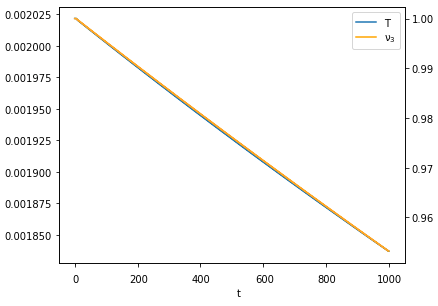
\includegraphics[width=\linewidth]{content/pic/new/impact/impact_1_Tnu3_long.png}
            \vspace{-25pt}
            \caption{Кинетическая энергия $T$ всей системы и угловая скорость $\nu_3$ платформы экипажа на интервале $0 < t < 1000$}
            \label{fig:self_rot_T_long}
        \end{subfigure}
        \begin{subfigure}[t]{\textwidth}
            \vspace{15pt}
            \centering
            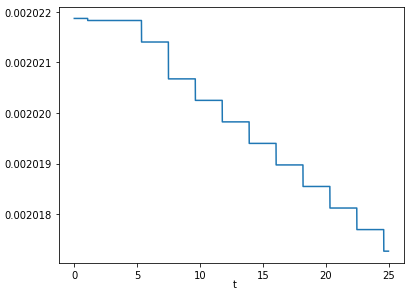
\includegraphics[width=\linewidth]{content/pic/new/impact/impact_1_T.png}
            \vspace{-25pt}
            \caption{Кинетическая энергия $T$ всей системы на интервале $0 < t < 25$}
            \label{fig:self_rot_T}
        \end{subfigure}
    \endminipage
    \quad
    \minipage{0.45\textwidth}
        \vspace{-20pt}
        \begin{subfigure}[t]{\textwidth}
            \centering
            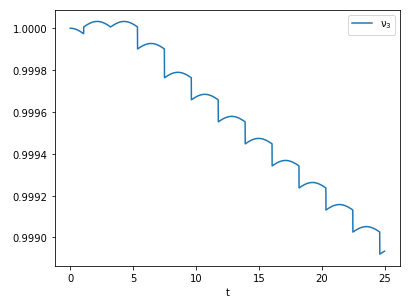
\includegraphics[width=\linewidth]{content/pic/new/impact/impact_1_nu3.png}
            \vspace{-25pt}
            \caption{Угловая скорость $\nu_3$ платформы экипажа}
            \label{fig:self_rot_nu3}
        \end{subfigure}
        \begin{subfigure}[t]{\textwidth}
            \vspace{20pt}
            \centering
            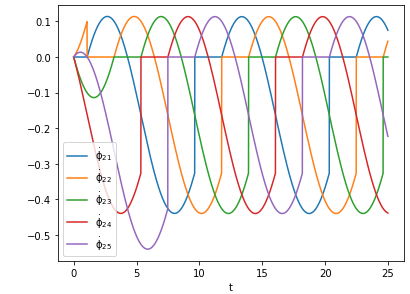
\includegraphics[width=\linewidth]{content/pic/new/impact/impact_1_dphi.png}
            \vspace{-25pt}
            \caption{Угловые скорости роликов на колесе 1.}
            \label{fig:self_rot_dphi}
        \end{subfigure}
    \endminipage

    \caption{Движение 1 ($\nu_{1,2}(0) = 0, \nu_3(0) = 1$) экипажа на абсолютно шероховатой плоскости.}
    \label{fig:self_rot}
\end{figure}

% \begin{figure}[ht]
%     \subf{0.3\textwidth}{
%         \centering
%         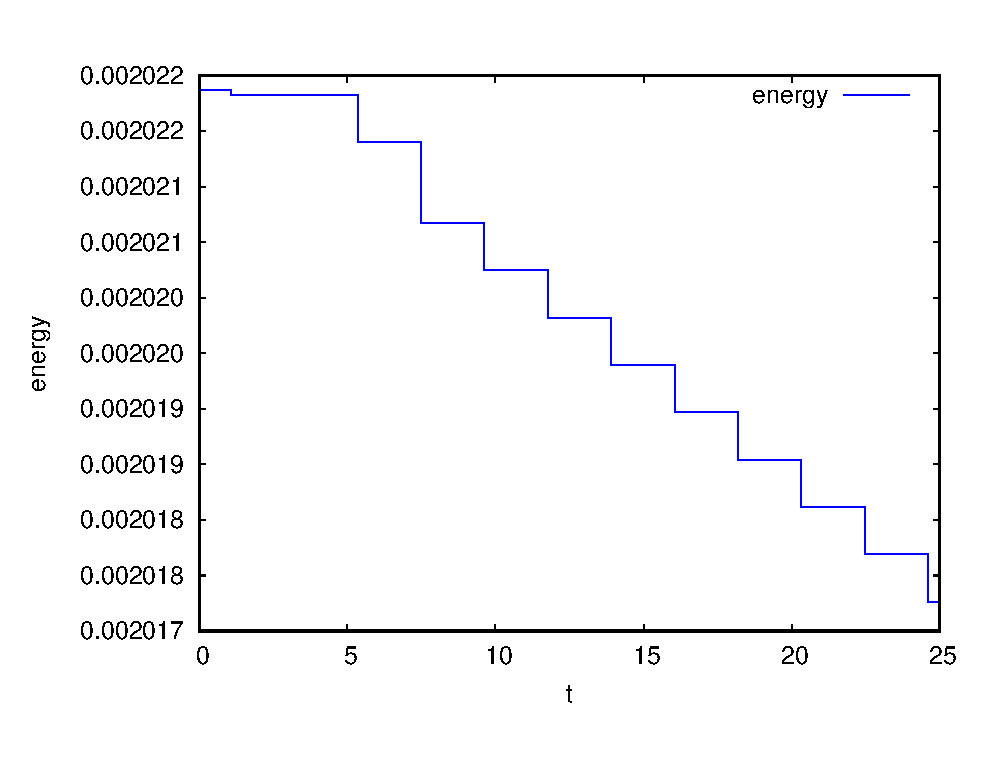
\includegraphics[scale=0.33]{content/pic/self_rot_25/kin_en.eps}
%         \caption{Кинетическая энергия}
%         \label{fig:self_rot_25_kin_en}
%     }
%     \hspace{10pt}
%     \subf{0.3\textwidth}{
%         \centering
%         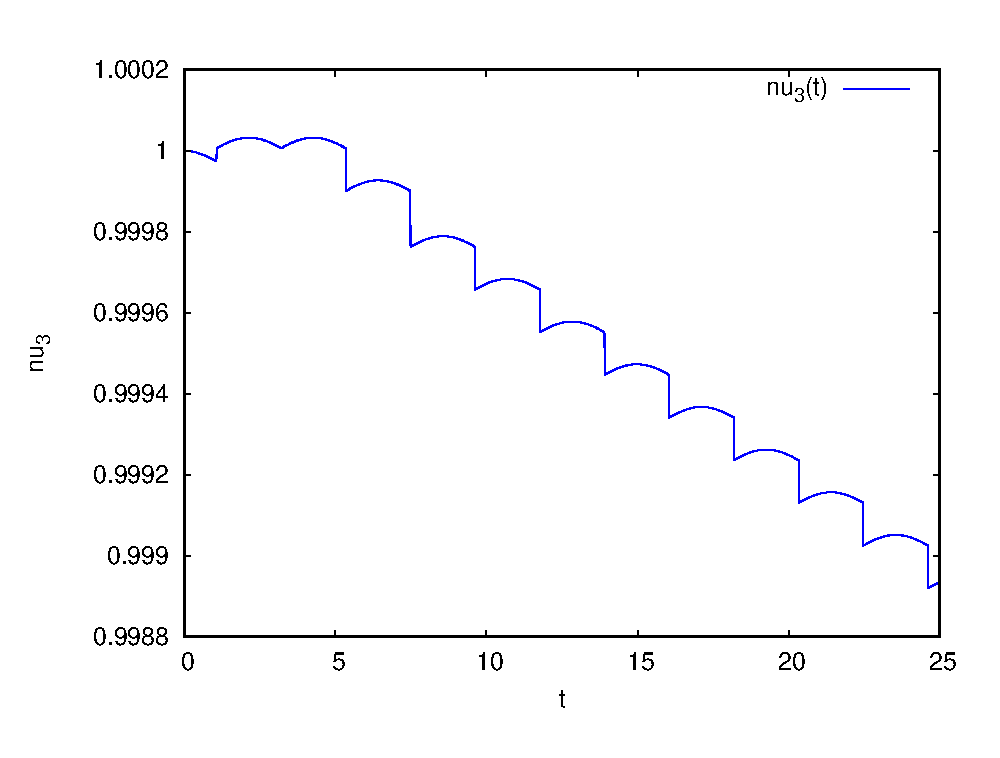
\includegraphics[scale=0.33]{content/pic/self_rot_25/nu3.eps}
%         \caption{Угловая скорость экипажа}
%         \label{fig:self_rot_25_nu3}
%     }
%     \hspace{10pt}
%     \subf{0.3\textwidth}{
%         \centering
%         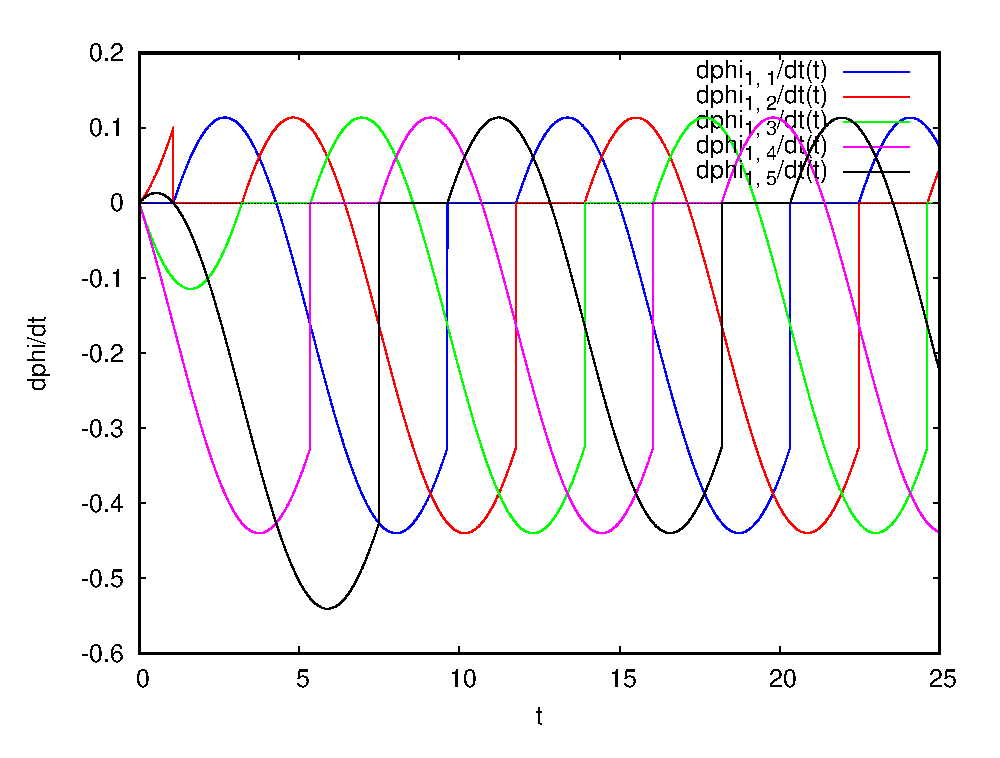
\includegraphics[scale=0.33]{content/pic/self_rot_25/rol_vel.eps}
%         \caption{Угловые скорости роликов}
%         \label{fig:self_rot_25_rol_vel}
%     }
%     \newline
%     \subf{0.3\textwidth}{
%         \centering
%         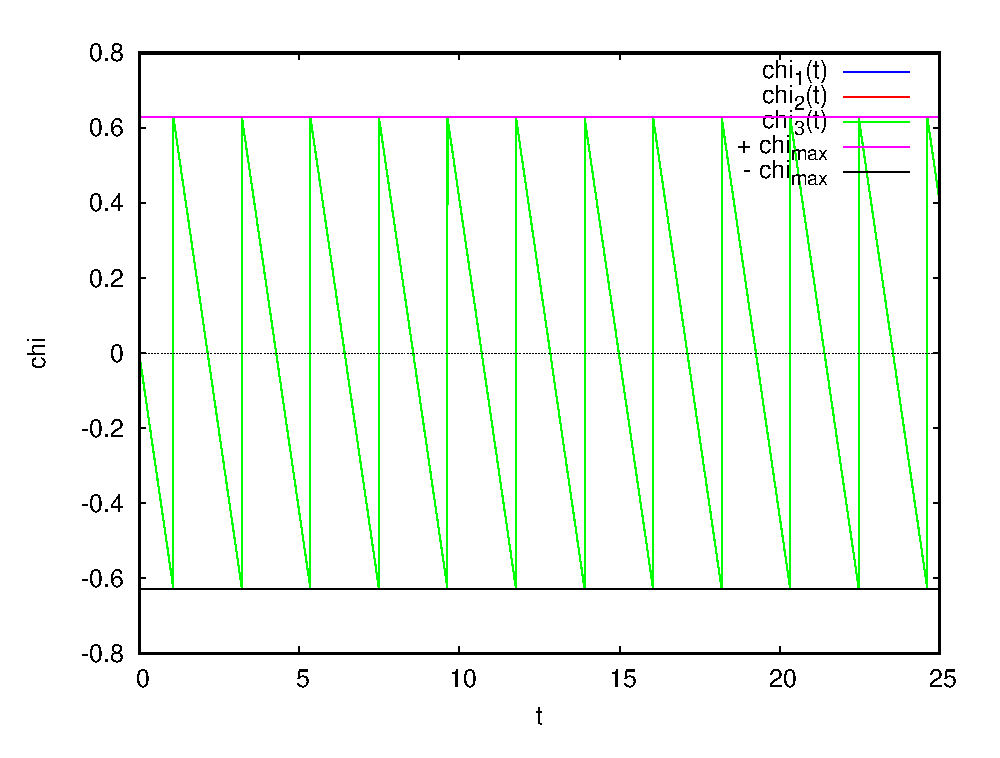
\includegraphics[scale=0.33]{content/pic/self_rot_25/chi.eps}
%         \caption{Углы поворота колес}
%         \label{fig:self_rot_25_chi}
%     }
%     \hspace{10pt}
%     \subf{0.3\textwidth}{
%         \centering
%         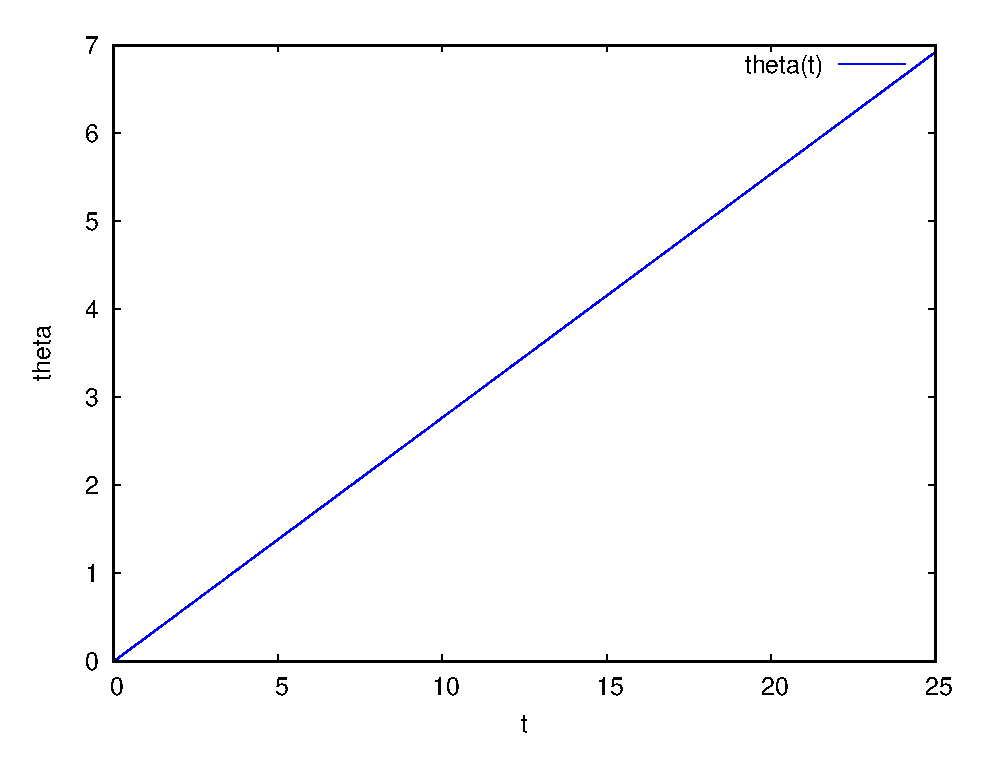
\includegraphics[scale=0.33]{content/pic/self_rot_25/theta.eps}
%         \caption{Угол поворота экипажа}
%         \label{fig:self_rot_25_theta}
%     }
%     \hspace{10pt}
%     \subf{0.3\textwidth}{
%         \centering
%         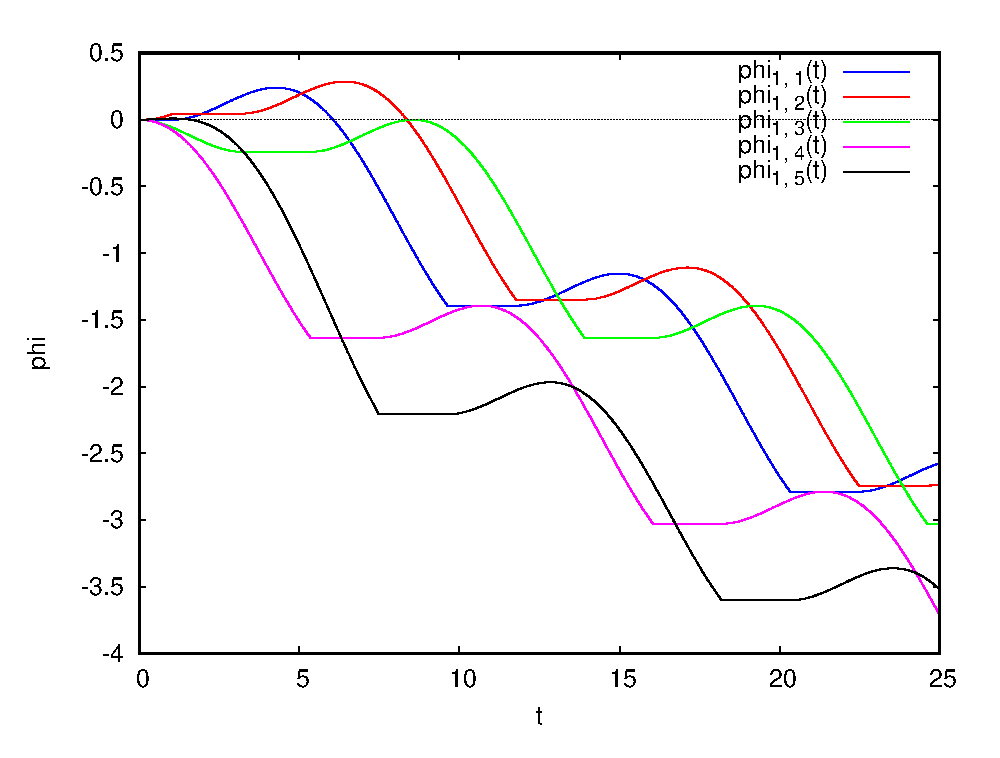
\includegraphics[scale=0.33]{content/pic/self_rot_25/rol_ang.eps}
%         \caption{Углы поворота роликов}
%         \label{fig:self_rot_25_rol_ang}
%     }
%     \caption{Вращение экипажа вокруг своей оси}
%     \label{fig:self_rot}
% \end{figure}

\newpage

% \subsection{По прямой}

\begin{figure}[htb]
    \centering
    \minipage{0.45\textwidth}
        \begin{subfigure}[t]{\textwidth}
            \centering
            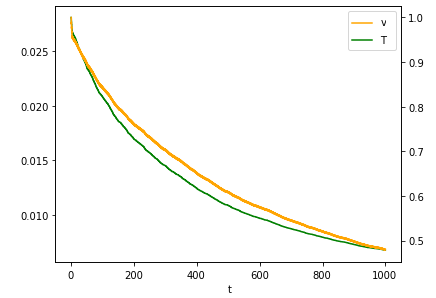
\includegraphics[width=\linewidth]{content/pic/new/impact/impact_2_Tv_long.png}
            \vspace{-25pt}
            \caption{Абсолютная величина $v$ скорости центра масс экипажа и кинетическая энергия $T$ всей системы на интервале $0 < t < 1000$}
            \label{fig:straight_Tv_long}
        \end{subfigure}
        \begin{subfigure}[t]{\textwidth}
            \vspace{15pt}
            \centering
            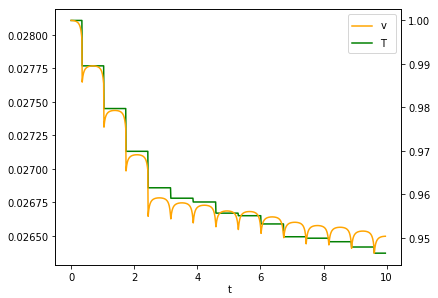
\includegraphics[width=\linewidth]{content/pic/new/impact/impact_2_Tv.png}
            \vspace{-25pt}
            \caption{Абсолютная величина $v$ скорости центра масс экипажа и кинетическая энергия $T$ всей системы на интервале $0 < t < 10$}
            \label{fig:straight_Tv}
        \end{subfigure}
    \endminipage
    \quad
    \minipage{0.45\textwidth}
        \vspace{-20pt}
        \begin{subfigure}[t]{\textwidth}
            \centering
            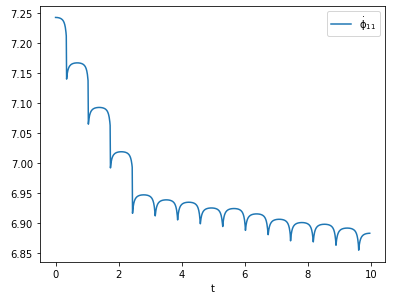
\includegraphics[width=\linewidth]{content/pic/new/impact/impact_2_dphi_1.png}
            \vspace{-25pt}
            \caption{Угловая скорость собственного вращения ролика с номером $1$ на переднем колесе}
            \label{fig:straight_dphi_1}
        \end{subfigure}
        \begin{subfigure}[t]{\textwidth}
            \vspace{20pt}
            \centering
            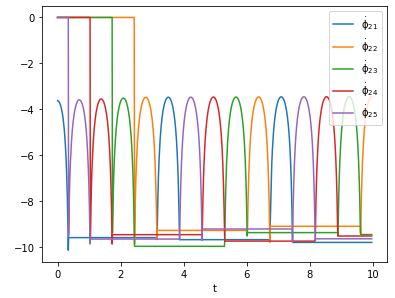
\includegraphics[width=\linewidth]{content/pic/new/impact/impact_2_dphi_2.png}
            \vspace{-25pt}
            \caption{Угловые скорости роликов на колесе номер 2 (одном из задних).}
            \label{fig:straight_dphi_2}
        \end{subfigure}
    \endminipage

    \caption{Движение 2 ($\nu_{1}(0) = 1, \nu_{2,3}(0) = 0$) экипажа на абсолютно шероховатой плоскости.}
    \label{fig:straight}
\end{figure}

% \begin{figure}[ht]
%     \hspace{-20pt}
%     \subf{0.22\textwidth}{
%         \centering
%         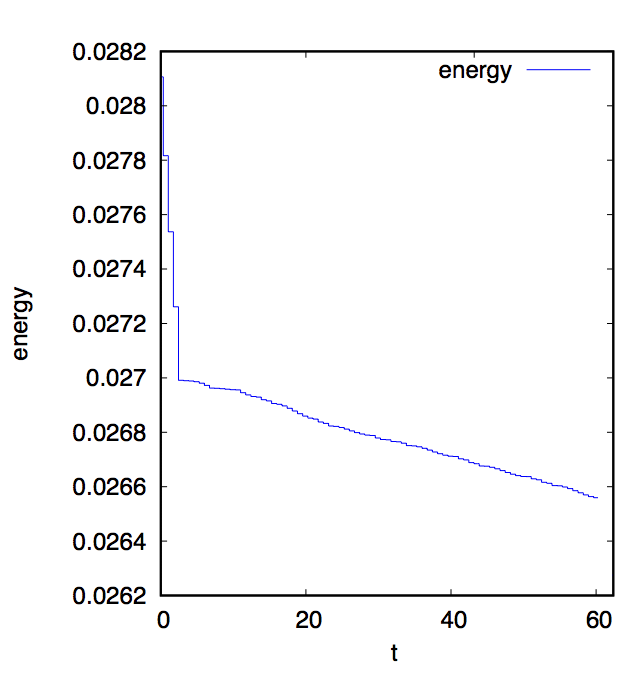
\includegraphics[scale=0.22]{content/pic/straight_60/kin_en.png}
%         \caption{Кинетическая энергия}
%         \label{fig:straight_60_kin_en}
%     }
%     \hspace{20pt}
%     \subf{0.4\textwidth}{
%         \centering
%         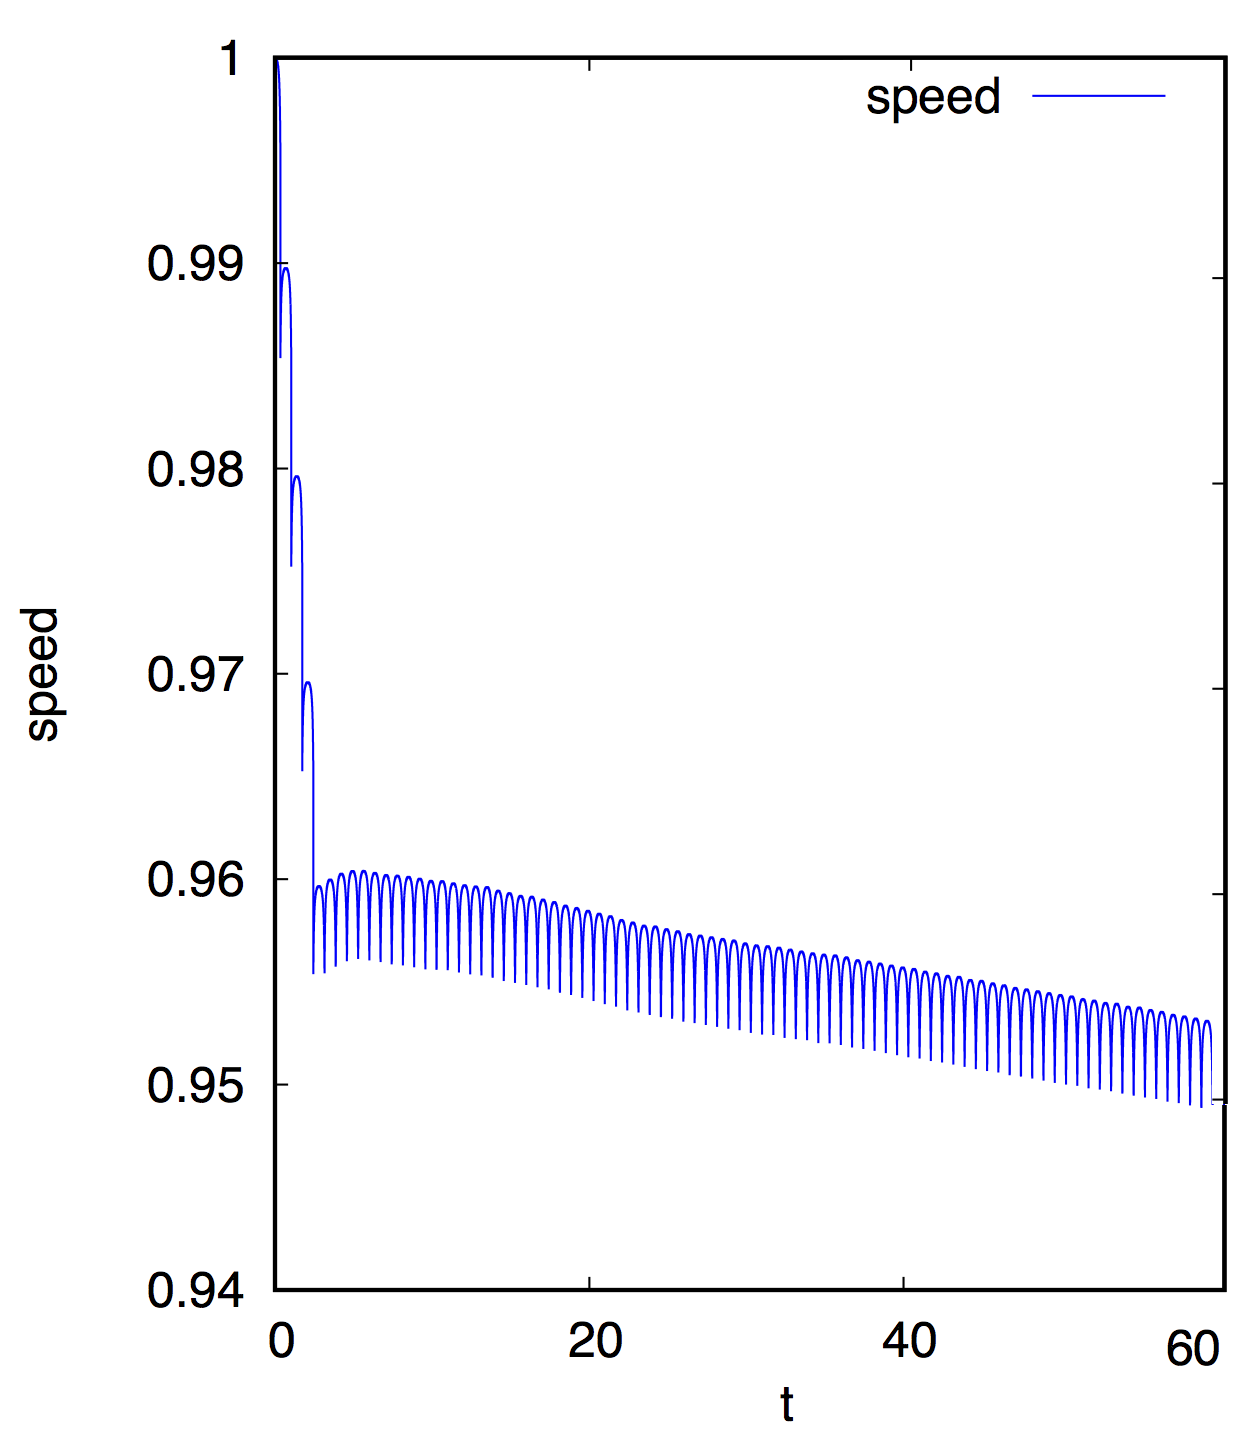
\includegraphics[scale=0.43]{content/pic/straight_60/v.png}
%         \caption{Скорость центра масс}
%         \label{fig:straight_60_v}
%     }
%     % \hspace{10pt}
%     \subf{0.35\textwidth}{
%         \centering
%         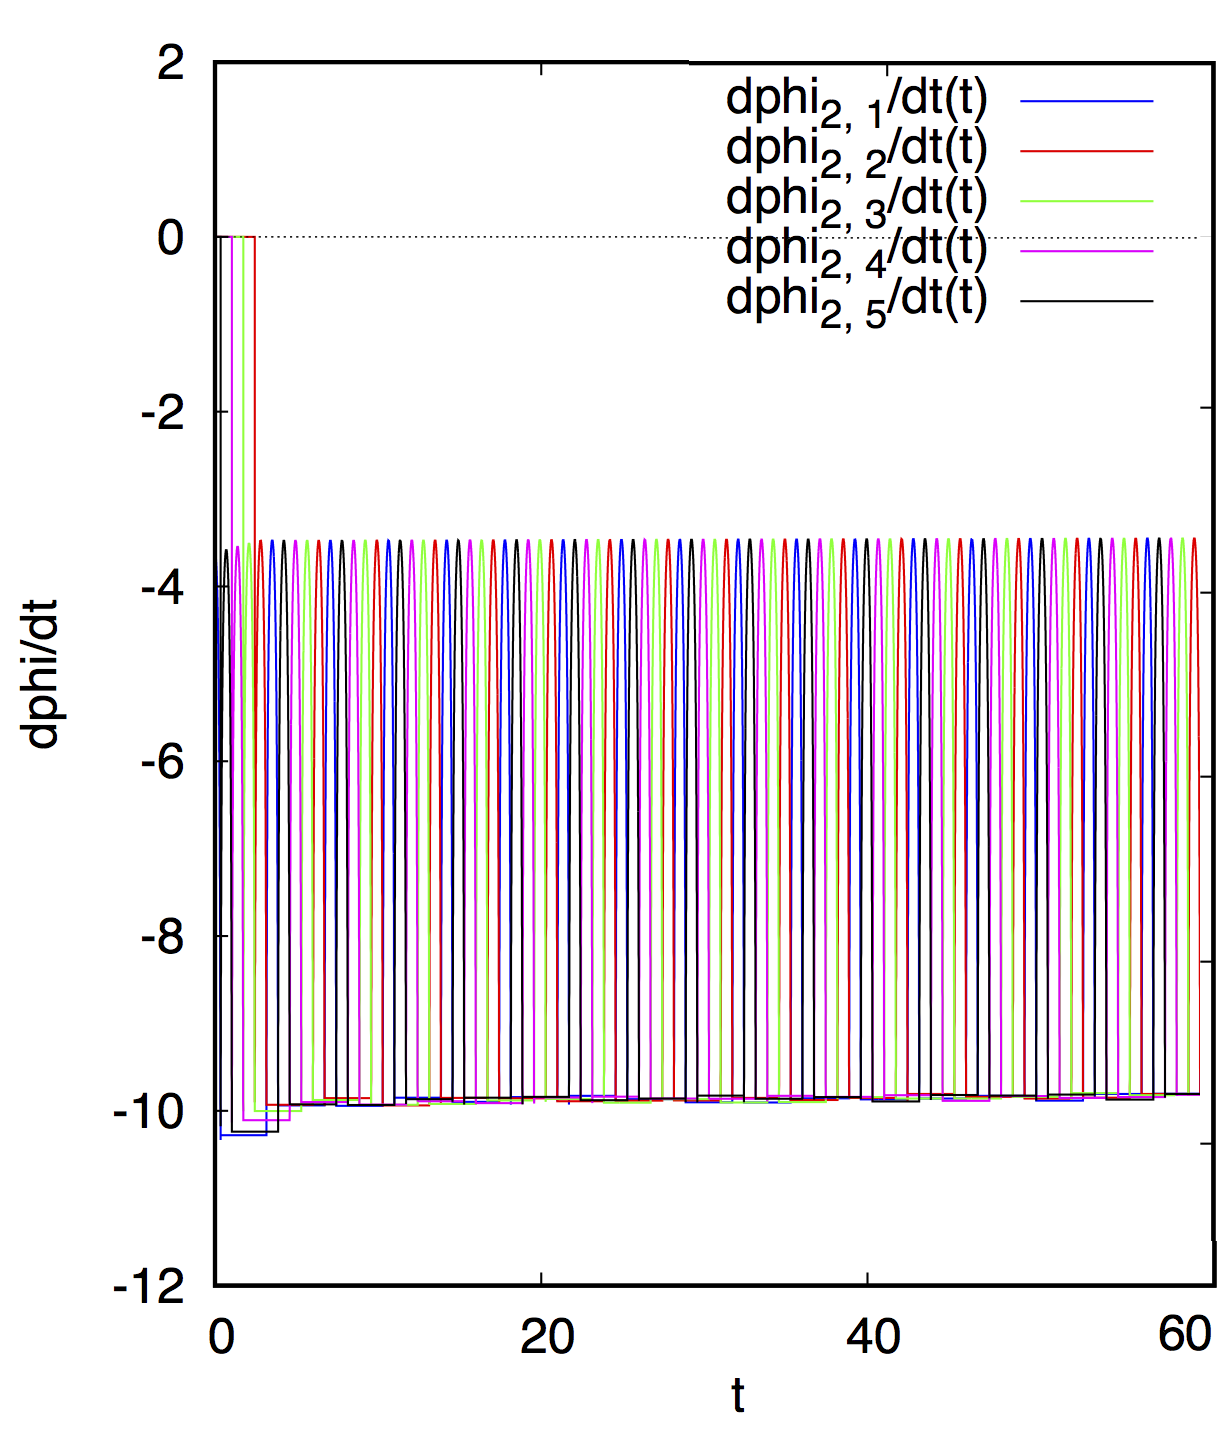
\includegraphics[scale=0.38]{content/pic/straight_60/nus2.png}
%         \caption{Угловые скорости роликов на заднем колесе}
%         \label{fig:straight_60_nus2}
%     }
%     \newline
%     \subf{0.3\textwidth}{
%         \centering
%         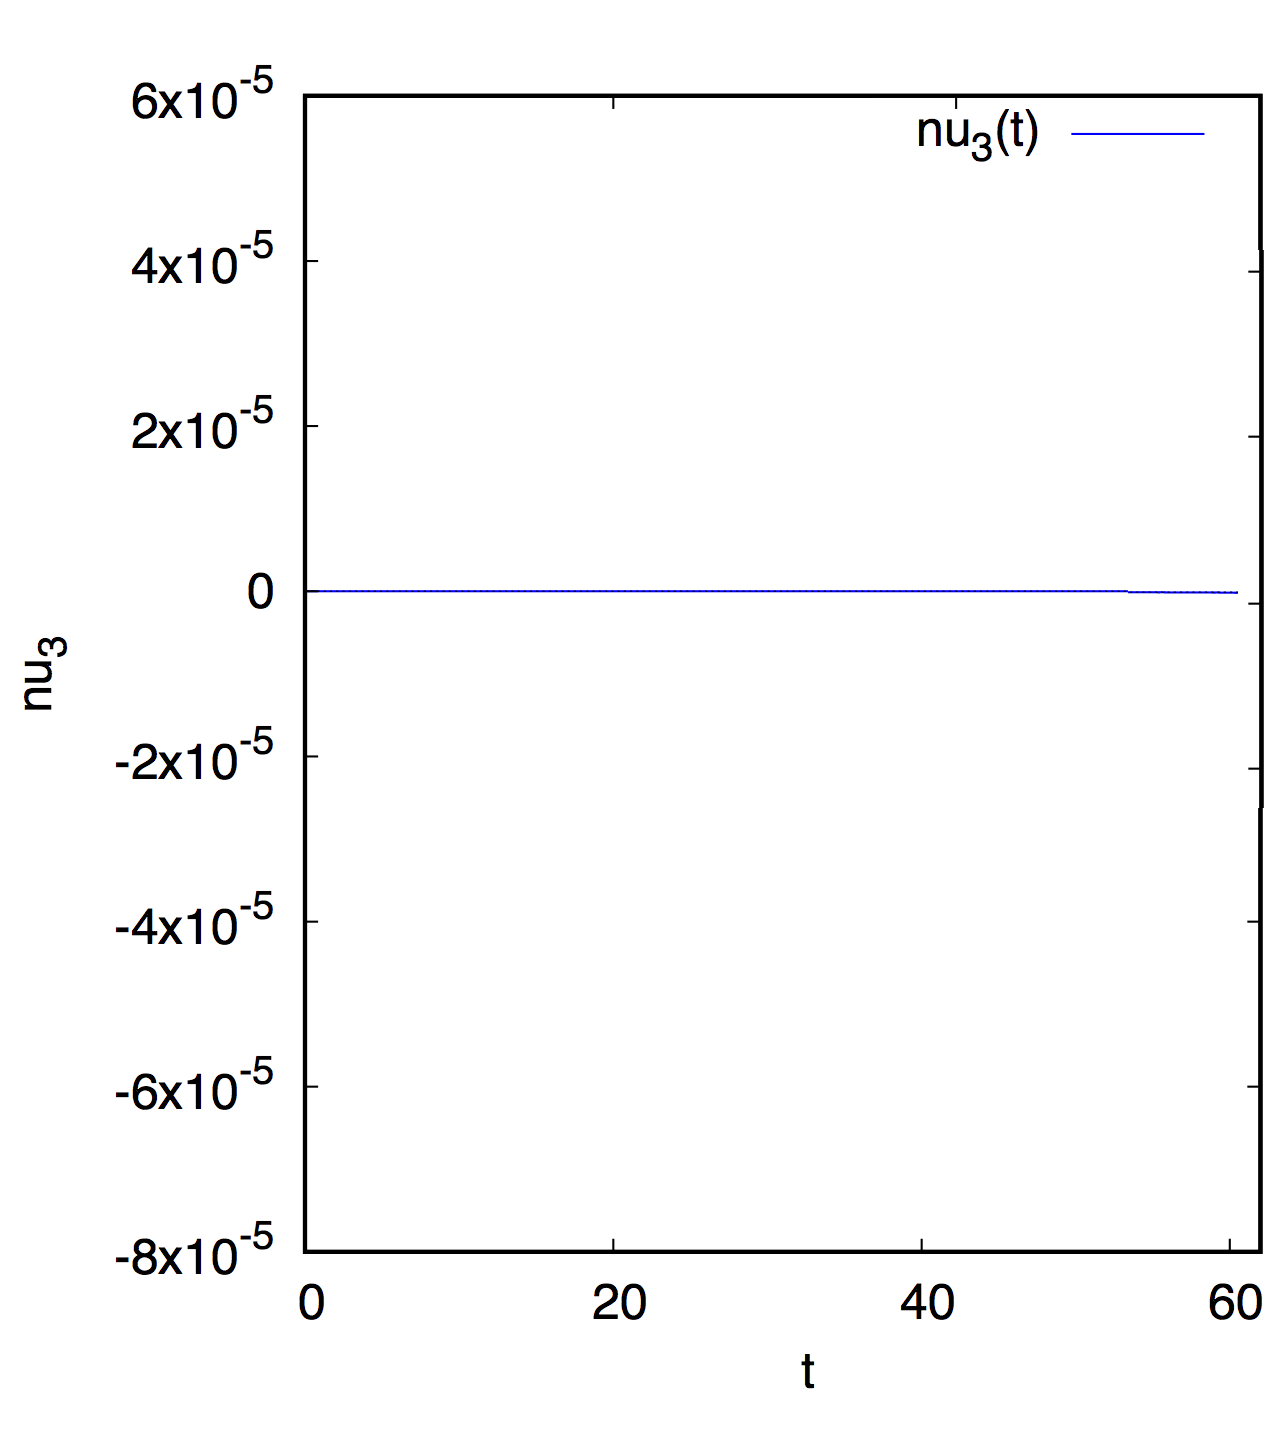
\includegraphics[scale=0.36]{content/pic/straight_60/nu3.png}
%         \caption{Угловая скорость экипажа}
%         \label{fig:straight_60_nu3}
%     }
%     \hspace{10pt}
%     \subf{0.3\textwidth}{
%         \centering
%         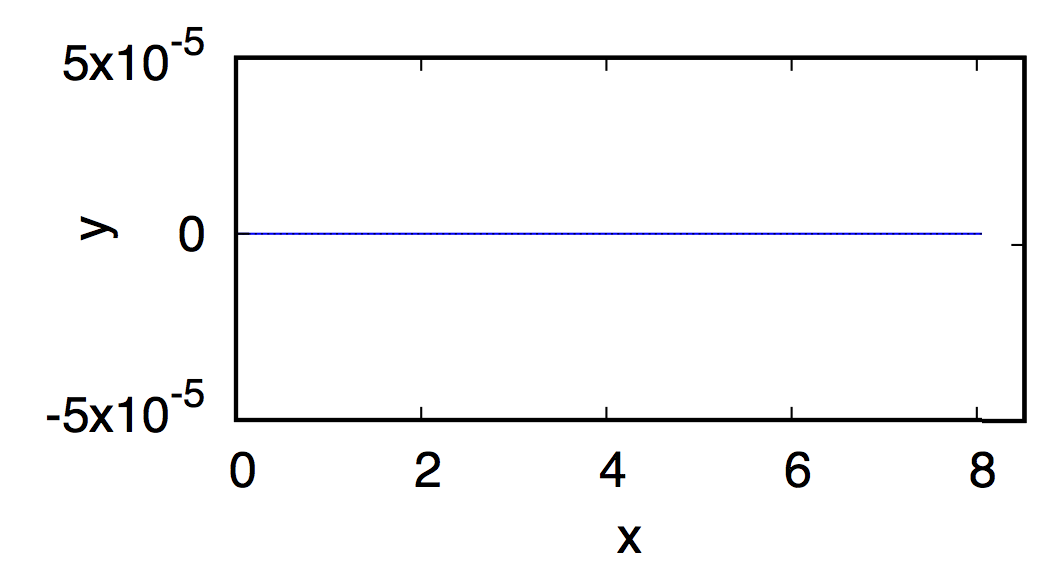
\includegraphics[scale=0.55]{content/pic/straight_60/traj.png}
%         \caption{Траектория}
%         \label{fig:straight_60_traj}
%     }
%     \hspace{10pt}
%     \subf{0.3\textwidth}{
%         \centering
%         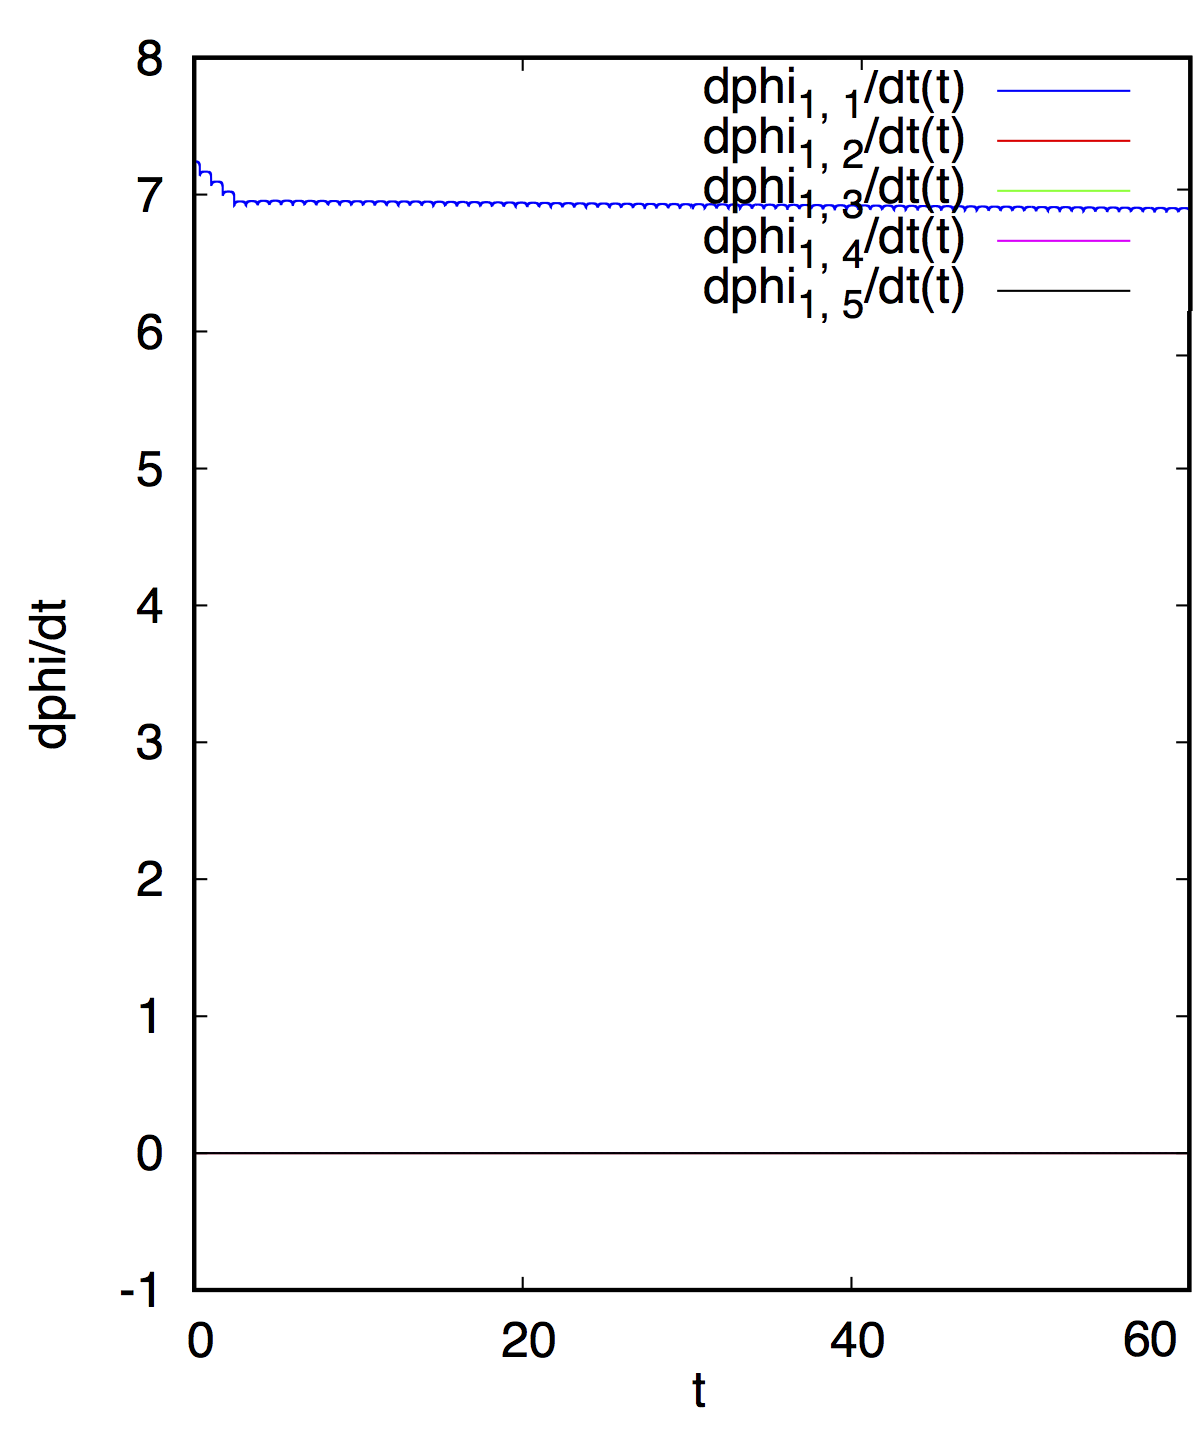
\includegraphics[scale=0.33]{content/pic/straight_60/nus1.png}
%         \caption{Угловые скорости роликов на переднем колесе}
%         \label{fig:straight_60_nus1}
%     }
%     \newline
%     \subf{0.3\textwidth}{
%         \centering
%         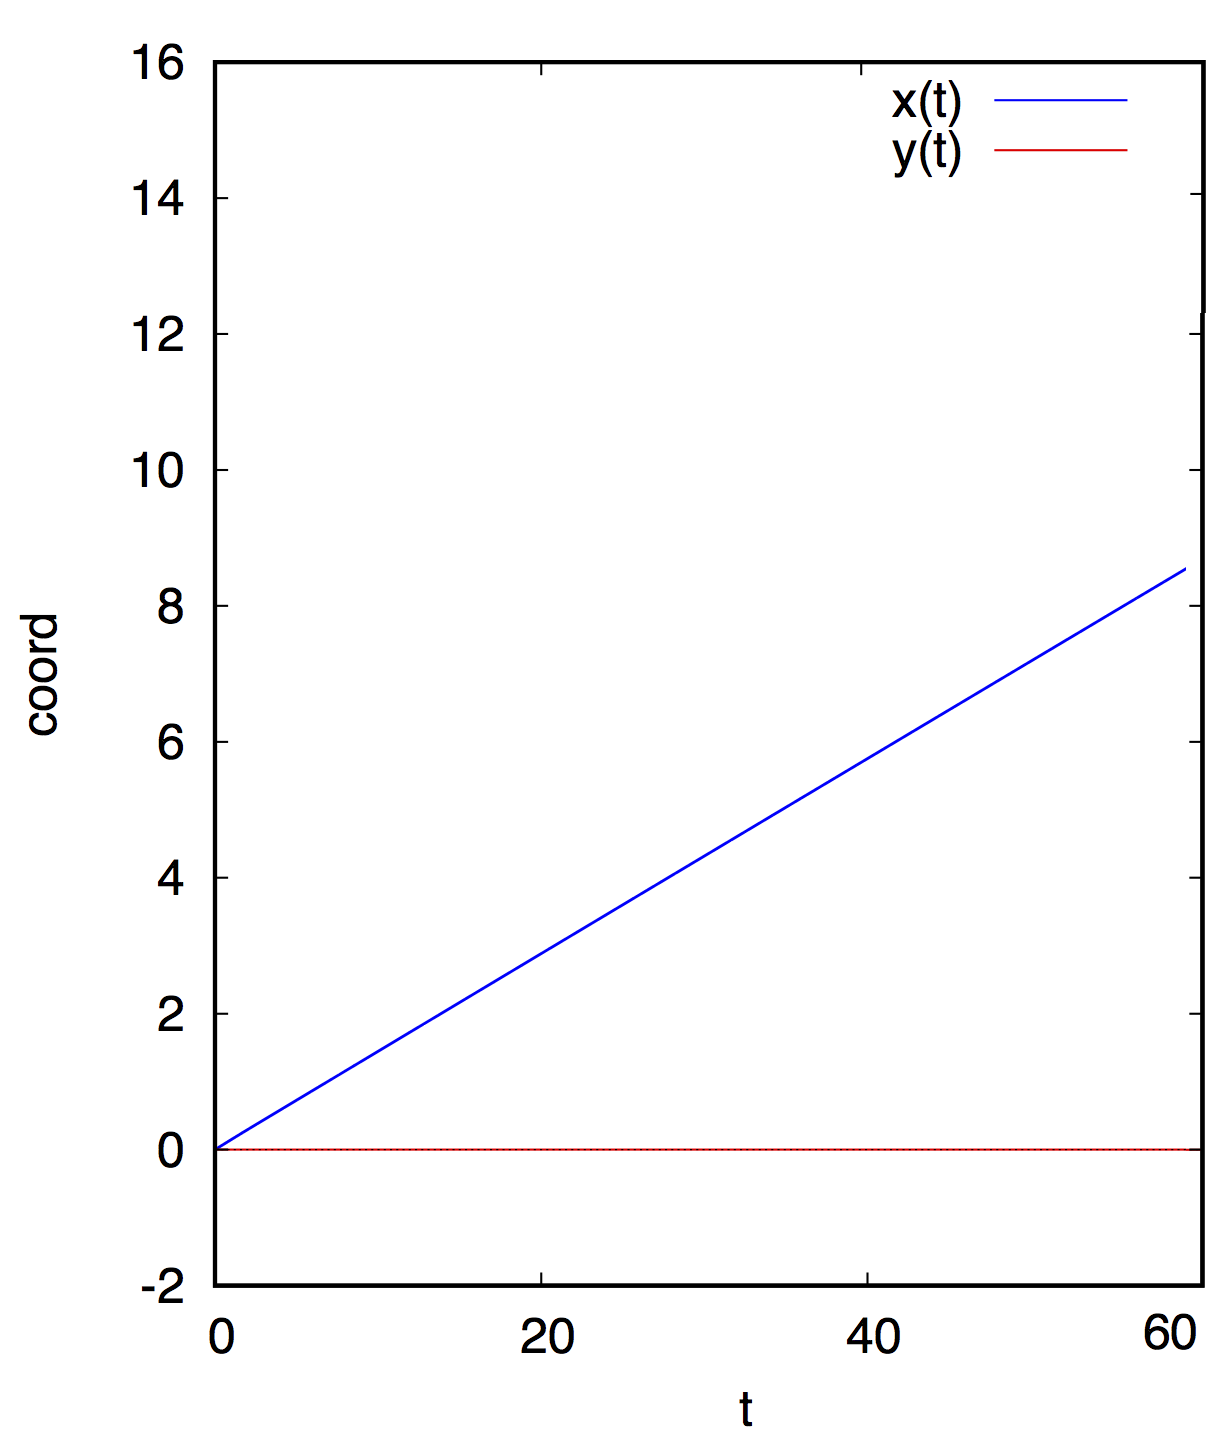
\includegraphics[scale=0.33]{content/pic/straight_60/xy.png}
%         \caption{Координаты центра масс}
%         \label{fig:straight_60_xy}
%     }
%     \hspace{10pt}
%     \subf{0.3\textwidth}{
%         \centering
%         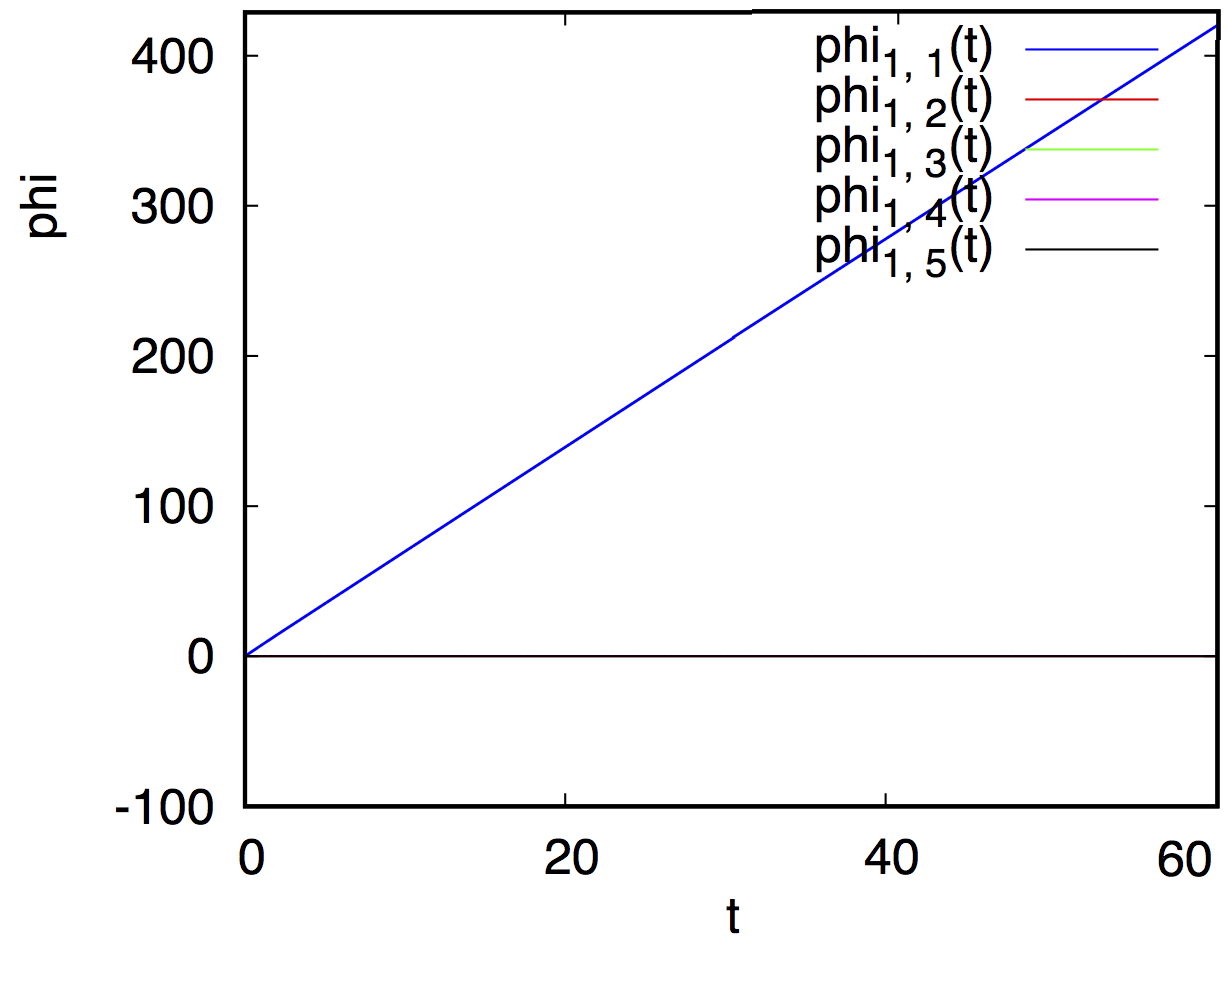
\includegraphics[scale=0.43]{content/pic/straight_60/phi1.png}
%         \caption{Углы поворота роликов на переднем колесе}
%         \label{fig:straight_60_phi1}
%     }
%     \hspace{10pt}
%     \subf{0.3\textwidth}{
%         \centering
%         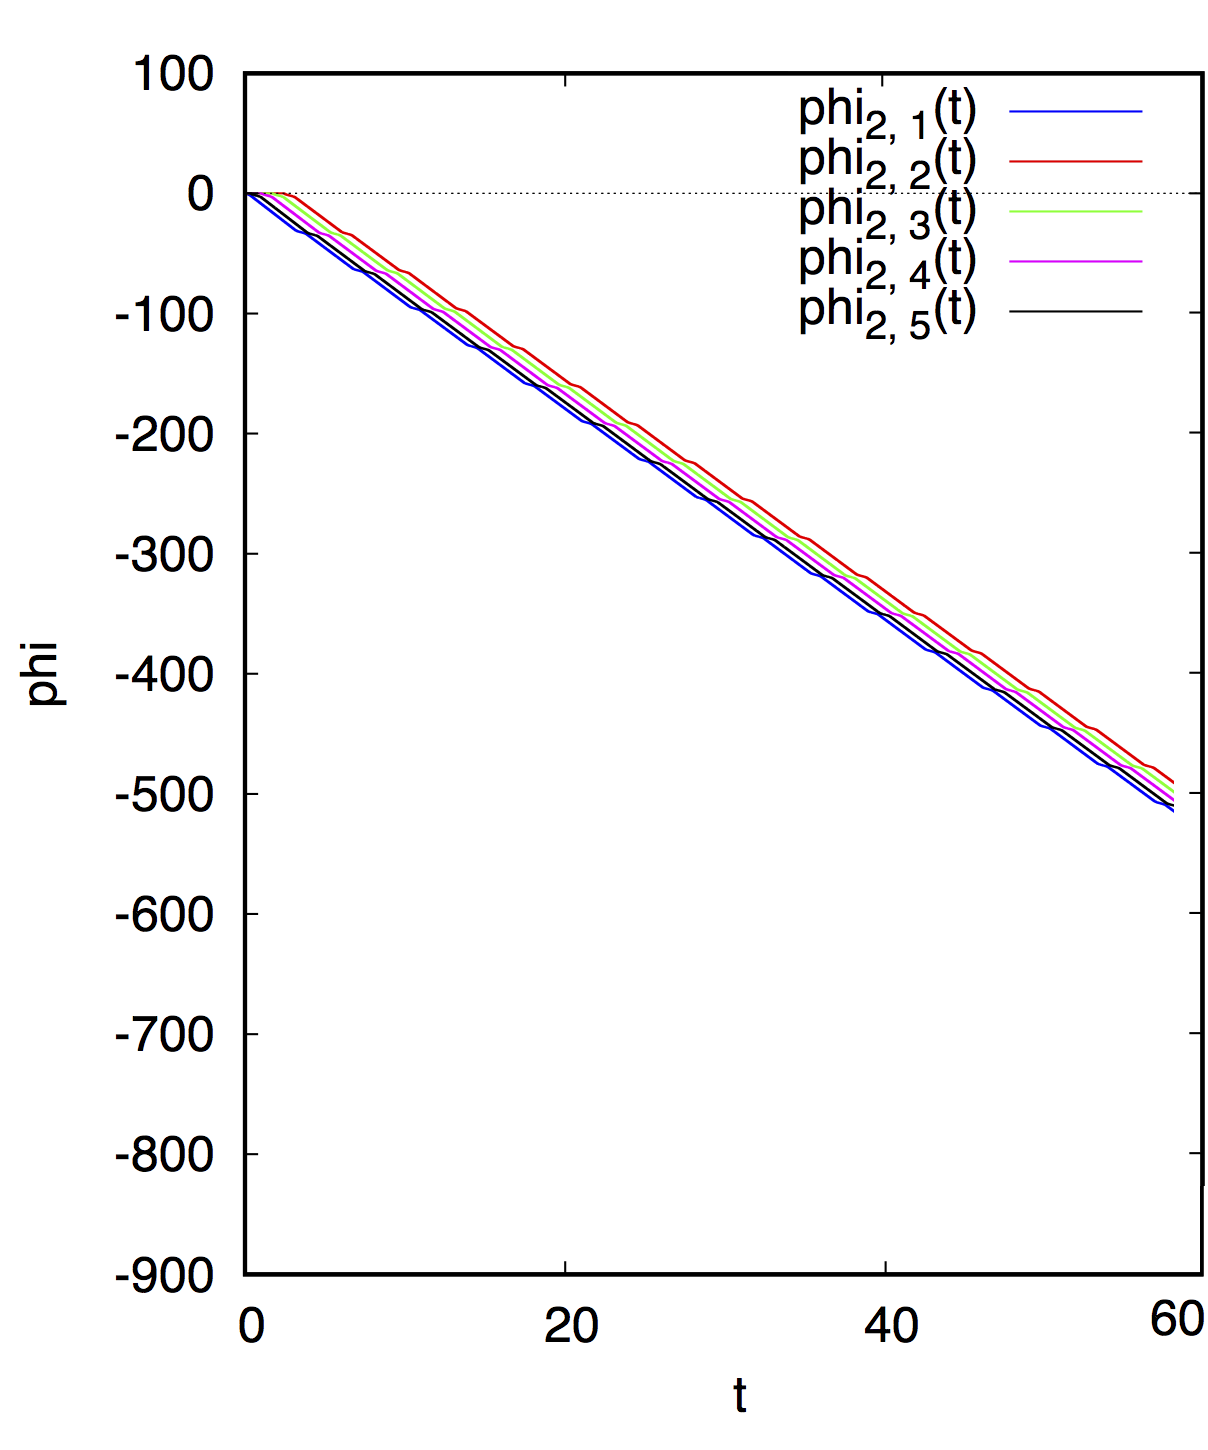
\includegraphics[scale=0.33]{content/pic/straight_60/phi2.png}
%         \caption{Углы поворота роликов на заднем колесе}
%         \label{fig:straight_60_phi2}
%     }
%     \caption{Движение экипажа по прямой}
%     \label{fig:straight}
% \end{figure}

\newpage

% \subsection{С закруткой}

\begin{figure}[htb]
    \centering
    \minipage{0.45\textwidth}
        \begin{subfigure}[t]{\textwidth}
            \centering
            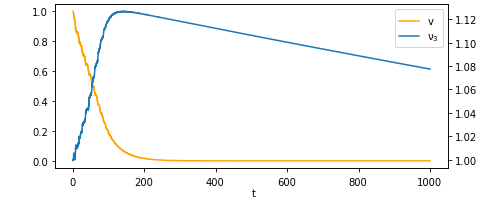
\includegraphics[width=\linewidth]{content/pic/new/impact/impact_3_vnu3.png}
            \vspace{-25pt}
            \caption{Абсолютная величина $v$ скорости центра масс экипажа и угловая скорость платформы $\nu_3$}
            \label{fig:wrench_vnu3}
        \end{subfigure}
        \begin{subfigure}[t]{\textwidth}
            \vspace{15pt}
            \centering
            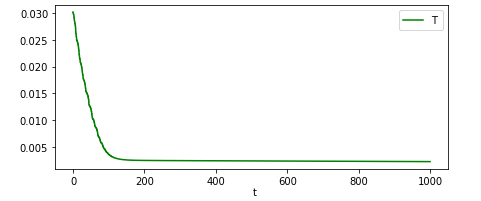
\includegraphics[width=\linewidth]{content/pic/new/impact/impact_3_T.png}
            \vspace{-25pt}
            \caption{Кинетическая энергия экипажа}
            \label{fig:wrench_T}
        \end{subfigure}
        \begin{subfigure}[t]{\textwidth}
            \vspace{15pt}
            \centering
            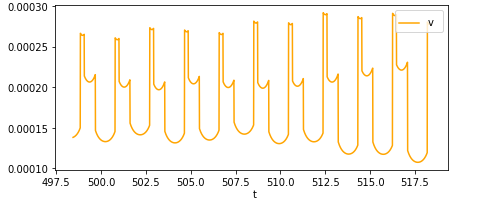
\includegraphics[width=\linewidth]{content/pic/new/impact/impact_3_v_late.png}
            \vspace{-25pt}
            \caption{Абсолютная величина $v$ скорости центра масс экипажа на фрагменте интервала времени после почти полного прекращения поступательного движения центра масс, за исключением показанной величины скорости.}
            \label{fig:wrench_v_late}
        \end{subfigure}
    \endminipage
    \quad
    \minipage{0.45\textwidth}
        \vspace{-35pt}
        \begin{subfigure}[t]{\textwidth}
            \centering
            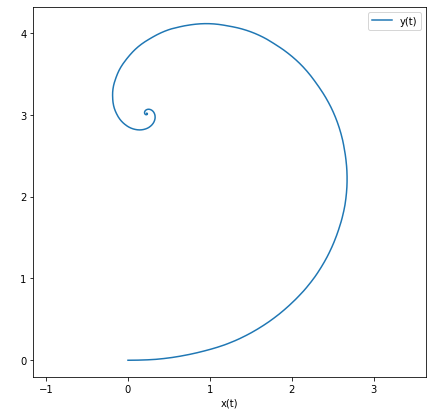
\includegraphics[width=\linewidth]{content/pic/new/impact/impact_3_traj.png}
            \vspace{-25pt}
            \caption{Траектория центра масс экипажа на плоскости $OXY$}
            \label{fig:wrench_traj}
        \end{subfigure}
        \begin{subfigure}[t]{\textwidth}
            \vspace{20pt}
            \centering
            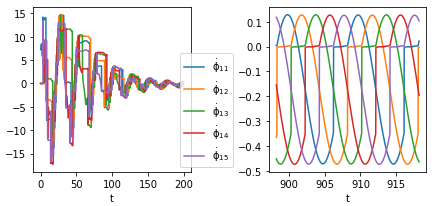
\includegraphics[width=\linewidth]{content/pic/new/impact/impact_3_dphi.png}
            \vspace{-25pt}
            \caption{Угловые скорости роликов на колесе номер 1. Слева -- на интервале $t < 200$, справа -- на фрагменте интервала времени после почти полного прекращения поступательного движения центра масс.}
            \label{fig:wrench_dphi}
        \end{subfigure}
    \endminipage

    \caption{Движение 3 ($\nu_{1}(0) = 1, \nu_{2}(0) = 0, \nu_{3}(0) = 1$) экипажа на абсолютно шероховатой плоскости.}
    \label{fig:wrench}
\end{figure}

% \begin{figure}[ht]
%     \subf{0.3\textwidth}{
%         \centering
%         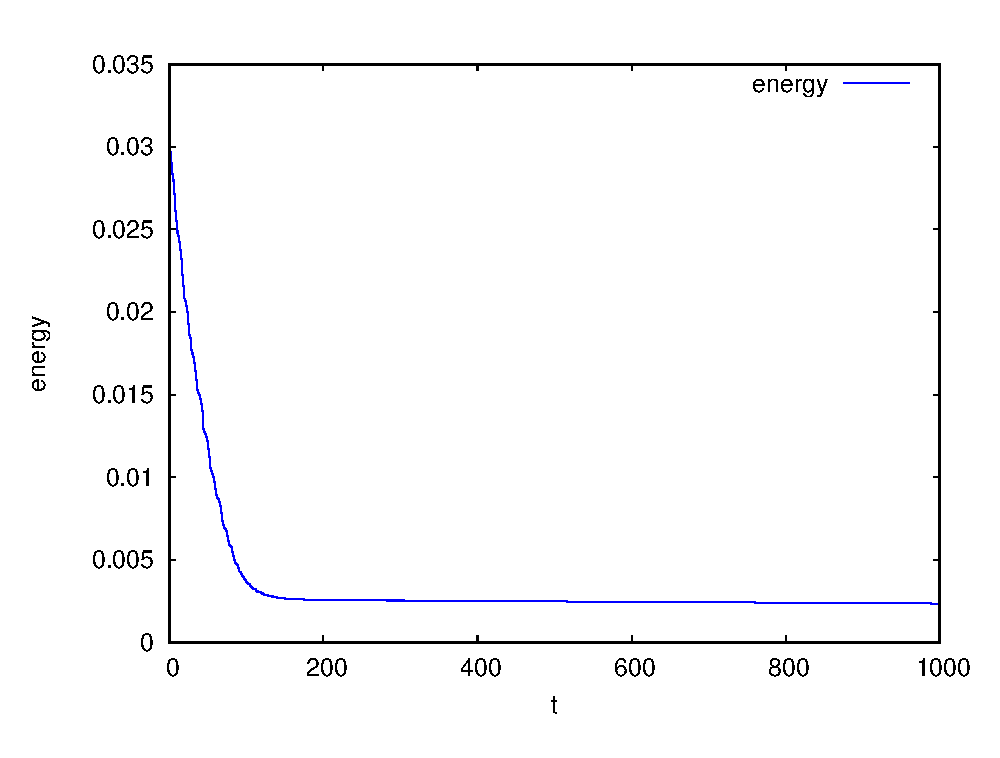
\includegraphics[scale=0.33]{content/pic/wrench_1000/kin_en.eps}
%         \caption{Кинетическая энергия}
%         \label{fig:wrench_1000_kin_en}
%     }
%     \hspace{10pt}
%     \subf{0.3\textwidth}{
%         \centering
%         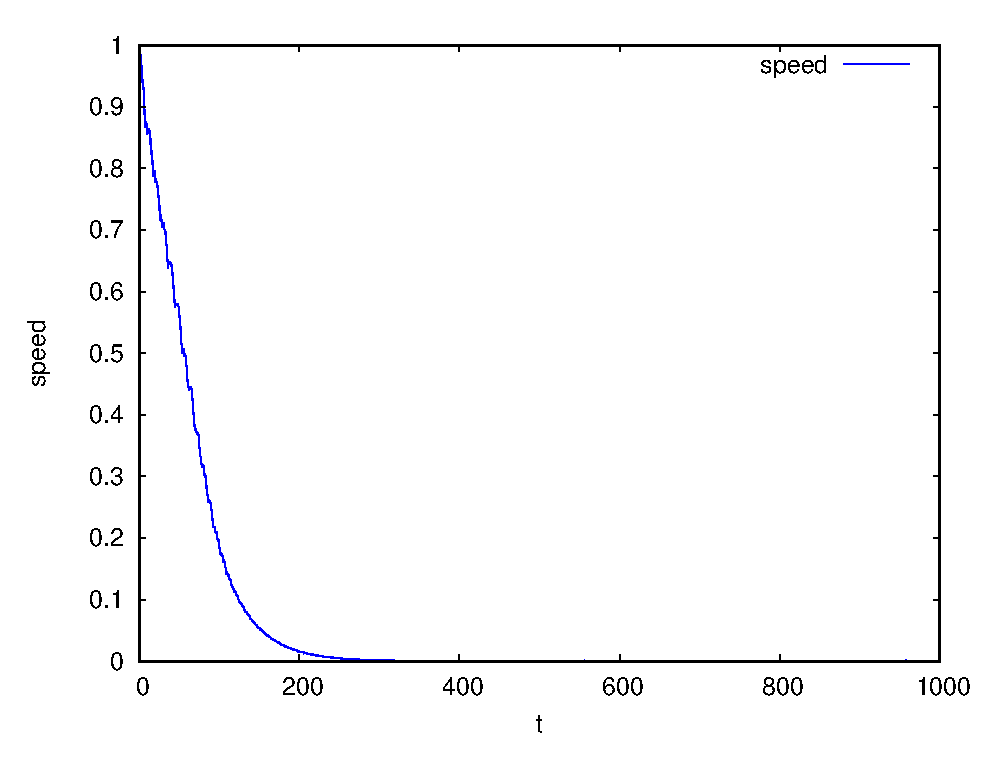
\includegraphics[scale=0.33]{content/pic/wrench_1000/v.eps}
%         \caption{Скорость центра масс}
%         \label{fig:wrench_1000_v}
%     }
%     \hspace{10pt}
%     \subf{0.3\textwidth}{
%         \centering
%         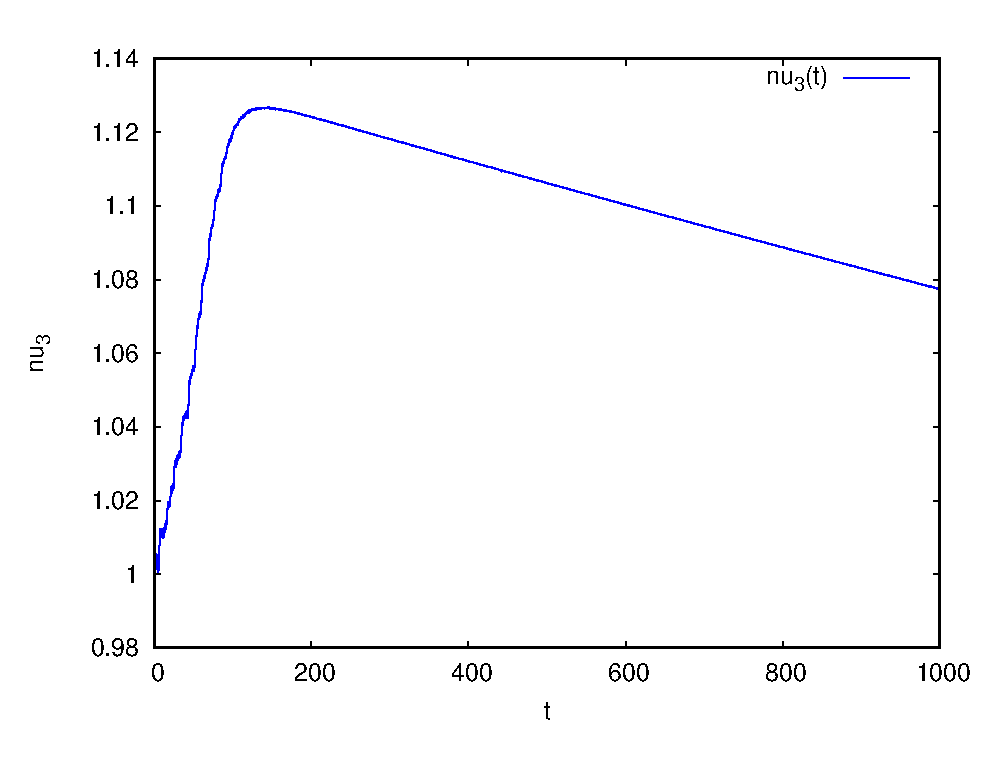
\includegraphics[scale=0.33]{content/pic/wrench_1000/nu3.eps}
%         \caption{Угловая скорость экипажа}
%         \label{fig:wrench_1000_nu3}
%     }
%     \newline
%     \subf{0.45\textwidth}{
%         \centering
%         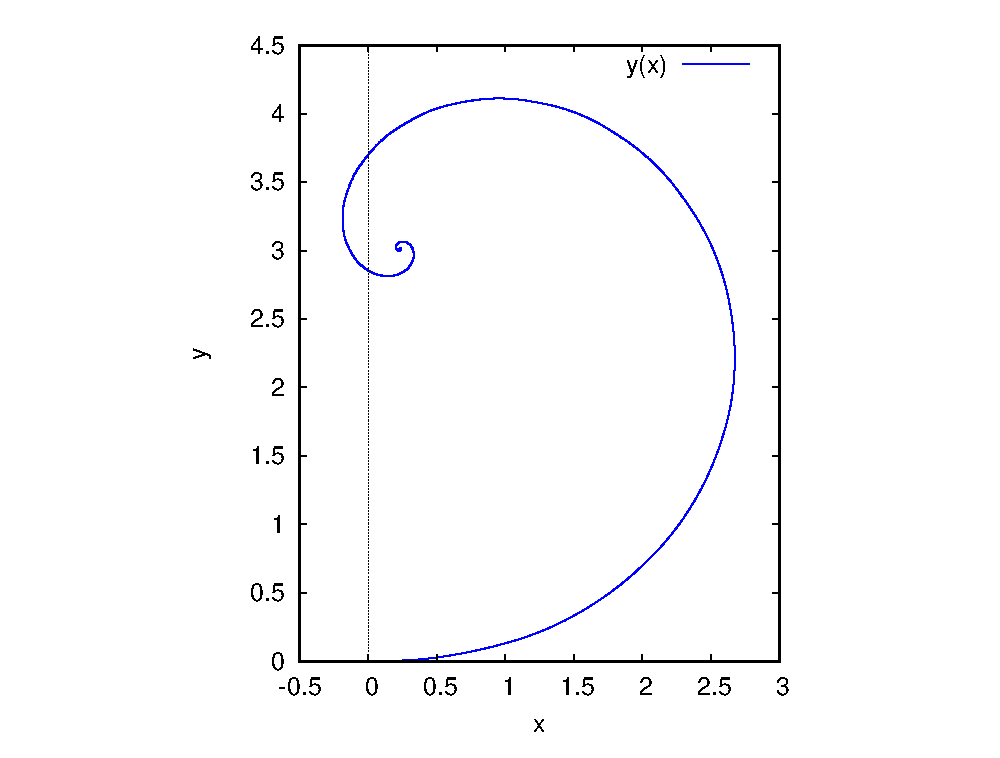
\includegraphics[scale=0.33]{content/pic/wrench_1000/traj.eps}
%         \caption{Траектория центра масс}
%         \label{fig:wrench_1000_traj}
%     }
%     \hspace{10pt}
%     \subf{0.45\textwidth}{
%         \centering
%         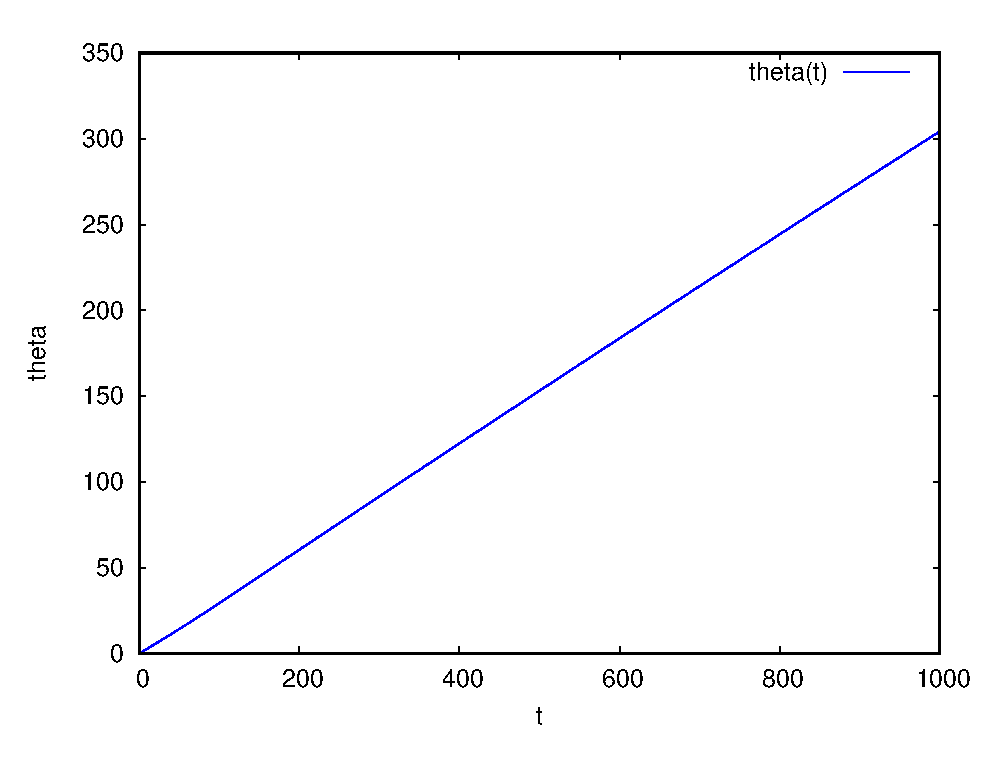
\includegraphics[scale=0.33]{content/pic/wrench_1000/theta.eps}
%         \caption{Угол поворота экипажа}
%         \label{fig:wrench_1000_theta}
%     }
%     \newline
%     \subf{0.45\textwidth}{
%         \centering
%         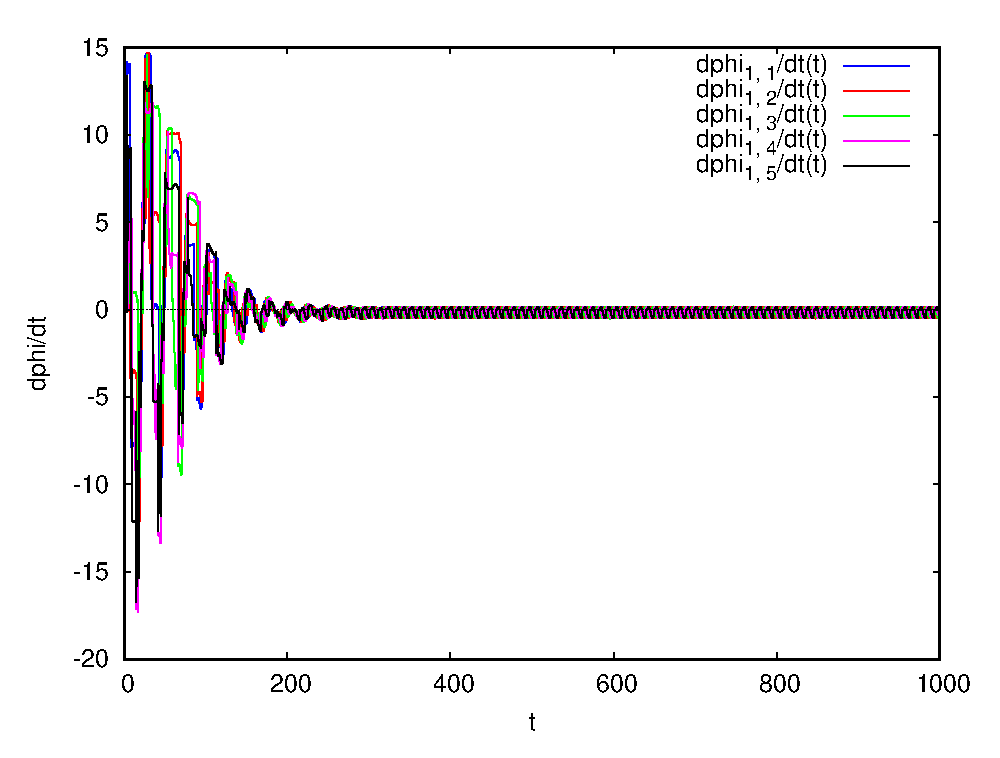
\includegraphics[scale=0.33]{content/pic/wrench_1000/nus1.eps}
%         \caption{Угловые скорости роликов на переднем колесе}
%         \label{fig:wrench_1000_nus1}
%     }
%     \hspace{10pt}
%     \subf{0.45\textwidth}{
%         \centering
%         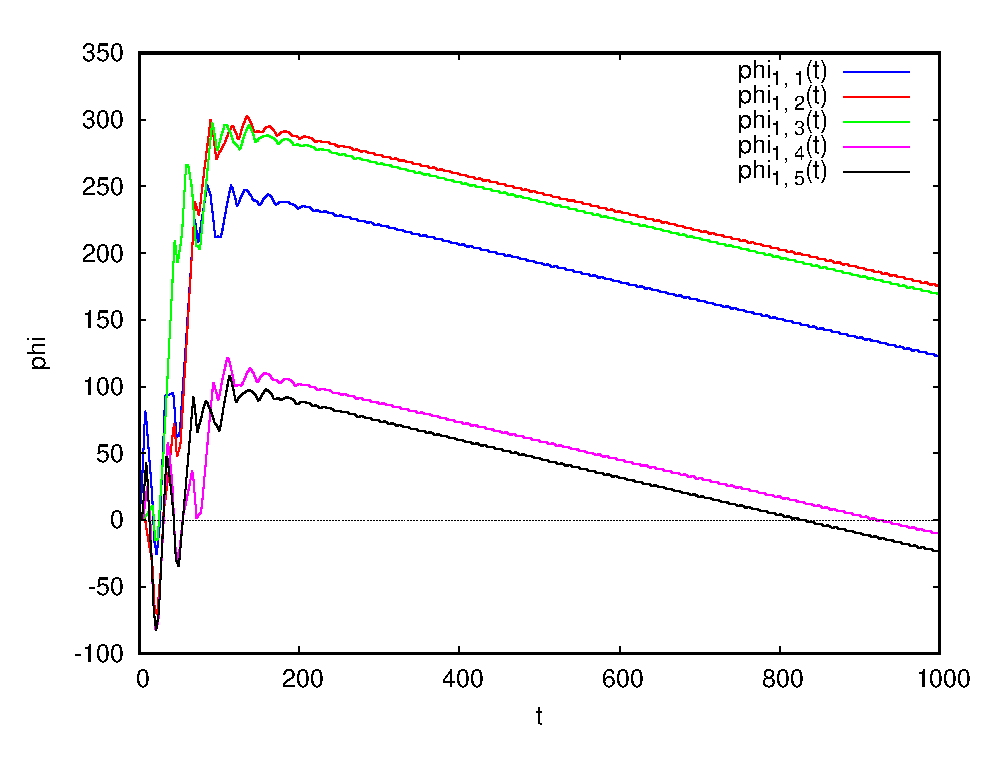
\includegraphics[scale=0.33]{content/pic/wrench_1000/phi1.eps}
%         \caption{Углы поворота роликов на переднем колесе}
%         \label{fig:wrench_1000_phi1}
%     }
%     \caption{Движение экипажа с закруткой}
%     \label{fig:wrench}
% \end{figure}

\newpage

% \chapter[Уравнения движения экипажа на~омни-колесах с~учетом динамики роликов]{Уравнения движения \\ экипажа~на~омни-колесах \\ с~учетом~динамики~роликов}


% \section{Отслеживание контакта и моделирование трения}

Для наглядности мы ограничиваемся рассмотрением омни-колес, 
оснащенных четырьмя роликами. Также для простоты сами ролики имеют оси 
вращения, лежащие в плоскости колеса (Рис.~\ref{OmniWheel}).

\begin{figure}[htb]
\centering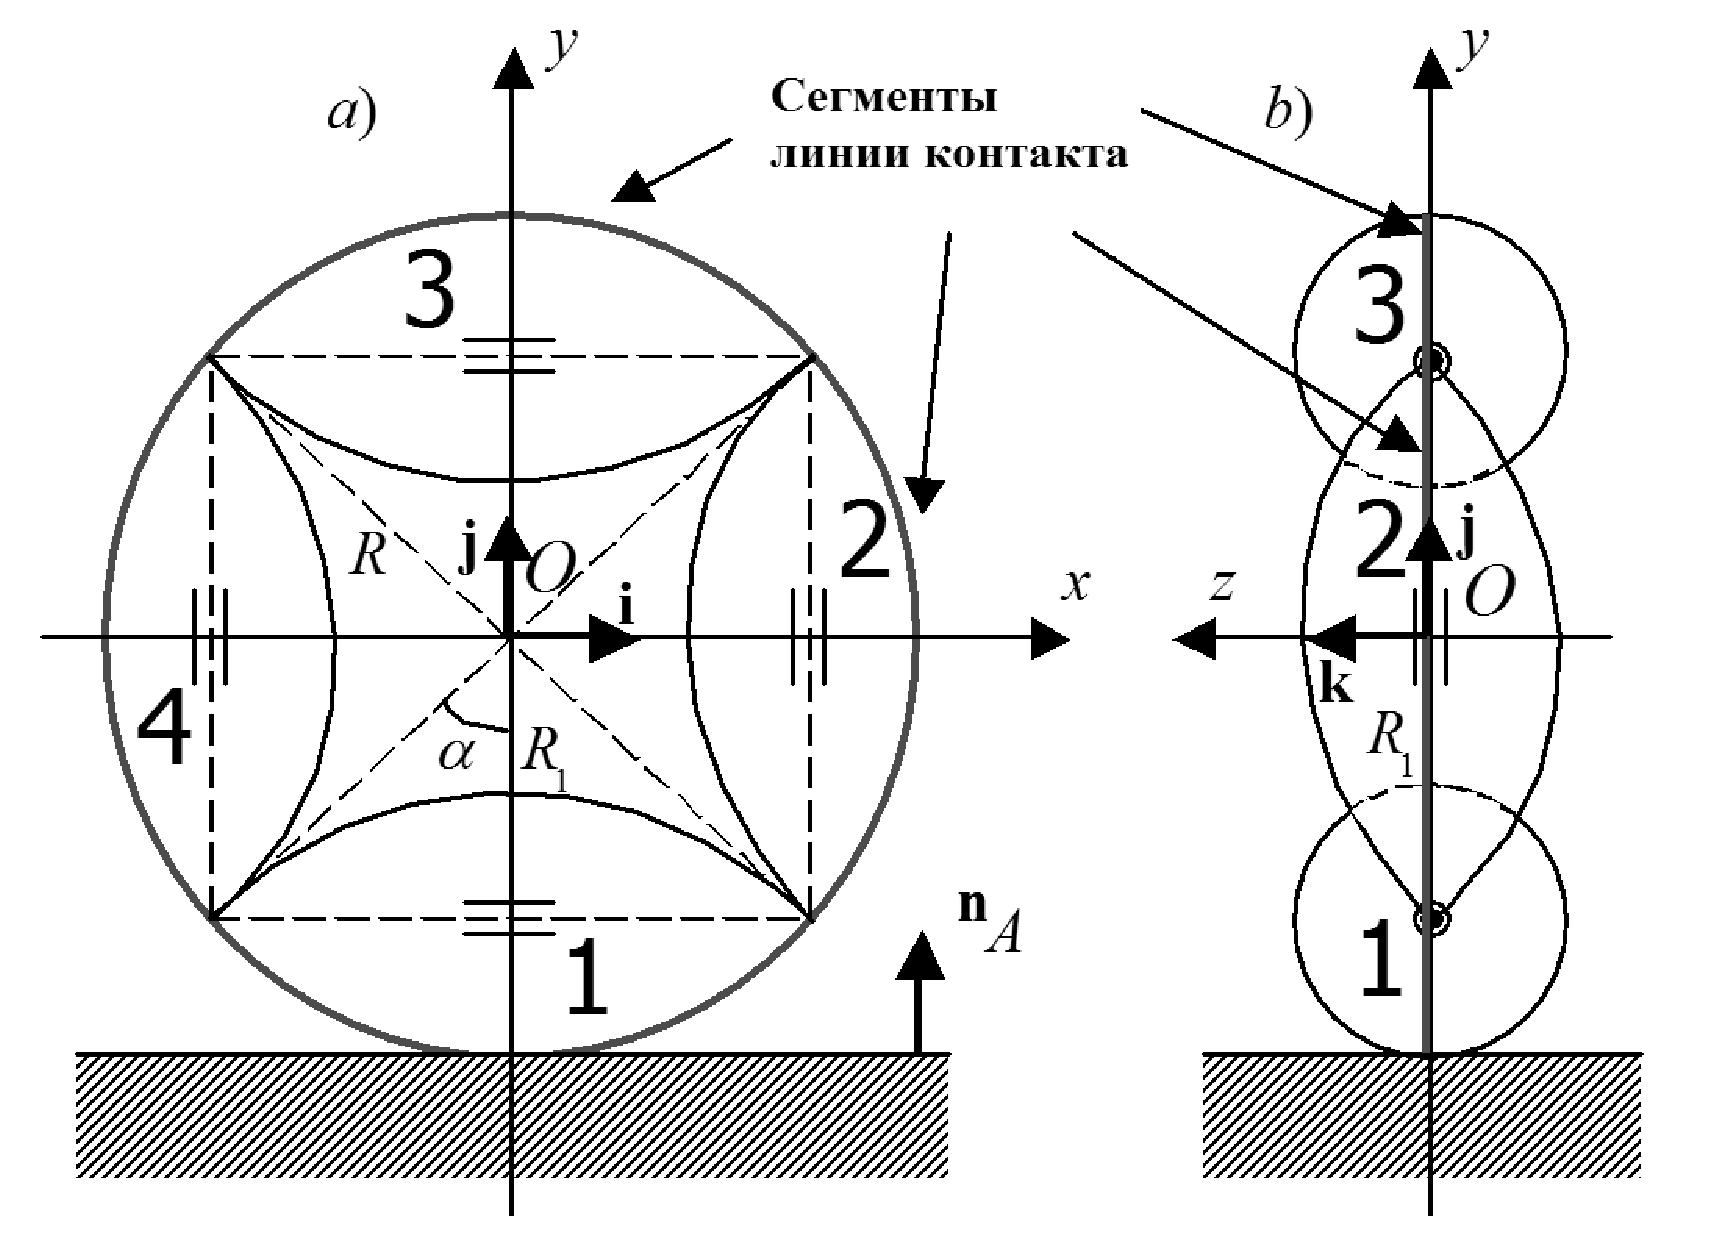
\includegraphics[width=13cm]{content/parts/3_friction/nd/OmniWheel.eps}
\caption{Омни-колесо в вертикальном положении: a) вид сбоку; b) вид спереди.}
\label{OmniWheel}
\end{figure}

Предполагается также, что ролики размещаются на колесе таким образом, что для 
вертикально поставленного омни-колеса проекция линии контактирования наинизшего 
ролика с горизонтальной плоскостью будет состоять из последовательности 
сегментов соответствующих линий контактирования отдельных роликов. Эти сегменты 
сопрягаются таким образом, что при переходе контакта от ролика к ролику 
нормальная составляющая скорости точки ролика, находящейся в точке контакта, к 
горизонтальной плоскости равна нулю. Это означает отсутствие удара по нормали к 
плоскости. В случае коллинеарности осей роликов и плоскости колеса скачки 
скорости скольжения по касательному направлению к горизонтальной плоскости 
также отсутствуют, так как при переходе контакта между роликами их внешние 
поверхности непрерывно вырождаются в точку (в идеализированной модели), что 
означает отсутствие кинематического влияния собственного вращения роликов при 
переходе контакта с ролика на ролик. Так что в результате переключение 
контактов между роликами омни-колеса не приведет к нарушению регулярности 
движения в силу причин ударного характера. Заметим еще раз, что все описанное 
будет справедливо, если колесо все время остается в вертикальном положении.

% На следующем уровне сборки модели несколько колес соединяются с подвижной 
% платформой экипажа при помощи шарнирных связей. В нашем случае количество колес 
% может быть три или более (в зависимости от конструкции экипажа и модели 
% контактирования ролика с полом). На платформе они могут образовывать самые 
% разные конфигурации. В конкретном примере Рис.~\ref{Vehicle} имеется три 
% колеса, образующие равносторонний треугольник в горизонтальной плоскости $zx$. 
% Ось $y$ здесь предполагается вертикальной.

% \begin{figure}[htb]
% \centering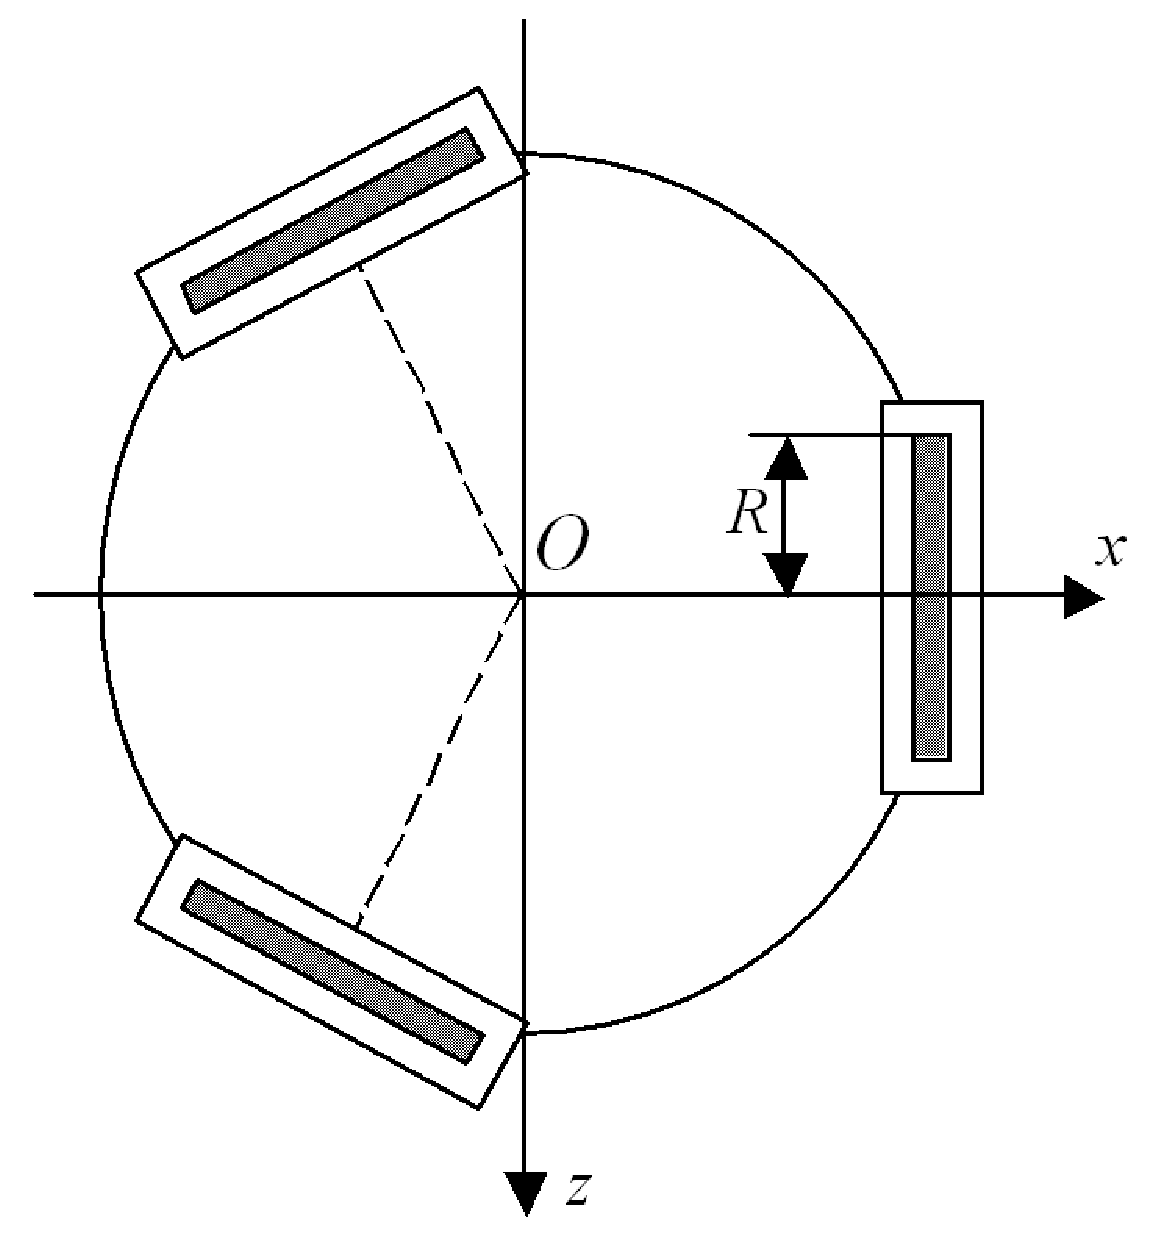
\includegraphics[width=9cm]{content/parts/3_friction/nd/Vehicle.eps}
% \caption{Трехколесный экипаж. Вид сверху.}
% \label{Vehicle}
% \end{figure}

% \section{Модель динамики отдельного ролика.\ }
\label{sec3}
Вначале предположим, что ролик представляет собой осесимметричное 
веретенообразное твердое тело с внешней поверхностью, задаваемой в своих 
собственных осях $Oxyz$ уравнением
\begin{equation}
x^2+\left(\sqrt{y^2+z^2}+R_1\right) ^2=R^2,
\label{3_1}
\end{equation}
где $R$ --- радиус омни-колеса, $R_1=R\cos{\alpha }$ --- расстояние от центра
ролика до центра колеса, $\alpha =\pi /n$ --- половина центрального угла, под
которым ролик виден из центра колеса, $n$ --- количество роликов на колесе.

\begin{figure}[htb]
\centering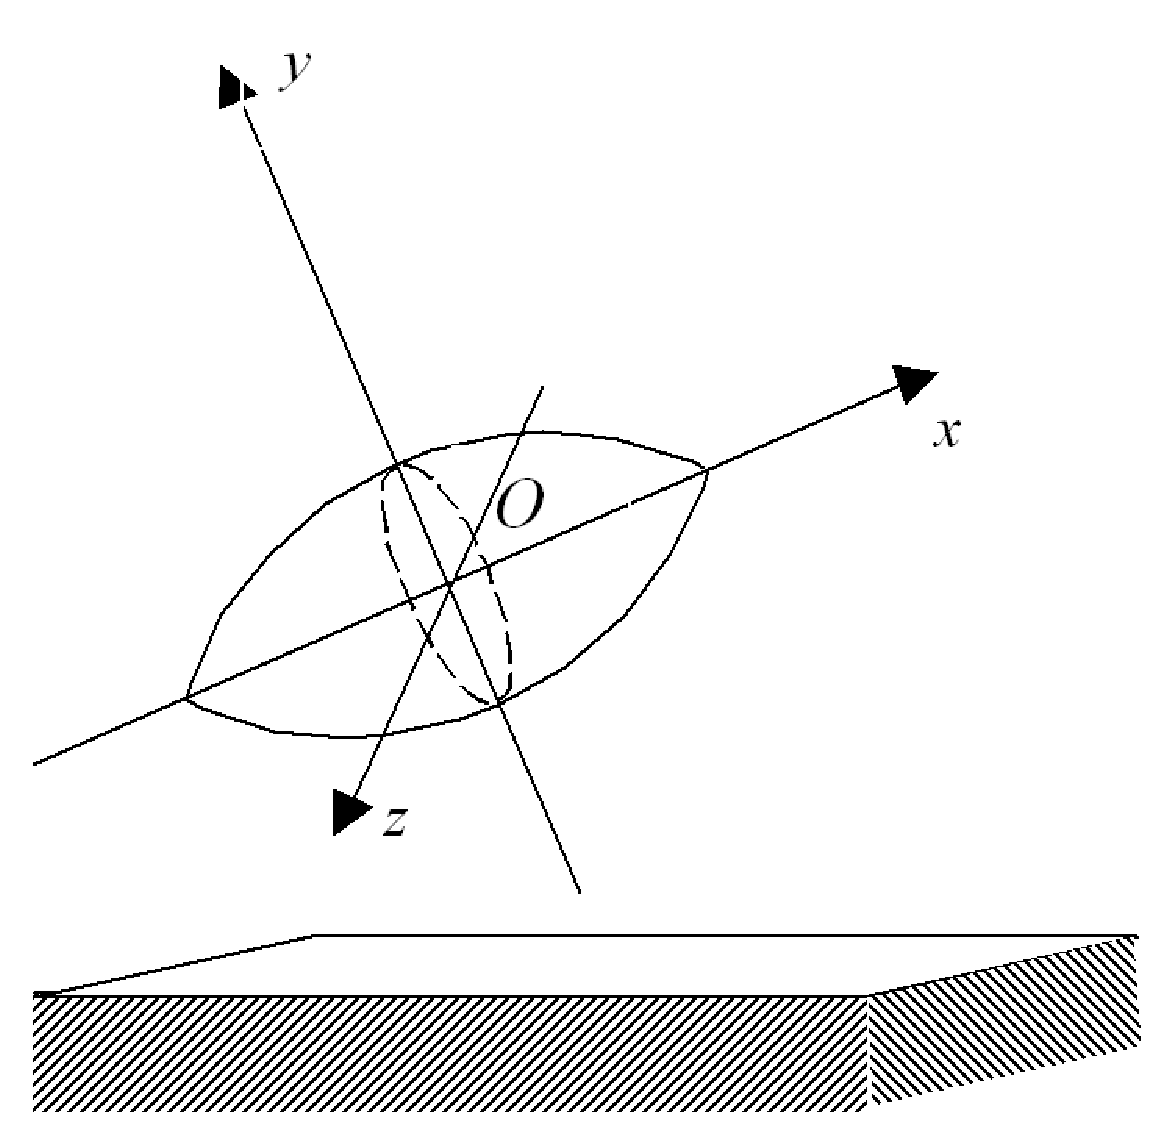
\includegraphics[width=10cm]{content/parts/3_friction/nd/Roller.eps}
\caption{Ролик над горизонтальной плоскостью. Вид сбоку.}
\label{Roller}
\end{figure}

Динамика поступательно-вращательного движения реализуется так, как это описано
в~\cite{Kosenko2007}, в виде уравнений Ньютона -- Эйлера. Причем для 
моделирования вращательного движения твердого тела используется алгебра 
кватернионов~\cite{KosenkoQuaternionRus,Kosenko1998}.

Отдельную проблему представляет задача отслеживания контакта между поверхностью 
ролика и горизонтальной плоскостью. Для моделирования динамики твердого тела с
неудерживающей связью применена технология, описанная в~\cite{Kosenko2006}. В
данном случае можно было бы применить систему алгебраических или 
дифференциально-алгебраических уравнений. Однако эти уравнения вырождаются в 
точках $x=\pm R\sin\alpha $ в координатах ролика. Такое вырождение обычно 
приводит к аварийному завершению вычислительного процесса моделирования.

В нашей задаче положение спасает специфика конфигурации, обеспечивающей 
постоянство вертикального расположения омни-колес. При этом условии можно
указать явную формулу, позволяющую вычислить ближайшую к плоскости точку $P_B$
ролика (Рис.~\ref{ContactScheme}). Этой точке всегда <<противостоит>> её 
вертикальная проекция $P_A$ на плоскость (Рис.~\ref{ContactScheme}).

\begin{figure}[htb]
\centering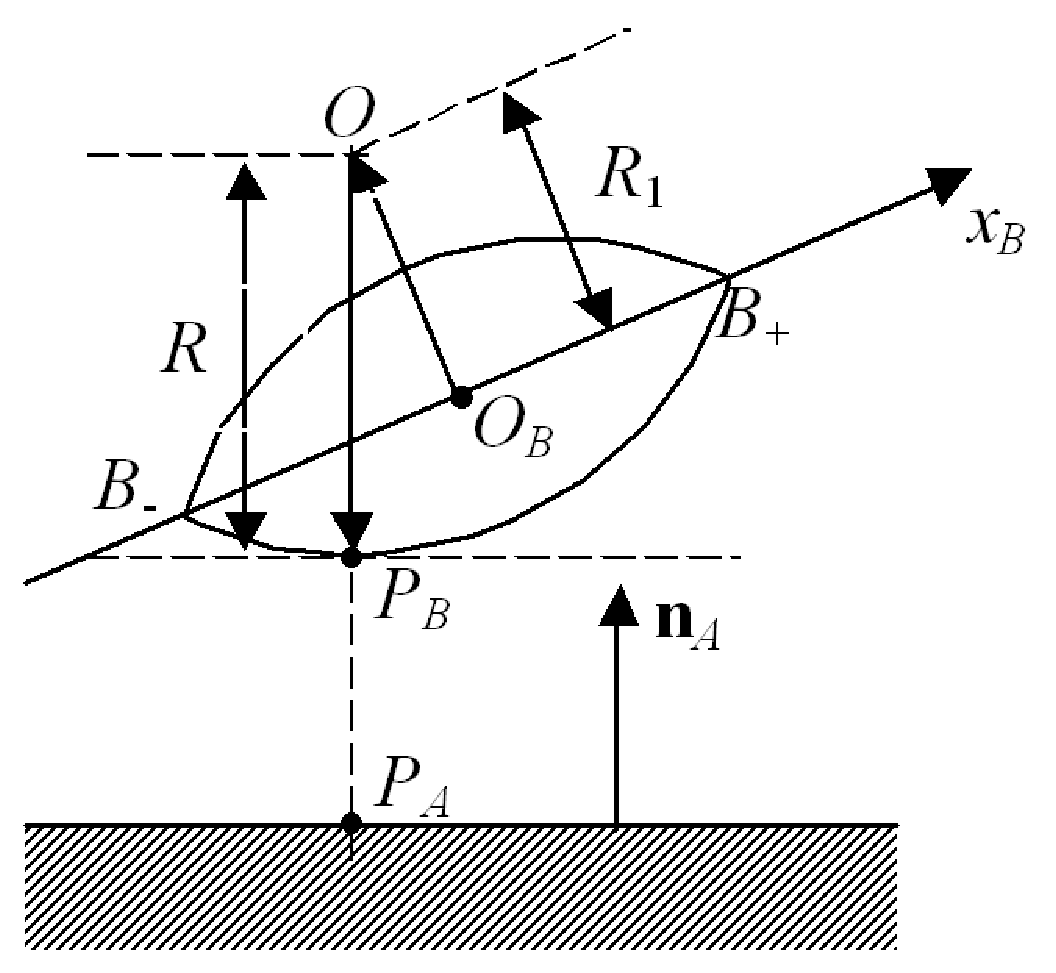
\includegraphics[width=8cm]{content/parts/3_friction/nd/RollerSection.eps}
\caption{Схема отслеживания контакта: вид сбоку отдельного ролика.}
\label{ContactScheme}
\end{figure}

Обозначим символом ${\bf i}_B=(1,0,0)^T$ орт собственной оси ролика $O_Bx_B$.
Этот вектор представлен в системе координат ролика $O_Bx_By_Bz_B$. Пусть $T_B$
--- матрица поворота ролика относительно инерциальной системы координат 
$O_Ax_Ay_Az_A$, связанной с неподвижной плоскостью. Пусть также ${\bf r}_B$ ---
радиус-вектор геометрического центра ролика в текущий момент времени и 
${\bf n}_A=(0,1,0)^T$ --- орт нормали (восходящей вертикали) к плоскости. 
Плоскость условно обозначается нами телом с индексом $A$, ролик --- $B$. Пусть
${\bf d}$ --- горизонтальный орт, вычисляемый по формуле
$$
{\bf d}=\dfrac{T_B{\bf i}_B\times {\bf n}_A}
              {\left| T_B{\bf i}_B\times {\bf n}_A\right|}.
$$
Тогда, очевидно, отрезок $\overrightarrow{O_BO}$, расположенный в вертикальной
плоскости, будет иметь длину $R_1$ и задаваться формулой
$$
\overrightarrow{O_BO}=R_1{\bf d}\times T_B{\bf i}_B.
$$
Здесь $O$ --- центр кривизны окружности вертикального сечения ролика 
(Рис.~\ref{ContactScheme}). Так что самая нижняя точка $P_B$ внешней 
поверхности ролика будет задаваться по формуле
\begin{equation}
{\bf r}_{P_B}={\bf r}_B+R_1{\bf d}\times T_B{\bf i}_B-R{\bf n}_A,
\label{3_2_0}
\end{equation}
поскольку точка $P_B$ лежит на упоминавшейся выше окружности на общей вертикали 
с точкой $O$. Для вычисления положения точки $P_A$ нужно вторую координату 
вектора ${\bf r}_{P_B}$ положить равной нулю
\begin{equation}
{\bf r}_{P_A}=\left( x_{P_B},0,z_{P_B}\right) ^T.
\label{3_2_1}
\end{equation}

Вся описанная выше вычислительная процедура будет справедлива только, если 
вектор $T_B{\bf i}_B$ имеет направление, ограниченное по вертикали углами
$\pm\alpha $. Если соответствующий угол превышает значение $\alpha $, то 
следует положить $P_B=B_{-}$, где $B_{-}$ --- левая концевая точка ролика. Если
же этот угол меньше величины $-\alpha $, нужно положить $P_B=B_{+}$, где 
$B_{+}$ --- правая концевая точка ролика.

В конечном итоге условие контактирования ролика и плоскости можно записать в 
виде
\begin{equation}
\left| T_B{\bf i}_B\cdot {\bf n}_A\right|\le\sin\alpha .
\label{3_2}
\end{equation}
Это условие, однако, позволяет из всего множества роликов колеса выделить 
нижний (контактирующий) и верхний. Чтобы отбросить случай последнего ролика
можно к последнему условию присоединить также требование 
\begin{equation}
y_B<R,
\label{3_3}
\end{equation}
где $y_B$ --- высота центра ролика относительно инерциальной системы координат.

Таким образом, конъюнкция условий (\ref{3_2}) и (\ref{3_3}) означает наличие
контакта. В противном случае, при отсутствии контакта, нормальная реакция 
отсутствует (закон Синьорини). С другой стороны, реализация контакта 
геометрически означает выполнение скалярного условия 
\begin{equation}
y_{P_B}=0,
\label{3_4}
\end{equation}
а его отсутствие --- также скалярного (альтернативного) условия
$$
F_n=0,
$$
где $F_n$ --- нормальная составляющая реакции (в данном случае отсутствующей) 
приложенной в точке $P_B$.

% \begin{figure}[htb]
% \centerline{
% 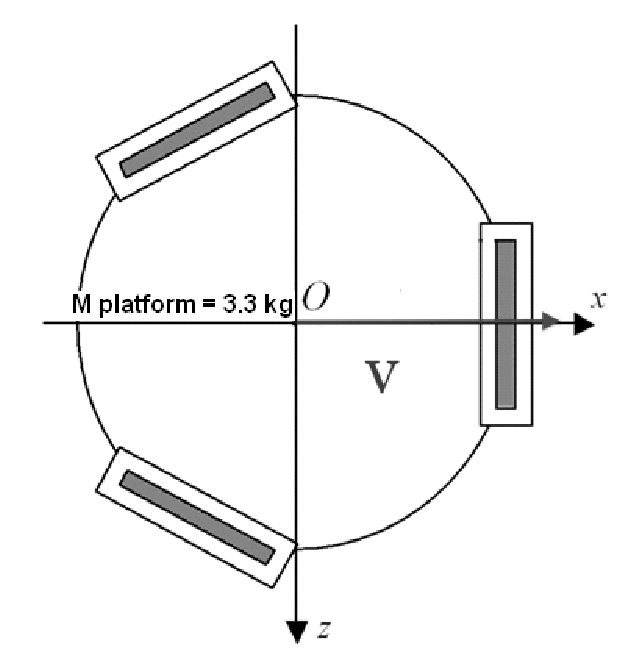
\includegraphics[width=7cm]{content/parts/3_friction/nd/Translat.eps}
% 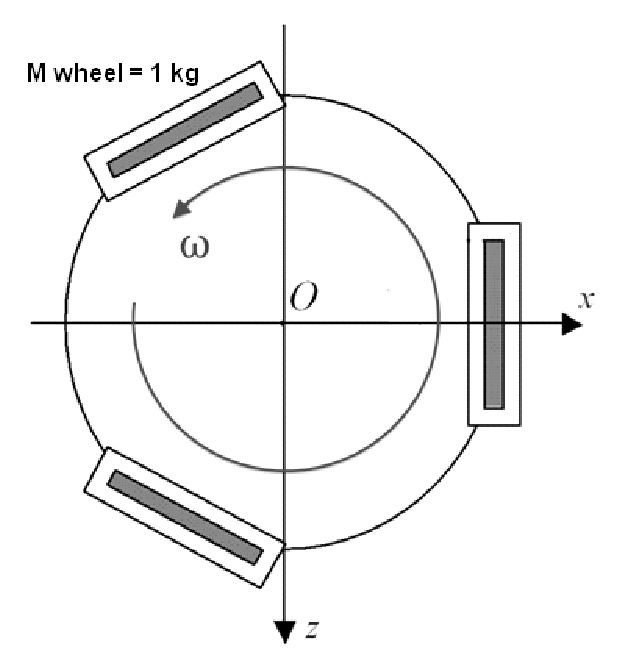
\includegraphics[width=7cm]{content/parts/3_friction/nd/Rotat.eps}
% }
% \caption{Типы движения при верификации модели.}
% \label{TypesOfMotion}
% \end{figure}

Вычислительная практика показала, что уравнения контакта в форме (\ref{3_4})
стабильно приводит к аварийному завершению процесса симуляции динамической 
модели ролика. Аналогичный результат получается, если в качестве уравнения 
контактирования использовать уравнение вида 
$$
v_n=0,
$$
где $v_n$ -- нормальная составляющая скорости точки контактирования, лежащей
на теле $B$, относительно тела $A$ (горизонтальной плоскости). И только 
уравнение вида
$$
\dot{v}_n=0
$$
приводит к требуемому результату -- корректной работе объекта контактирования
(реализованного в данном случае на языке Modelica~\cite{Fritzson}) в процессе 
симуляции модели. Вся реализация процесса контактирования 
выполнена в предположении точечного <<твердого>> контакта твердых тел без 
какой-либо податливости.

Колеса, собранные в экипаж, с неизбежностью будут сохранять вертикальное 
положение. Поэтому упрощенный алгоритм отслеживания контакта, описанный выше,
всегда будет работать правильно.

% \section{Отслеживание контакта в случае \textit{mecanum} колеса}

Обозначим угол наклона оси ролика к плоскости колеса $\psi$. В предыдущей конфигурации этот угол равен нулю. Расширим алгоритм отслеживания контакта, описанный выше для случая $\psi = 0$ на конфигурацию \textit{mecanum}, $\psi > 0$. В этом случае, в первую очередь, отметим отличия в геометрической форме роликов. Каждый ролик -- это твердое тело, ограниченное поверхностью вращения некоторой кривой вокруг его оси. В случае $\psi = 0$ эта кривая -- дуга окружности, но при $\psi > 0$, для того, чтобы проекция внежней границы колеса на его плоскость оставалась окружностью, форма роликов должна быть более сложной -- образующая кривая становится алгебраической кривой четвертого порядка \cite{Gfrerrer2008}.

\begin{figure}[H]
    \centering
    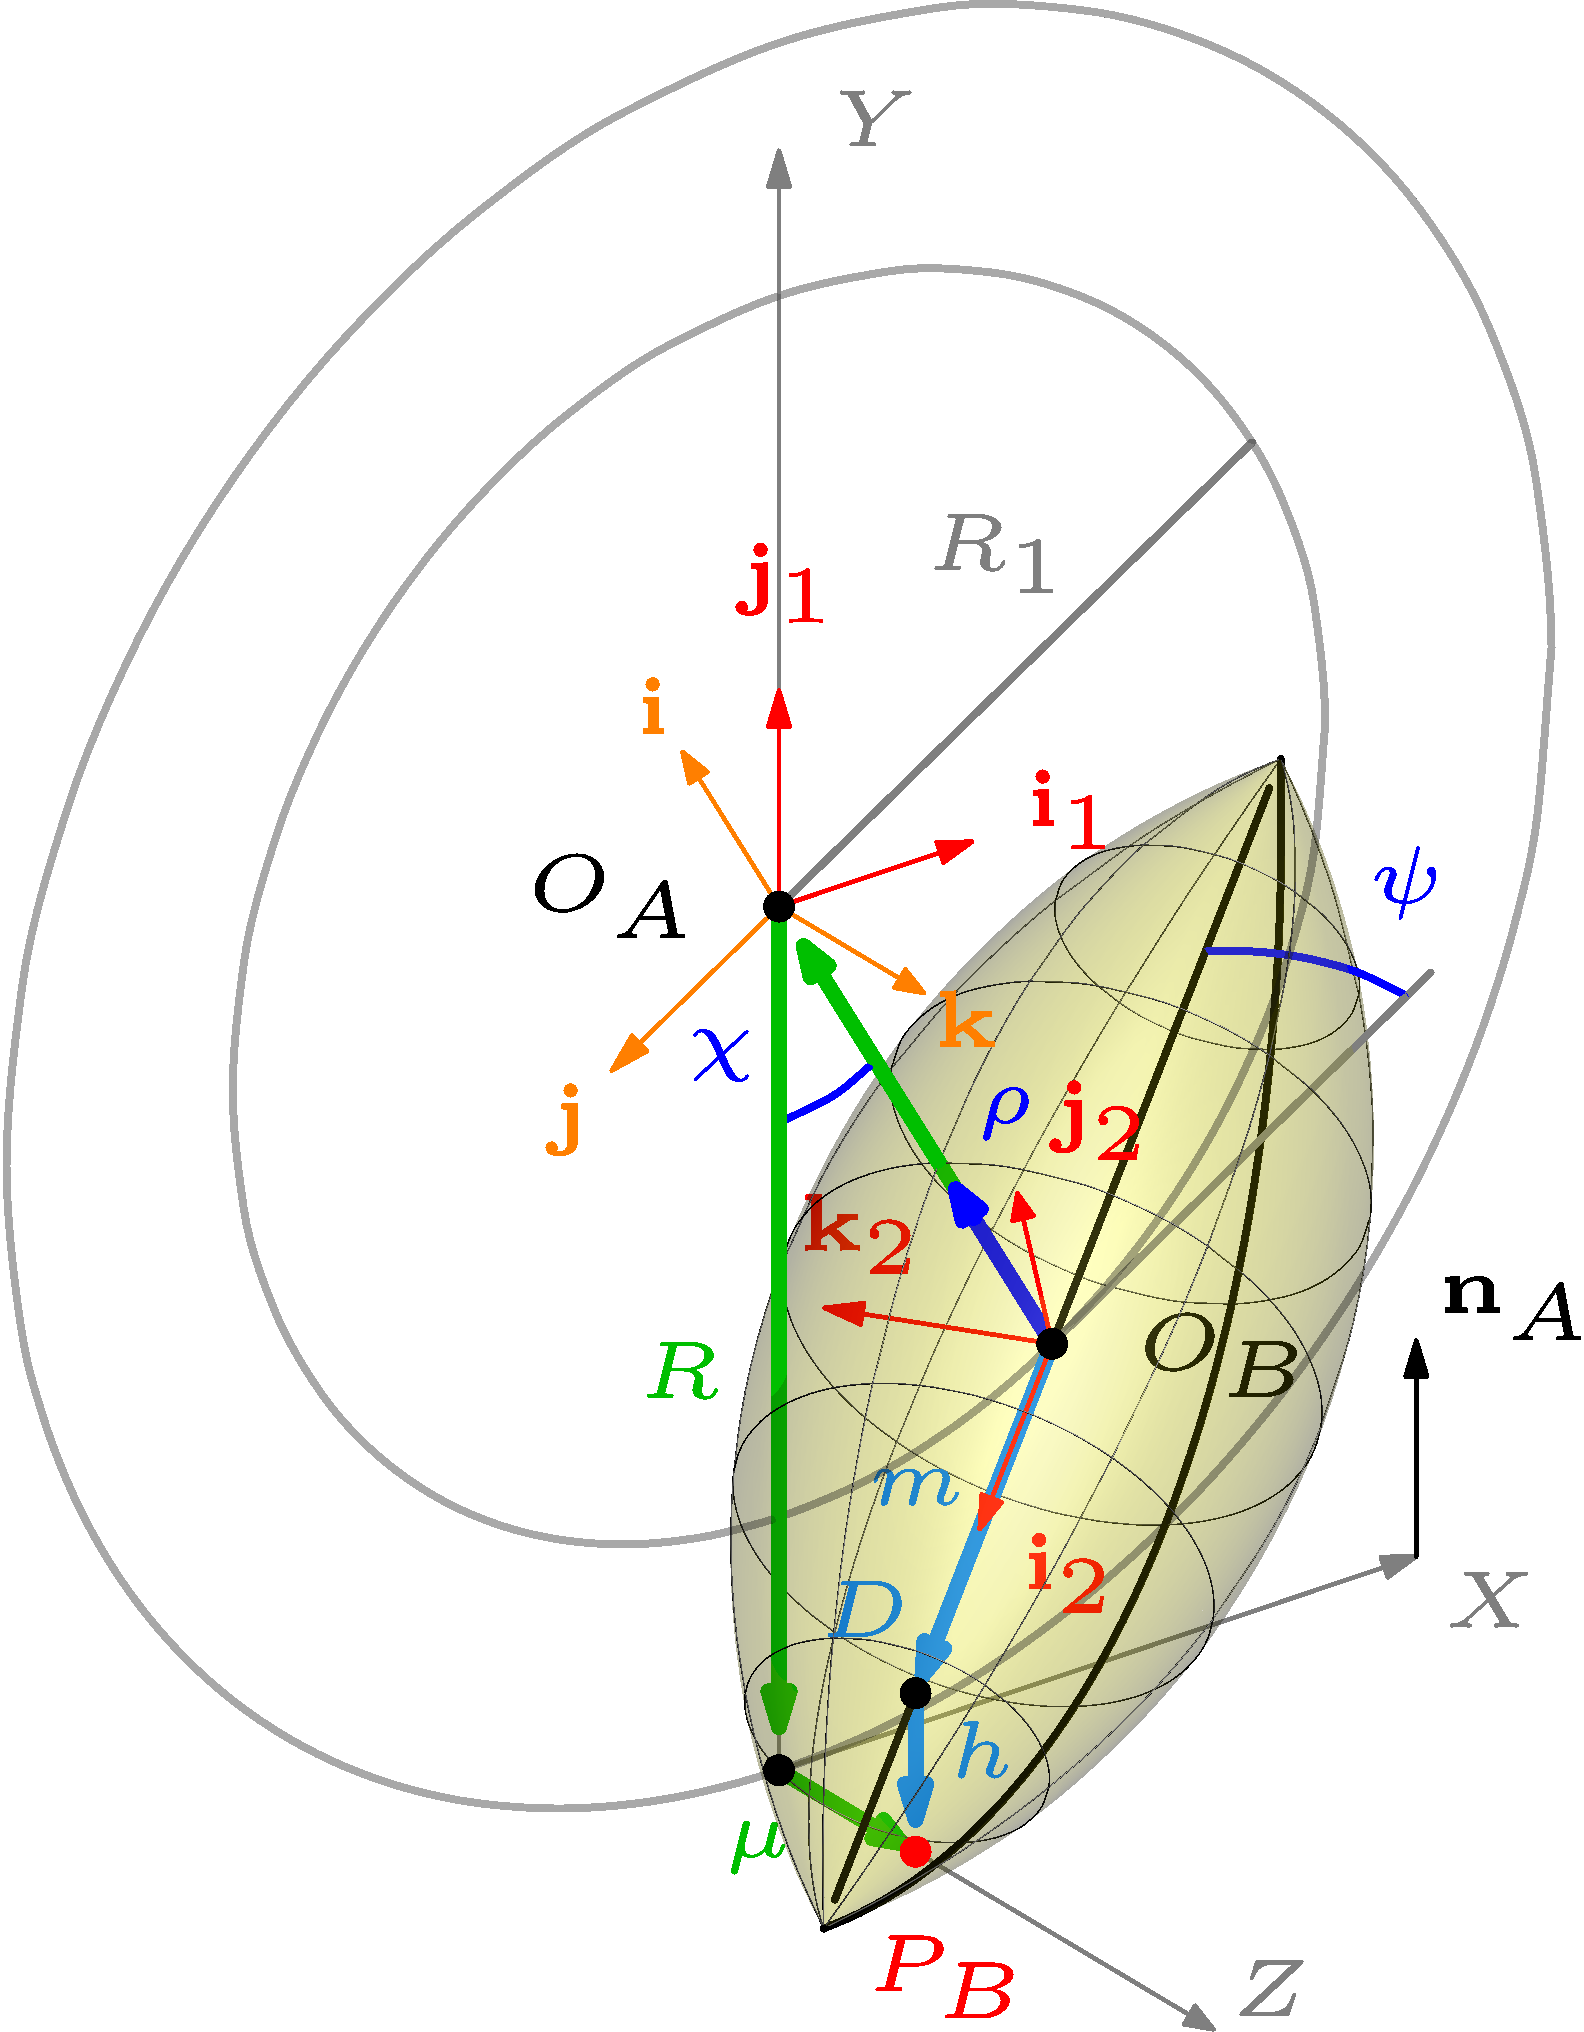
\includegraphics[width=0.5\textwidth]{./content/pic/asy/pic_mecanum.png}
    \caption{Отслеживание контакта для колеса \textit{mecanum}}
    \label{fig:mecanum}
\end{figure}

\textbf{Неявный алгоритм отслеживания контакта}

Здесь, как и всюду, будем предполагать, что плоскость колеса вертикальна во все время движения.

Введем систему отсчета $O_A{\bf i}{\bf j}{\bf k}$, жестко связанную с колесом (см. фиг.~\ref{fig:mecanum}), с началом в его центре $O_A$. Вектор ${\bf k}$ направлен вдоль оси колеса, ${\bf i}$ и ${\bf j}$ лежат в его плоскости.

Введем также две вспомогательные системы отсчета $O_A{\bf i}_1{\bf j}_1{\bf k}_1$ и $O_B{\bf i}_2{\bf j}_2{\bf k}_2$, где $O_B$ -- центр ролика.

Вектор ${\bf i}_2$ направим вдоль оси симметрии ролика, см. фиг.~\ref{ContactScheme}.
Вектор ${\bf j}_2$ ортогонален ${\bf i}_2$ и лежит в вертикальной плоскости.
Третий вектор ${\bf k}_2$ определяется естественным образом как
$$
{\bf k}_2={\bf i}_2\times {\bf j}_2.
$$
% \begin{figure}[hb]
% \centerline{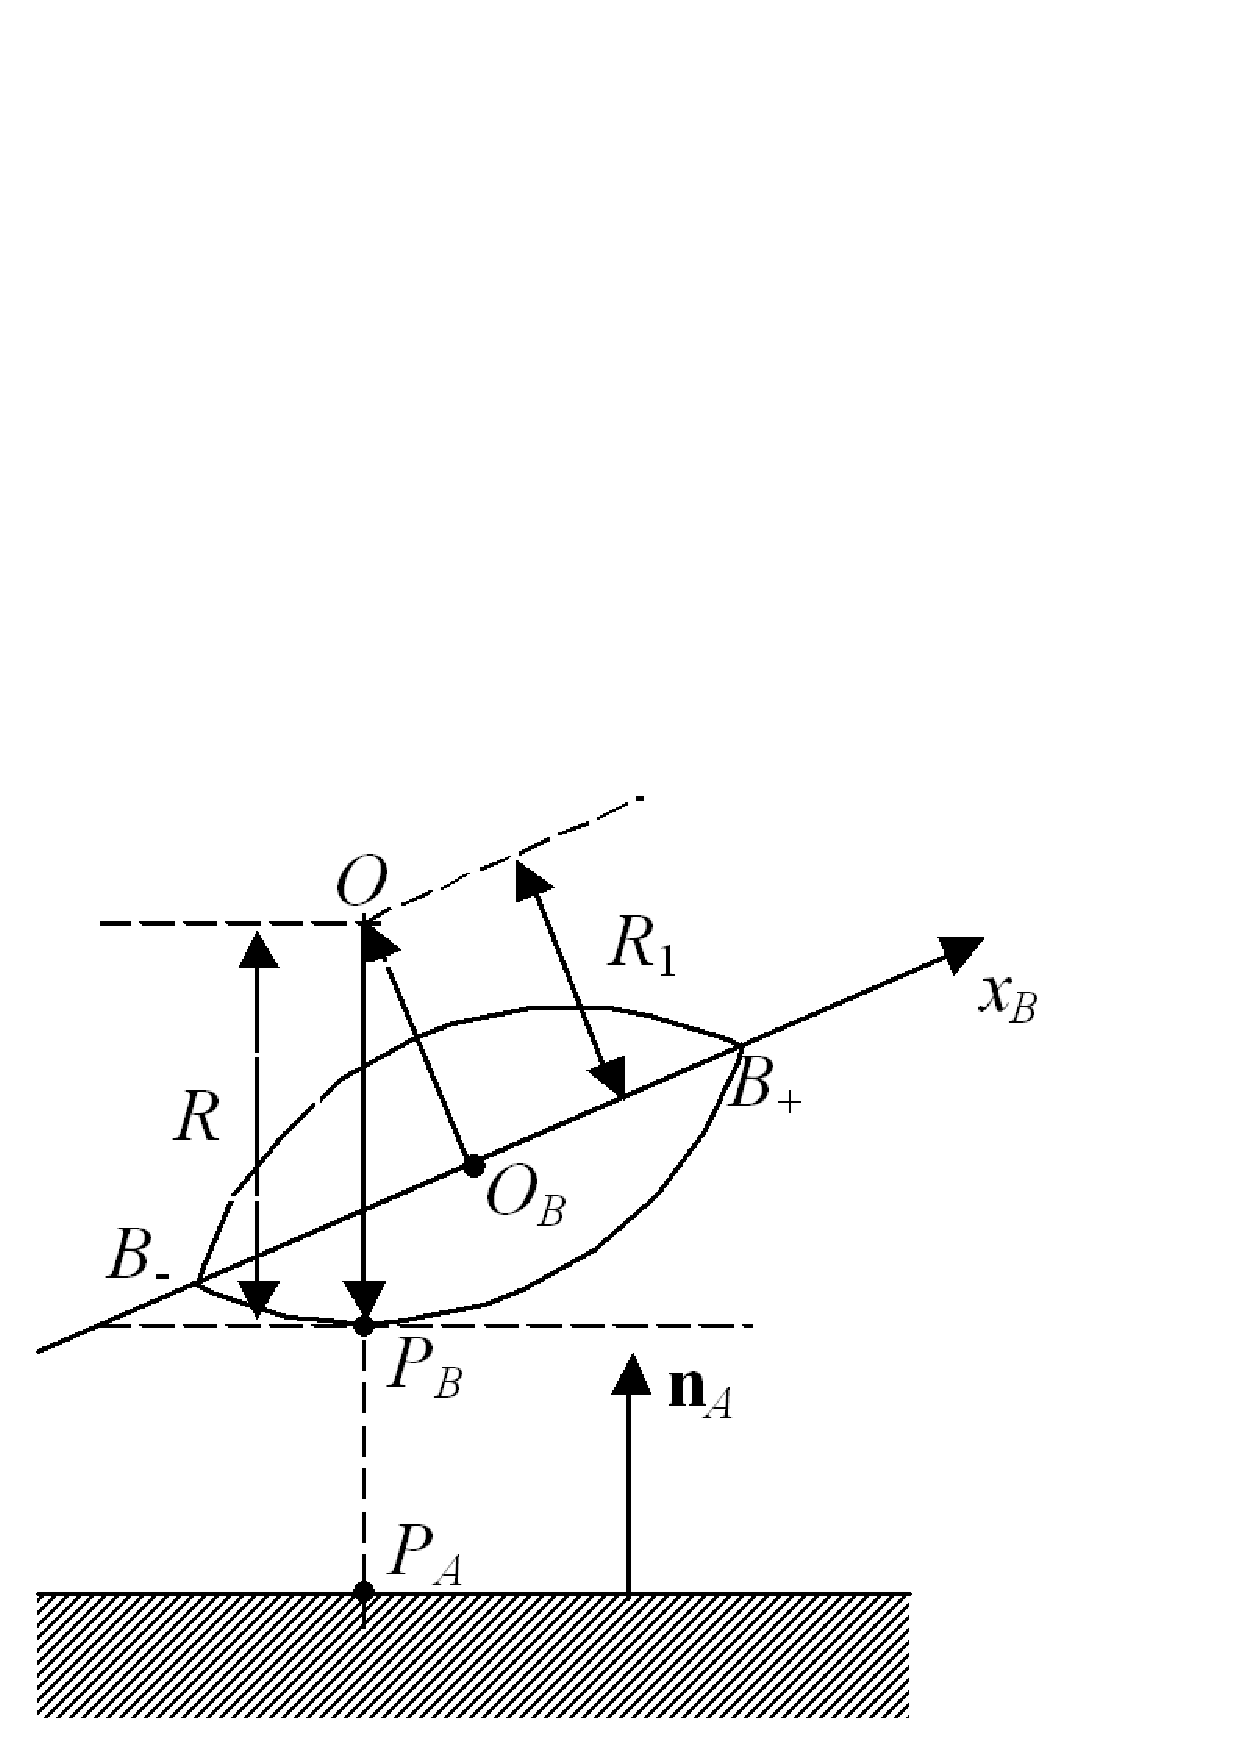
\includegraphics[bb= 0cm 0cm 20cm 17cm,scale=0.30]{RollerSection.png}}
% \caption{Contact tracking scheme.}
% \label{ContactScheme}
% \end{figure}

Во время счета компоненты всех векторов задаются относительно неподвижной системы отсчета, а положения и ориентации всех тел системы в момент времени $t\in [t_0,t_1]$ считаются известными.

Таким образом, для системы $O_B{\bf i}_2{\bf j}_2{\bf k}_2$, имеем:
$$
{\bf i}_2=T_B\cdot (1,0,0)^T,\quad\vecrho =
\left( {\bf r}_{O_A}-{\bf r}_{O_B}\right) /
\left| {\bf r}_{O_A}-{\bf r}_{O_B}\right| ,
$$
где $T_B$ -- матрица ориентации ролика, а единичный вектор $\vecrho$ направлен вдоль луча, выпущенного из центра колеса $O_A$ в сторону центра ролика $O_B$.

Вектор ${\bf i}_1$ лежит на пересечении плоскости колеса и горизонтальной плоскости.
${\bf k}_1 = {\bf k}$ ортогонален плоскости колеса и совпадает с одним из векторов базиса, связанного с колесом, и всегда горизонтален.
Тогда имеем ${\bf j}_1(t)=(0,1,0)^T$ и ${\bf i}_1(t)={\bf j}_1(t)\times {\bf k}_1(t)$.

Теперь рассмотрим соотношения, позволяющие вычислить компоненты базисных векторов векторов системы отсчета $O_B{\bf i}_2{\bf j}_2{\bf k}_2$.

Отметим, что вектор ${\bf i}_2$, направленный вдоль оси ролика, по определению не может принять вертикальное положение, если ролик находится в контакте с опорной плоскостью.
Более того, в случае \textit{mecanum} ролик повернут на постоянный угол $\psi > 0$ относительно оси $O_AO_B$, и потому во все время движения верно соотношение ${\bf i}_2\ne (0,1,0)^T$.
Таким образом, вектор ${\bf c}={\bf i}_2\times (0,1,0)^T$ также отличен от нуля.
Положим ${\bf k}_2={\bf c}/|{\bf c}|$. Теперь можно определить ${\bf j}_2$ как
${\bf j}_2={\bf k}_2\times {\bf i}_2$.

Для определения компонент вектора $\vecrho$ воспользуемся кинематическими соотношениями, условиями ортогональности векторов, следующими из определений введенных систем отсчета:
$$
\vecrho\cdot {\bf i}_2=0,\quad\vecrho\cdot {\bf k}_1=0.
$$
и их дифференциальными вариантами:
$$
\dfrac{d}{dt}\vecrho\cdot {\bf i}_2+\vecrho\cdot\dfrac{d}{dt}{\bf i}_2=0,\quad
\dfrac{d}{dt}\vecrho\cdot {\bf k}_1+\vecrho\cdot\dfrac{d}{dt}{\bf k}_1=0.
$$

Величина $c_{\beta }=\cos\beta ={\bf i}_2\cdot (0,1,0)^T$ косинуса угла $\beta $ наклона оси ролика к вертикали $(0,1,0)^T$ также играет важную роль в алгоритме отслеживания контакта.

Если текущее значение переменной величины $c_{\beta }$ меньше некоторого уровня $c_{\beta\max }$, и если одновременно расстояние от центра ролика $O_B$ до опорной плоскости меньше радиуса колеса $R$, то ролик находится в контакте с опорной плоскостью. В противном случае контакт отсутствует.

% Remark here that usually to arrange the unilateral constraint in the multibody
% system dynamics model the developer has to implement anything like hybrid 
% automata construct. In our omni wheel model on the contrary this is not the 
% case. It turned out sufficient to implement ``simple'' ``{\tt if}'' construct 
% to switch states ``contact'' and ``no contact'' for each individual roller, and
% simultaneously to advance forward ``contact'' state from one roller to its 
% neighbour. The whole picture looks like from time to time neighbouring rollers
% mutually exchange by their states.

На фиг.~\ref{ContactScheme} также легко видеть, что координаты точки $P_B$ контакта ролика и плоскости даются выражением
$$
{\bf r}_{P_B}={\bf r}_{O_B}+R_1\vecrho -R{\bf j}_1+\mu {\bf k}_1,
$$
где число $\mu$ требуется вычислить (см. фиг.~\ref{fig:mecanum}). Здесь величина $R_1$ равна расстоянию между точками $O_A$ и $O_B$.
Чтобы получить число $\mu$, умножим последнее уравнение скалярно на ${\bf k}_2$. Отсюда
$$
\mu =\left[R{\bf j}_1\cdot{\bf k}_2-R_1{\vecrho }\cdot {\bf k}_2\right] /
{\bf k}_1\cdot{\bf k}_2,
$$
поскольку ${\bf r}_{P_B}-{\bf r}_{O_B}$ лежит в вертикальном сечении осесимметричной поверхности ролика, и вектор ${\bf k}_2$ по построению ортогонален этому сечению. В результате радиус-вектор ${\bf r}_{P_B}$ точки контакта $P_B$ определяется однозначно.

\textbf{Явный алгоритм отслеживания контакта}

Еще одним способом вычисления компонент радиус-вектора ${\bf r}_{P_B}$ точки контакта point $P_B$ или, точнее, точки ролика, ближайшей к опорной плоскости, является применение следующего набора равенств (см. фиг.~\ref{fig:mecanum}):
% Лучше всего этот способ иллюстрирует геометрическая схема на фиг.~\ref{fig:figure3}.
% STEPANOV
% Во-первых, имеем
% $$
% {\bf r}_{P_B}={\bf r}_{O_B}+\overrightarrow{CD}+\overrightarrow{DG},\quad
% \overrightarrow{CD}=-m{\bf i}_2,\quad\overrightarrow{DG}=-h{\bf j}_1,
% $$
$$
{\bf r}_{P_B}={\bf r}_{O_B}+\overrightarrow{O_BD}+\overrightarrow{DP_B},\quad
\overrightarrow{O_BD}=-m{\bf i}_2,\quad\overrightarrow{DP_B}=-h{\bf j}_1,
$$
% STEPANOV
% где $m=R_1\sin q / \cos q/\cos\psi $, $h=R-R_1/\cos q$. 
% Здесь $q$ -- текущее значение угла отклонения вектора ${\bf r}_{O_A}-{\bf r}_{O_B}$ от 
где $m=R_1\sin\chi / \cos\chi/\cos\psi $, $h=R-R_1/\cos\chi$. Здесь $\chi$ -- текущее значение угла отклонения вектора ${\bf r}_{O_A}-{\bf r}_{O_B}$ от 
вертикали. Таким образом,
$$
\cos\chi=\vecrho\cdot{\bf n}_A, \quad \sin\chi=
\left({\bf n}_A\times\vecrho\right)\cdot {\bf k}_1.
$$
% STEPANOV
% $$
% \cos q=\vecrho\cdot{\bf n}_A,\quad\sin q=
% \left({\bf n}_A\times\vecrho\right)\cdot {\bf k}_1.
% $$
\begin{figure*}[H]
\centerline{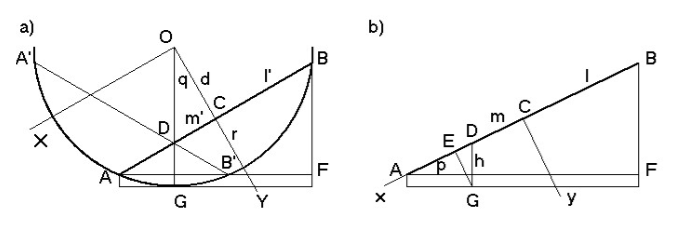
\includegraphics[scale=0.7]{content/parts/3_friction/mo2015/stepanov.png}}
\caption{Явная схема отслеживания контакта}
\label{fig:figure3}
\end{figure*}
% STEPANOV
% Поясним фиг.~\ref{fig:figure3} более детально.
% В части (а) приведена проекция колеса на его плоскость и соответственно, проекция ролика, находящегося в общем положении так, что его ось находится под углом к плоскости проекции.
% Далее, $G$ -- точка контакта между роликом и опорной горизонтальной плоскостью в настоящий момент, $m'$ -- отрезок $DC$ проекции оси ролика на плоскость колеса. Легко видеть, что длина этой проекции равна $m'=m\cos\psi$, поскольку ось ролика $AB$ повернута вокруг прямой $OC$ на угол $\psi$, см. вертикальное сечение, содержащее ось ролика в части (b).
% Таким образом, чтобу получить точку контакта $P_B$ ($G$ на рис.), нужно пройти два отрезка прямых от центра ролика $O_B$ ($C$ на рис.): (a)~отрезок $CD$ оси ролика длины $m$; 
% (b)~отрезок $DG$ вертикали длины $h$.
% Как было отмечено выше, все величины требуется явно выразить через известные координаты.
Кривая, образующая поверхность ролика, пересекает его ось в окрестности острия и переходит на противоположную сторону (параметризация образующей кривой, поверхности ролика и сечения этой поверхности плоскостью, содержащей ось ролика, приведены в \cite{Gfrerrer2008}), в связи с чем
% Чтобы исключить <<перекрытие>> роликов, т.е. ситуацию, при которой два ролика могут находиться в контакте одновременно, более чем при одном (граничном) значении угла поворота колеса,
необходимо ограничить длины роликов величиной
$$
L=2R\sin\alpha / \cos\psi,
$$
где $\alpha$ -- половина угла раствора дуги окружности, ограничивающей проекцию ролика на плоскость колеса.
При такой конструкции переход колеса с одного ролика на другой происходит мгновенно.
% и при этом их концы оказываются усечены.
% Подробно форма кривой, образующей поверхность роликов, описана в \cite{Gfrerrer2008}.
Отметим, что при этом след колеса на плоскости имеет разрыв, поскольку точка контакта мгновенно переходит на противоположный <<борт>> колеса. Это обстоятельство, впрочем, не препятствует эффективному численному решению.

Описанные алгоритмы отслеживания контакта дают практически одинаковые результаты, относительные различия между которыми имеют порядок $10^{-8}$. Предсказуемо, явный алгоритм быстрее приблизительно в $1.5$ раза.

% \section{Моделирование трения в контакте}

Конструкция омни-колеса такова, что в каждый момент времени имеется имеется только один ролик, контактирующий с опорной поверхностью. Для остальных роликов при этом во время расчета алгоритм отслеживания контакта продолжает работать, генерируя нулевые реакции.

В случае фактического выполнения контакта помимо нормальной реакции вычисляется также её касательная составляющая, сила трения. Для касательного контактного усилия имеется множество различных моделей. Мы остановились на реализации двух случаев при одноточечном твердотельном контакте:
\begin{enumerate}
    \item {
        регуляризованное сухое трение
        $$
            \vec{F}_{\text{тр}} = -\mu N \vec{v}_{C}
                \left\{
                    \begin{array}{ll}
                        \ddfrac{1}{\delta}, \enspace |\vec{v}_{C}| < \delta \ll 1 \vspace{7pt}\\
                        \ddfrac{1}{|\vec{v}_{C}|}\enspace \text{иначе}
                    \end{array}
                \right.
        $$
    }
    \item {
        вязкое трение
        $$
            \vec{F}_{\text{тр}} = -\gamma\vec{v}_{C}
        $$
    }
\end{enumerate}

Как известно, идеальный <<сухой>> случай реализовать не удается из-за разрыва в правой части уравнений движения, поэтому вместо разрывной функции от касательной скорости относительного скольжения контактирующих поверхностей, в первом случае используется её регуляризованный в нуле вариант. Вместо функции $\mathrm{sign}$ применяется функция насыщения, представляющая собой линейный участок с достаточно большим угловым коэффициентом в окрестности нуля. Для таких функций известен результат~\cite{Novozhilov1991} о близости аппроксимирующего движения и движения, соответствующего точному случаю разрывной функции $\mathrm{sign}$. В целом, реализация модели неудерживающей связи основана на результатах~\cite{Kosenko2006unilat}.

\section{Верификация}
% \subsection{Гипотеза о близости решений}
В литературе представлены \cite{Borisov2011, formalskii, ZobovaTatarinovPMM} работы, рассматривающие омниколеса в предположении, что массой и инерцией роликов можно пренебречь, налагающие на систему неголономные связи, ограничивающие направление скорости скольжения в точках контакта колес с поверхностью, на которой стоит экипаж, и не вводящие силу трения в контакте, т.е. считающие скольжение идеальным. Эти идеализированные модели имеют существенно меньше степеней свободы, чем "реальный" омниэкипаж, и легче поддаются аналитическому исследованию.\\

Описанные модели можно использовать для верификации построенной физически-ориентированной модели, рассматривая некоторые элементарные виды движений. Максимальное соответствие построенной модели упомянутым неголономным может быть достигнуто при уменьшении вляиния массы роликов на динамику колеса, а именно, при уменьшении их массы с сохранением общей массы колеса с роликами. На этом предположении и основан наш подход к верификации.\\

\subsection{Проверочная модель}

Для верификации использованы результаты работы \cite{Borisov2011} как новейшей из неголономных моделей динамики свободной тележки с омниколесами на плоскости.\\

Авторы \cite{Borisov2011} принимают простейшую модель омниколеса как плоского диска, для которого скорость точки контакта с опорной поверхностью направлена вдоль прямой, составляющей некоторый угол $\delta$ с плоскостью колеса (см. рис.~\ref{fig:bor_wheel_scheme}). Связь, наложенная на колесо в таком случае имеет вид
$$\vec{v_Q}\cdot\vec{\alpha} = 0,$$
где $\vec{v_Q}$ - скорость точки контакта, $\vec{\alpha}$ - единичный вектор вдоль оси закрепления роликов.\\

\begin{figure}[ht!]
    \centering
    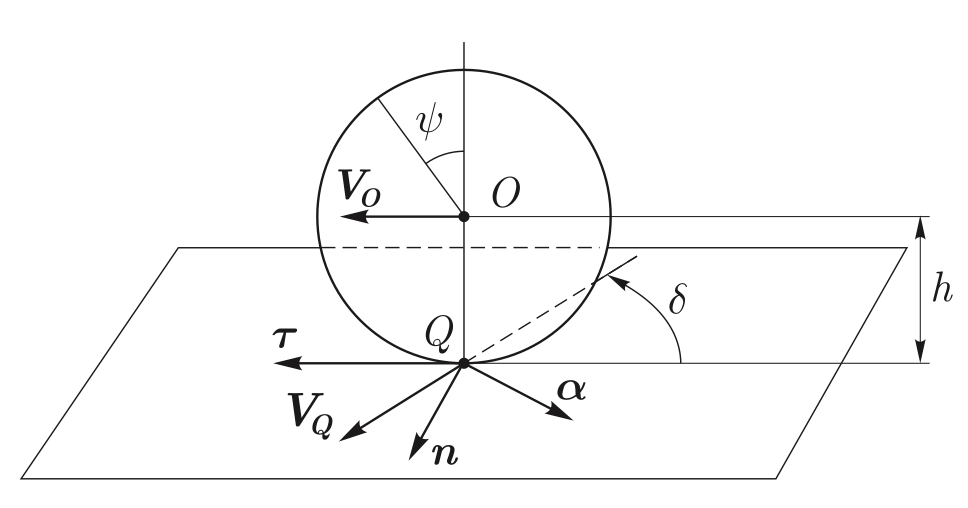
\includegraphics[width=0.75\textwidth]{content/parts/3_friction/diploma/img/art/bor_wheel_scheme.png}
    \caption{Неголономная модель колеса}
    \label{fig:bor_wheel_scheme}
\end{figure}

Авторы \cite{Borisov2011} получают уравнения движения для экипажа с произвольным количеством колес, закрепленных так, что их оси неподвижны относительно платформы, а оси роликов повернуты на произвольные углы относительно плоскостей соответствующих колес (см.рис.~\ref{fig:bor_vehicle}).

\begin{figure}[ht!]
    \centering
    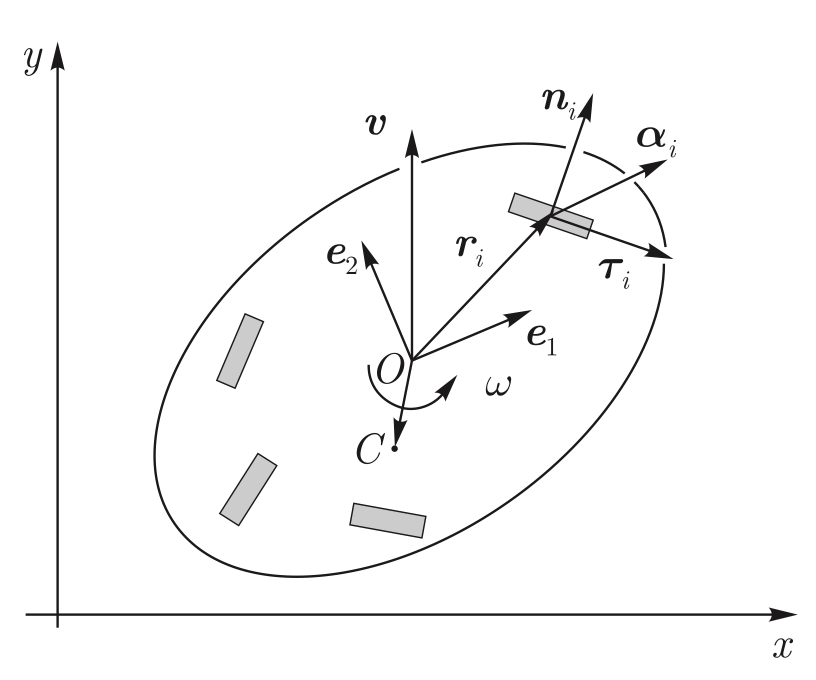
\includegraphics[width=0.75\textwidth]{content/parts/3_friction/diploma/img/art/bor_vehicle.png}
    \caption{Неголономная модель экипажа}
    \label{fig:bor_vehicle}
\end{figure}

Вводится подвижная система отсчета, связанная с платформой экипажа (см.рис.~\ref{fig:bor_vehicle}). Уравнения свободного движения имеют вид:
\begin{eqnarray*}
(\Gamma+mE)\dot{\vec{v}} + m\dot{\omega}(J\vec{r_C}+R)+m\omega J(\vec{v} + \omega J\vec{r_C}) = 0,\\
\hat{I}\dot{\omega} + m(J\vec{r_C}+\vec{r})\cdot\dot{\vec{v}}+m\omega\vec{v}\cdot\vec{r_C} = 0,\\
\dot{x} = v_1\cos\phi - v_2\sin\phi, \dot{x} = v_1\sin\phi + v_2\cos\phi, \dot{\phi} = \omega,\\
\Gamma_{kl} = \sum_i \frac{I_i}{s_i^2 h_i^2}\alpha_i^k\alpha_i^l, R = m^{-1}\sum_i \frac{I_i}{s_i^2 h_i^2}(J\vec{r_i}\cdot \alpha_i) \alpha_i,\\
\hat{I} = I + \sum_i \frac{I_i}{s_i^2 h_i}(J\vec{r_i}\cdot \alpha_i)^2,
\end{eqnarray*}%
\newline
где $\hat{I}$ - суммарный момент инерции системы относительно вертикальной оси, проходящей через начало $O$ подвижной системы отсчета,\newline
$I$ - момент инерции платформы относительно той же прямой,\newline
$I_i$ - моменты инерции колес относительно их диаметров,\newline
$s_i = \sin\delta_i$, $h_i$ - радиусы колес,\newline
$\vec{r_i}$ - точки закрепления осей колес в подвижной системе,\newline
$J = \left(\begin{array}{cc}0 & 1\\-1 & 0\end{array}\right)$,\newline
$x,y,\phi$ - координаты точки $O$ и угол поворота платформы экипажа вокруг вертикальной оси,\newline
$\vec{v}, \omega$ - вектор скорости точки $O$ и скорость поворота платформы,\newline
$\vec{r_C}$ - координаты центра масс экипажа в подвижных осях,
$E$ - единичная матрица.\\

% Данная неголономная модель экипажа также реализована на языке Modelica \cite{ModelicaSpec} как часть упомянутой библиотеки \cite{KosenkoBond}. Таким образом, возможно проведение сравнительного анализа физически-ориентированной и идеализированной моделей и верифкация.


\subsection{Два типа движений}
Задавая параметры экипажа, такие как массы его частей, их моменты инерции, геометрические размеры, положения, а также начальные данные - скорость центра масс и угловую скорость платформы, - и выполняя согласованные расчеты для двух реализаций - физической и идеальной - можно получить достаточно близкие движения при достаточно малой доле массы роликов.\\

\begin{figure}[!ht]
    \centering
    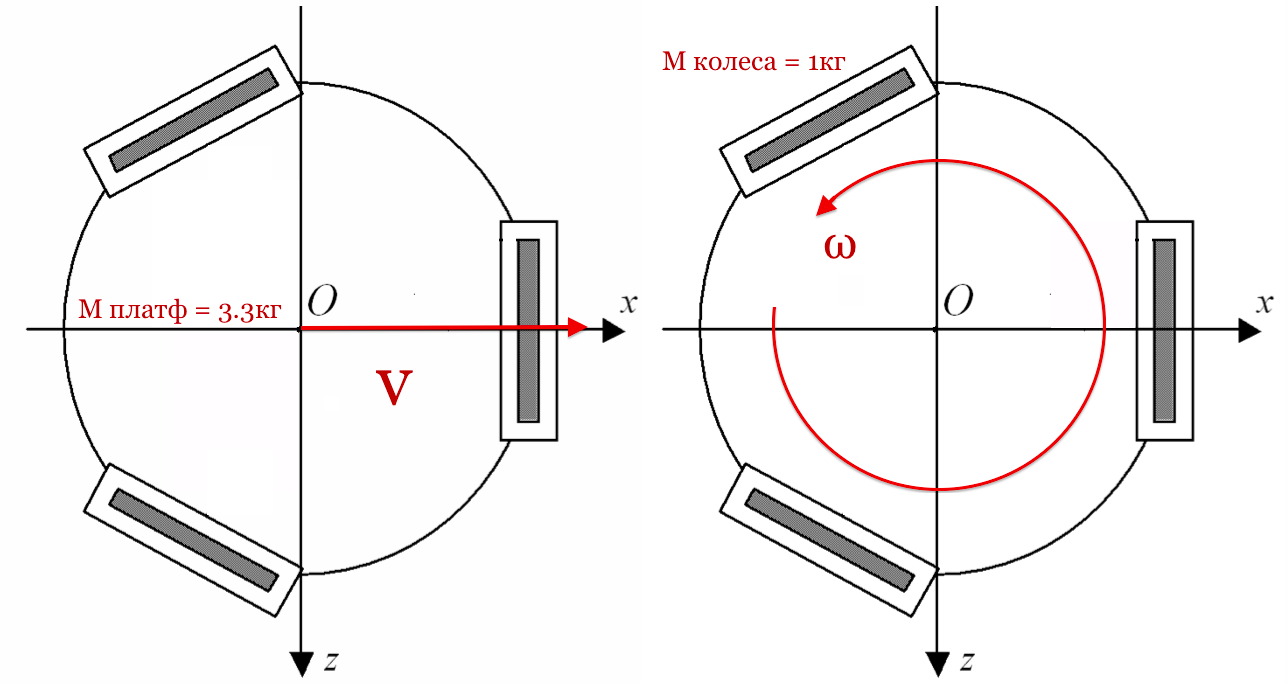
\includegraphics[width=0.95\textwidth]{content/parts/3_friction/diploma/img/art/my_exp_setup.png}
    \caption{Параметры экспериментов}
    \label{fig:my_exp_setup}
\end{figure}

При выполнении численных экспериментов массы платформы и колес, количество колес, количество роликов, геометрия системы были фиксированы (см. рис.~\ref{fig:my_exp_setup}). Изменялись начальные данные и доля массы роликов.\\

Испытания проводились, в частности, и для случая, когда относительная суммарная масса роликов приближается к нулю. В этом случае оказалось, что движение экипажа и омни-колес неограниченно приближаются к соответствующим функциям решения задачи Коши, получаемым в силу дифференциальных уравнений движения, используемых в работе~\cite{Borisov2011}, в которых динамика роликов не учитывается.

Рассмотрены два типа начальных условий $\vec{v}(0) = (v_0, 0, 0)^T, \omega(0) = \omega_0$ (см. рис.~\ref{fig:my_exp_setup}):
\begin{enumerate}
\item экипаж имеет начальную линейную скорость в направлении одного из колес и не закручен (ожидаемый результат - центр масс экипажа движется вдоль оси $Ox$, экипаж не вращается),
\item экипаж закручен вокруг вертикальной оси, проходящей через его центр масс, скорость центра масс равна нулю (ожидаемый результат - экипаж вращается вокруг своей вертикальной оси симметрии, и центр масс покоится).
\end{enumerate}

Значения отношения $\eta$ массы ролика к общей массе колеса принимали в обоих случаях значения от $10^{-6}n^{-1}$ до $10^{-1}n^{-1}$ с шагом $1$ по порядку малости (здесь $n$ - фиксированное количество роликов).

На рис.~\ref{fig:exp_examples} приведены примеры траектории центра масс $y(x)$ и зависимости $\psi(t)$ угла поворота $\psi$ платформы вокруг вертикальной оси, проходящей через её центр, для случаев 1) и 2). Кривые $y(x)$, изображающие траектории центра масс, соответствуют, в сущности, точке - началу координат - в случае $v_0 = 0, \omega_0 = 1$, и отрезку прямой, совпадающей с осью $x$, в случае $v_0 = 1, \omega_0 = 0$, ибо масштаб отображения таков, чтобы были видны отклонения от точных значений, возникающие в силу вычислительной погрешности, но сами эти отклонения имеют порядок малости, позволяющий считать их нулевыми. Аналогичное утверждение верно и для зависимости угла поворота платформы $\psi$ от времени в случае поступательного движения - полученная зависимость близка к постоянной.\\

Ниже представлены результаты нескольких численных экспериментов. Во всех случаях величины, изображенные на рис.~\ref{fig:exp_examples}, демонстрируют поведение, не различимое в масштабе рис.~\ref{fig:exp_examples}, и поэтому приведены лишь расхождения между построенной нами моделью и верификационной идеализацией, которые и представляют интерес. Также представлена абсолютная величина скорости скольжения в точке контакта в физической модели.\\

Графики зависимости скорости скольжения от времени показывают, что скольжение имеет место в окрестности момента смены роликов. Это объясняется тем, что для идеального качения в эти моменты ролику необходима бесконечная угловая скорость собственного вращения, ибо его размер вблизи вершины стремится к нулю. Видно, что с ростом доли массы роликов в общей массе колеса скольжение в контакте становится существеннее, изменяясь от пренебрежимо малого при $\eta = 10^{-6}$ до весьма существенного уже при $\eta = 10^{-3}$. Тем не менее, расхождения траектории и угла поворота платформы малы, а скольжение наблюдается лишь в точках колеса, которые в промышленных конструкциях не присутствуют (см. Обзор), что и позволяет считать верификацию проведенной.
\newpage

% EXAMPLES
\begin{figure}[h]
\centering
\begin{subfigure}{.47\textwidth}
    \centering
    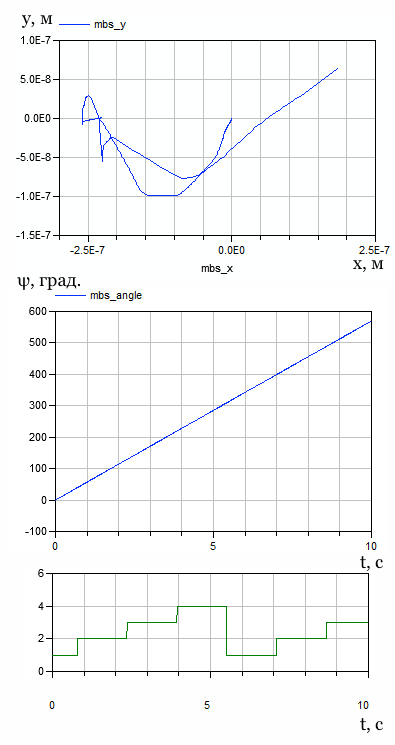
\includegraphics[width=\textwidth]{content/parts/3_friction/diploma/img/res/example_v_0_0_omega_1_frac_1e-1_n_4_time_10s.png}
    \caption{$\eta = 0,1, v_0 = 0, \omega_0 = 1$}
    \label{fig:exp_example_omega}
\end{subfigure}%
\hspace{5pt}
\begin{subfigure}{.47\textwidth}
    \centering
    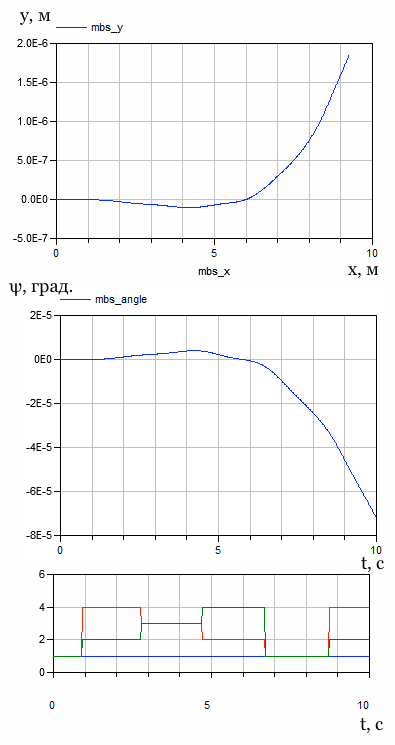
\includegraphics[width=\textwidth]{content/parts/3_friction/diploma/img/res/example_v_1_0_omega_0_frac_1e-1_n_4_time_10s.png}
    \caption{$\eta = 0,1, v_0 = 1, \omega_0 = 0$}
    \label{fig:exp_example_v}
\end{subfigure}
\caption{Примеры траекторий, характера изменения угла и смены номеров роликов в контакте для двух типов начальных условий. На нижнем графике - номер ролика в контакте, см. рис.~\ref{OmniWheel}}
\label{fig:exp_examples}
\end{figure}
\newpage

\begin{figure}[h]
\begin{center}\begin{equation*}\begin{array}{cc}
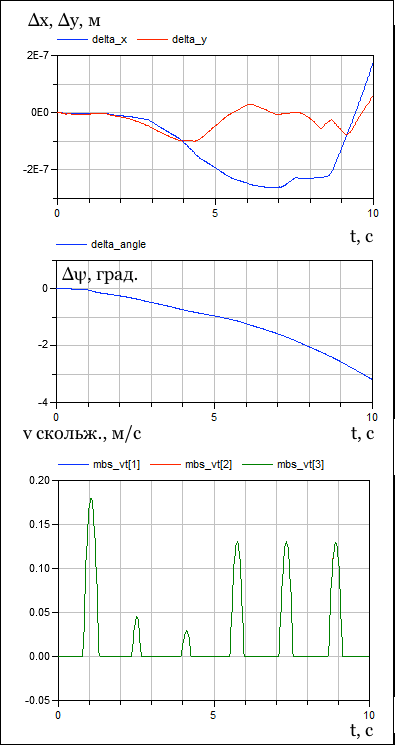
\includegraphics[width=7cm, viewport=0 0 395 745,clip]{content/parts/3_friction/diploma/img/res/comparison_v_0_0_omega_1_frac_1e-1_n_4_time_10s.png} & \includegraphics[width=7cm, viewport=0 0 395 745,clip]{content/parts/3_friction/diploma/img/res/comparison_v_0_0_omega_1_frac_1e-2_n_4_time_10s.png}\\
\eta = 0,1, v_0 = 0, \omega_0 = 1 & \eta = 0,01, v_0 = 0, \omega_0 = 1\\
\end{array}\end{equation*}\end{center}
\caption{Вращение экипажа с трением вокруг вертикальной оси}
\end{figure}
\newpage

\begin{figure}[h]
\begin{center}\begin{equation*}\begin{array}{cc}
\includegraphics[width=7cm, viewport=0 0 395 745,clip]{content/parts/3_friction/diploma/img/res/comparison_v_0_0_omega_1_frac_1e-3_n_4_time_10s.png} & \includegraphics[width=7cm, viewport=0 0 395 745,clip]{content/parts/3_friction/diploma/img/res/comparison_v_0_0_omega_1_frac_1e-4_n_4_time_10s.png}\\
\eta = 0,001, v_0 = 0, \omega_0 = 1 & \eta = 0,0001, v_0 = 0, \omega_0 = 1\\
\end{array}\end{equation*}\end{center}
\caption{Вращение экипажа с трением вокруг вертикальной оси}
\end{figure}
\newpage

\begin{figure}[h]
\begin{center}\begin{equation*}\begin{array}{cc}
\includegraphics[width=7cm, viewport=0 0 395 745,clip]{content/parts/3_friction/diploma/img/res/comparison_v_0_0_omega_1_frac_1e-5_n_4_time_10s.png} & \includegraphics[width=7cm, viewport=0 0 395 745,clip]{content/parts/3_friction/diploma/img/res/comparison_v_0_0_omega_1_frac_1e-6_n_4_time_10s.png}\\
\eta = 10^{-5}, v_0 = 0, \omega_0 = 1 & \eta = 10^{-6}, v_0 = 0, \omega_0 = 1\\
\end{array}\end{equation*}\end{center}
\caption{Вращение экипажа с трением вокруг вертикальной оси}
\end{figure}
\newpage

\begin{figure}[h]
\begin{center}\begin{equation*}\begin{array}{cc}
\includegraphics[width=7cm, viewport=0 0 395 745,clip]{content/parts/3_friction/diploma/img/res/comparison_v_1_0_omega_0_frac_1e-1_n_4_time_10s.png} & \includegraphics[width=7cm, viewport=0 0 395 745,clip]{content/parts/3_friction/diploma/img/res/comparison_v_1_0_omega_0_frac_1e-2_n_4_time_10s.png}\\
\eta = 0,1, v_0 = 1, \omega_0 = 0 & \eta = 0,01, v_0 = 1, \omega_0 = 0\\
\end{array}\end{equation*}\end{center}
\caption{Вращение экипажа с трением по прямой}
\end{figure}
\newpage

\begin{figure}[h]
\begin{center}\begin{equation*}\begin{array}{cc}
\includegraphics[width=7cm, viewport=0 0 395 745,clip]{content/parts/3_friction/diploma/img/res/comparison_v_1_0_omega_0_frac_1e-3_n_4_time_10s.png} & \includegraphics[width=7cm, viewport=0 0 395 745,clip]{content/parts/3_friction/diploma/img/res/comparison_v_1_0_omega_0_frac_1e-4_n_4_time_10s.png}\\
\eta = 0,001, v_0 = 1, \omega_0 = 0 & \eta = 0,0001, v_0 = 1, \omega_0 = 0\\
\end{array}\end{equation*}\end{center}
\caption{Вращение экипажа с трением по прямой}
\end{figure}
\newpage


\newpage
\bibliographystyle{./util/BibTeX-Styles/utf8gost705u}  %% стилевой файл для оформления по ГОСТу
\bibliography{content/library}   % name your BibTeX data base

\end{document}